\documentclass[a4paper, twoside, leqno, 11pt]{article}
\usepackage{preamble}

\begin{document}

\title{\bfseries\scshape\course}
\date{Весна 2025\,г.}
\author{Пшеничный Никита\thanks{Последняя компилляция: \today\ Актуальную версию этого файла можно найти на \href{https://github.com/pshenikita/Differential-Geometry}{моём GitHub}.}}

\maketitle
\begin{abstract}
	В основу этих записок легли лекции О.\,И. Мохова и семинары А.\,А. Гайфуллина на мехмате МГУ, а также (в меньшей степени) курс А.\,В. Пенского в НМУ.

	При написании файла я во многом ориентировался на \href{https://teach-in.ru/course/classical-difgeom-dynnikov}{лекции И.\,А. Дынникова по дифференциальной геометрии} и на начальные главы книги \cite{NT14} (в особенности на главу 3). Некоторые из разобранных задач взяты из классического <<Сборника задач по дифференциальной геометрии>> А.\,С. Мищенко, Ю.\,П. Соловьёва, А.\,Т. Фоменко (далее именуемого просто <<задачником>>).

	В конце каждого раздела приведены пояснения к появляющимся в тексте эпиграфам. Конечно, эти эпиграфы носят в основном юмористический (или ностальгический\ldots) характер, но у большинства из них есть содержательный математический контекст.

	\begin{thebibliography}{9}
	\bibitem[Новиков "---Тайманов]{NT14} С.\,П. Новиков, И.\,А. Тайманов, \textit{Современные геометрические структуры и поля}. МЦНМО, 2014.
	\bibitem[Шарп]{S19} Ричард У.\,Шарп, \textit{Дифференциальная геометрия. Обобщение Картана Эрлангенской программы Клейна}. МЦНМО, 2019.
\end{thebibliography}


\end{abstract}

\tableofcontents

\subsection*{Обозначения}

\begin{center}
\begin{minipage}{.9\textwidth}
	$\R$ --- поле (топологическое пространство) вещественных чисел;

	$\vec{x} = (x^1, \ldots, x^n)$ --- вектор (точка) из $\R^n$;
	
	$(\vec{e}_1, \ldots, \vec{e}_n)$ --- стандартный базис в $\R^n$;

	$\span(\vec{v}_1, \ldots, \vec{v}_n)$ --- линейная оболочка векторов $\vec{v}_1, \ldots, \vec{v}_n$;

	$S_{\Or}(\vec{u}, \vec{v})$ --- ориентированная площадь параллелограмма, натянутого на векторы $\vec{u}$ и $\vec{v}$, $\Vol_{\Or}(\vec{v}_1, \ldots, \vec{v}_n)$ --- ориентированный объём $n$-мерного параллелепипеда, натянутого на векторы $\vec{v}_1,\,\ldots,\,\vec{v}_n$;

	$I$ --- связное подмножество $\R$;

	$\Int U$ --- внутренность подмножества $U \subset \R^n$;

	$\langle\vec{x}, \vec{y}\rangle$ --- евклидово скалярное произведение векторов $\vec{x},\,\vec{y} \in \R^n$;

	$\langle\vec{x}, \vec{y}\rangle_\G$ --- скалярное произведение векторов $\vec{x},\,\vec{y} \in \R^n$, задаваемое положительно определённой симметричной матрицей $\G$ (то есть $\langle\vec{x}, \vec{y}\rangle_\G = \vec{x}^t\G\vec{y}$);

	$\vec{x} \times \vec{y}$ --- векторное произведение векторов $\vec{x},\,\vec{y} \in \R^3$;

	$\rho(\vec{x}, \vec{y})$ --- расстояние между точками $\vec{x}$ и $\vec{y}$ из $\R^n$;

	$\vec{r}(t) = (x^1(t), \ldots, x^n(t))$ --- радиус-вектор точки $\vec{x} \in \R^n$;

	$\dot{\vec{r}}(t),\,\ddot{\vec{r}}(t),\,\ldots$ --- векторы скорости, ускорения и т.\,д. точки $\vec{x} \in \R^n$.

	\medskip
	\textbf{Нотация Эйнштейна}. {\small По дважды повторяющимся индексам, один из которых верхний, а другой нижний, подразумевается суммирование в пределах, устанавливаемых из контекста, а сам такой индекс называется \textit{слепым}. Верхний индекс переменной, появляющейся в знаменателе, считается для выражения нижним, и наоборот.}
\end{minipage}
\end{center}

\section{Предварительные сведения и напоминания}

\epigraph{Сначала вы подумаете, что я сумасшедший, а потом вам понравится, и вы сами будете делать так же.}{А.\,В. Пенской}

\subsection{Математический анализ}

Отображение $\vec{f}\colon \R^n \to \R^m$ называется \textit{дифференцируемым в точке} $\vec{x}_0$, если существует линейное отображение $\mathcal{L}_{\vec{x}_0}$, для которого выполнено
\[
	\vec{f}(\vec{x}) = \vec{f}(\vec{x}_0) + \mathcal{L}_{\vec{x}_0}(\vec{x} - \vec{x}_0) + \o(\norm{\vec{x} - \vec{x}_0})\text{ при $\vec{x} \to \vec{x}_0$}.
\]

При этом отображение $\vec{f}$ не обязано быть определено всюду. Нам будет достаточно, чтобы в область определения отображения $\vec{f}$ входило замыкание некоторой выпуклой открытой области, содержащее точку $\vec{x}_0$. Однозначно определённое линейное отображение $\mathcal{L}_{\vec{x}_0} = \vcentcolon \left.d\vec{f}\right|_{\vec{x_0}}$ называют \textit{дифференциалом} отображения $\vec{f}$ в точке $\vec{x}$.

Матрица $J_{\vec{f}}(\vec{x}_0)$ линейного отображения $\left.d\vec{f}\right|_{\vec{x}_0}$ называется \textit{матрицей Якоби} отображения $\vec{f}$ в точке $\vec{x}_0$ и состоит из \textit{частных производных}:

\[
	J_{\vec{f}}(\vec{x}_0) =
	\begin{pmatrix}
		\ds\left.\frac{\partial f^1}{\partial x^1}\right|_{\vec{x}_0} & \ds\ldots & \ds\left.\frac{\partial f^1}{\partial x^n}\right|_{\vec{x}_0} \\
		\ds\vdots & \ds\ddots & \ds\vdots \\
		\ds\left.\frac{\partial f^m}{\partial x^1}\right|_{\vec{x}_0} & \ds\ldots & \ds\left.\frac{\partial f^m}{\partial x^n}\right|_{\vec{x}_0} \\
	\end{pmatrix} =
	\begin{pmatrix}
		\left.\nabla f^1\right|_{\vec{x}_0} \\
		\vdots\\
		\left.\nabla f^m\right|_{\vec{x}_0} \\
	\end{pmatrix}.
\]
В случае, когда эта матрица квадратная, её определитель называют \textit{якобиантом}.

Дифференцируемое отображение $\vec{f}$ определяет новое отображение $\partial \vec{f} / \partial \vec{x}\colon \R^n \to \R^m$. Если последнее также дифференцируемо, то $\vec{f}$ называется \textit{дважды дифференцируемым}, и далее индуктивно: если $\partial\vec{f} / \partial\vec{x}$ дифференцируемо $k$ раз, то $\vec{f}$ дифференцируемо $k + 1$ раз. Если отображение $\vec{f}$ дифференцируемо $k$ раз и при $k$-кратном дифференцировании получается непрерывное отображение, то говорят, что $\vec{f}$ \textit{$k$ раз непрерывно дифференцируемо} или является \textit{отображением класса $C^k$}. В дальнейшем под \textit{гладким отображением} мы будем подразумевать отображение класса $C^k$ для достаточно большого $k$.

\begin{theorem}[О производной сложной функции]
	Если отображения $\vec{f}\colon \R^n \to \R^m$ и $\vec{g}\colon \R^m \to \R^k$ дифференцируемы, то дифференцируема и композиция $\vec{g} \circ \vec{f}$, причём
	\[
		\left.d(\vec{g} \circ \vec{f})\right|_{\vec{x}_0} = \left.d\vec{g}\right|_{\vec{f}(\vec{x_0})} \circ \left.d\vec{f}\right|_{\vec{x}_0}.
	\]
\end{theorem}

\begin{theorem}[Об обратном отображении]
	Гладкое отображение $\vec{f}\colon \R^n \to \R^n$, матрица Якоби которого невырожденна в точке $\vec{x}_0$, локально обратимо в некоторой окрестности точки $\vec{x}_0$, причём обратное отображение также гладкое.
\end{theorem}

\begin{theorem}[О неявном отображении]
	Пусть $\vec{f}\colon \R^n \to \R^m$, $m \leqslant n$, --- гладкое отображение, матрица Якоби которого в точке $\vec{x}_0$ имеет ранг $m$. Тогда множество решений уравнения $\vec{f}(\vec{x}) = \vec{f}(\vec{x}_0)$ в окрестности точки $\vec{x}_0$ выглядит как график гладкого отображения, выражающего некоторые $m$ координат через оставшиеся $n - m$, причём эти $m$ координат можно выбрать те, которым соответствуют линейно независимые столбцы в матрице Якоби.
\end{theorem}

\subsection{Аналитическая геометрия и линейная алгебра}

Пусть в $\R^n$ есть некоторая поверхность, задаваемая уравнением $F(x^1, \ldots, x^n) = 0$, а по ней движется точка, радиус-вектор которой есть $\vec{x} = \vec{r}(t)$. Тогда можем продифференцировать тождество $F(r^1(t), \ldots, r^n(t)) = 0$ в каждой точке, получив по теореме о сложной функции
\[
	\frac{\partial F}{\partial r^1} \cdot \frac{d r^1}{dt} + \ldots + \frac{\partial F}{\partial r^n} \cdot \frac{d r^n}{dt} = 0
\]
или, что то же, $\langle \nabla F, \dot{\vec{r}} \rangle = 0$.

Из правила Лейбинца сразу следует формула дифференцирования скалярного произведения:
\[
	\frac{d}{dt}\langle \vec{a}(t), \vec{b}(t) \rangle = \langle \dot{\vec{a}}(t), \vec{b}(t) \rangle + \langle \vec{a}(t), \dot{\vec{b}}(t) \rangle.
\]

Важный частный случай: если $\vec{a}(t) \perp \vec{b}(t)$ для всех значений параметра $t$, то $\langle\vec{a}(t), \dot{\vec{b}}(t)\rangle \hm= -\langle\dot{\vec{a}}(t), \vec{b}(t)\rangle$. Аналогичная формула верна и для векторного произведения:
\[
	\frac{d}{dt}(\vec{a}(t) \times \vec{b}(t)) = (\dot{\vec{a}}(t) \times \vec{b}(t)) + (\vec{a}(t) \times \dot{\vec{b}}(t)).
\]

Пусть $\vec{r}\colon \R \to \R^n$. Тогда $\abs{\vec{r}} = \const$ тогда и только тогда, когда $\langle \vec{r}, \dot{\vec{r}} \rangle = 0$. Доказательство простое --- надо продифференцировать тождество $\langle \vec{r}(t), \vec{r}(t) \rangle = \const$. Можно доказать и по-другому --- вектор постоянной длины $\abs{\vec{r}} = \const$ лежит на сфере, уравнение которой $F(x_1, \ldots, x_n) = x_1^2 + \ldots + x_n^2 = \const$. При этом
\[\begin{tikzcd}
	{0} & {\langle\nabla{F}, \dot{\vec{r}}\rangle} & {\langle 2\vec{r}, \dot{\vec{r}}\rangle = 2\langle\vec{r}, \dot{\vec{r}}\rangle}.
	\arrow[equals, from=1-2, to=1-1]
	\arrow[equals, from=1-2, to=1-3]
\end{tikzcd}\]

Проекция вектора $\vec{u}$ на вектор $\vec{v}$ вычисляется по формуле
\[
	\proj_{\vec{v}}\vec{u} = \frac{\langle\vec{u}, \vec{v}\rangle}{\langle\vec{v}, \vec{v}\rangle} \cdot \vec{v}.
\]

Объём сведений из линейной алгебры, которые необходимы в курсе дифференциальной геометрии (и в других дисциплинах), начинается становиться слишком большим для маленького раздела напоминаний в этом файле, поэтому я решил вынести его в отдельный проект, которым скоро начну заниматься (здесь появится ссылка на него).

\subsection{Про функции в геометрии}

Фразу, упомянутую в эпиграфе к данному разделу, А.\,В. Пенской произнёс на первой лекции своего курса по дифференциальной геометрии в 2025\,г.

Рассмотрим евклидову плоскость\footnotemark{} $\mathbb{E}^2$ и фиксированную точку $O$ на ней. Пусть на этой плоскости задана функция $f(\vec{x}) = \big|\overrightarrow{O\vec{x}}\big|$ (измеряем евклидово расстояние до заданной точки). Мы можем ввести евклидовы координаты в этой плоскости, в них наша функция записывается как $f(x, y) = \sqrt{x^2 + y^2}$. А можем ввести полярные, и тогда функция записывается как $f(\rho, \varphi) = \rho$. Наблюдаем некоторое противоречие --- одна и та же функция $f$ от двух аргументов записывается двумя (очевидно, различными) способами, то есть формально нельзя написать $f(x, y) = f(\rho, \varphi)$. Но мы так пишем, и мы на самом деле хотим так писать. Так в чём же дело?

\footnotetext{Везде в тексте, кроме этого комментария, евклидово пространство размерности $n$ отождествляется с $\R^n$. Здесь важно сохранить обозначения Алексея Викторовича.} 

Корень этого мнимого противоречия заключается в том, как мы думаем о функциях в алгебре и анализе. Мы привыкли к тому, что функция --- это <<алгоритм вычисления>>. С этой точки зрения $f(\rho, \varphi)$ должно быть равно $\sqrt{\rho^2 + \varphi^2}$, но ведь ясно, что мы имеем в виду не это. А на самом деле происходит следующее.

\shorthandoff{"}%
\[\begin{tikzcd}
	{\underset{\mathclap{x,\,y}}{\mathbb{R}}^2} \\
	& {\mathbb{E}^2} && {\mathbb{R}} \\
	{\underset{\mathclap{\rho,\,\varphi}}{\mathbb{R}}^2}
	\arrow["\Phi", from=1-1, to=2-2]
	\arrow["f", from=2-2, to=2-4]
	\arrow["\Psi"', from=3-1, to=2-2]
\end{tikzcd}\]
\shorthandon{"}%

Имеет место такая коммутативная диаграмма, где отображения $\Phi$ и $\Psi$ задают выбор системы координат. Запись $f(x, y) = \sqrt{x^2 + y^2}$ формально некорректна, ведь на самом деле таким образом задаётся не функция $f$, а композиция $(f \circ \Phi)(x, y) = \sqrt{x^2 + y^2}$. Так же можно написать и в полярных координатах: $(f \circ \Psi)(\rho, \varphi) = \rho$. И то, что мы имеем в виду под записью $f(x, y) = f(\rho, \varphi)$, формально записывается как
\[
	f \circ \Phi = f \circ \Psi.
\]

Сама функция $f$ задана абстрактно, в её определении не фигурировали координаты, поэтому писать $f(x, y) = \ldots$ (или $f(\rho, \varphi) = \ldots$) формально нельзя. Но мы, конечно же, будем, потому что для нас первично абстрактное задание функции, а не система координат (или параметризация), в которой мы хотим её записать.

Теперь можем написать ещё более <<удивительную>> формулу:
\[
	f(\rho, \varphi) = f\big(x(\rho, \varphi),\,y(\rho, \varphi)\big).
\]

Если уж мы согласились с равенством $f(\rho, \varphi) = f(x, y)$, то мы обязаны согласиться и с этим равенством, ведь от первого ко второму можно перейти, рассматривая $x$ и $y$ как функции $x(\rho, \varphi) = \rho\cos\varphi$, $y(\rho, \varphi) = \rho\sin\varphi$. И мы действительно можем с ним согласиться, ведь формально это равенство можно записать как
\[
	f \circ \Psi = (f \circ \Phi) \circ (\Phi^{-1} \circ \Psi).
\]


\section{Теория кривых}

\epigraph{Рубины шлифуют алмазами.}{А.\,А. Гайфуллин}

\subsection{Базовые определения}

\begin{definition}
	\textit{Простой дугой} $\gamma$ в $\R^n$ называется любое подмножество $\R^n$, гомеоморфное отрезку $[0; 1]$. \textit{Параметризацией} простой дуги называется гомеоморфизм $\vec{r}\colon [0; 1] \to \gamma$.
\end{definition}

\begin{definition}
	Параметризация $\vec{r}\colon [0; 1] \to \R^n$ простой дуги называется \textit{регулярной класса $C^k$}, если для всех $i = 1, \ldots, n$ функция $r^i(t)$ является отображением класса $C^k$ и
	\[
		\frac{d\vec{r}}{dt} \ne \vec{0}
	\]
	в каждой точке (для концов отрезка $0$ и $1$ в качестве производной берётся производная справа и слева соответственно). Простая дуга называется \textit{регулярной}, если существует её регулярная параметризация.
\end{definition}

%Параметризация простой дуги естественным образом задаёт на ней ориентацию, и в дальнейшем нам будет удобно, чтобы при сменах параметра эта ориентация сохранялась. Иными словами, мы будем рассматривать только такие замены параметра $s = \varphi(t)$, для которых $d\varphi / dt > 0$. При этом векторы $\frac{d\vec{r}}{ds}$ и $\frac{d\vec{r}}{dt} = \frac{d\vec{r}}{ds}\frac{ds}{dt}$ всюду остаются сонаправленными.

\begin{definition}
	\textit{Параметризованной кривой} в $\R^n$ называется непрерывное отображение $\vec{r}\colon I \to \R$ такое, что существует не более чем счётное покрытие промежутка $I$ отрезками $[a_i; b_i]$ такое, что для каждого $i$ ограничение $\left.\vec{r}\right|_{[a_i; b_i]}$ есть параметризация простой дуги.
\end{definition}

\begin{definition}
	\textit{Кривой} в $\R^n$ называется класс эквивалентности параметризованных кривых, где $\vec{r}_1\colon I_1 \to \R^n$ и $\vec{r}_2\colon I_2 \to \R^n$ \textit{эквивалентны}, если существует такой гомеоморфизм $I_1 \to I_2$, что следующая диаграмма коммутативна:
	\shorthandoff{"}%
	\begin{equation*}
		\begin{tikzcd}
			I_1 && {\R^n} \\
			\\
			I_2 && {\R^n}
			\arrow["\vec{r}_1", hook, from=1-1, to=1-3]
			\arrow["\cong"', from=1-1, to=3-1]
			\arrow["\id", from=1-3, to=3-3]
			\arrow["\vec{r}_2", hook, from=3-1, to=3-3]
		\end{tikzcd}
	\end{equation*}
	\shorthandon{"}%
	Любое вложение из данного класса будем называть \textit{параметризацией} кривой.
\end{definition}

\begin{definition}
	Кривая в $\R^n$ называется \textit{регулярной}, если она допускает \textit{регулярную параметризацию}, то есть гладкую параметризацию $\vec{r}\colon I \to \R^n$, для которой всюду $\dot{\vec{r}}(t) \ne \vec{0}$.
\end{definition}

В дальнейшем мы будем рассматривать только регулярные кривые. Условие регулярности необходимо добавить для соответствия интуитивному пониманию гладкости как отсутствия изломов.
\begin{figure}[h]
	\centering
	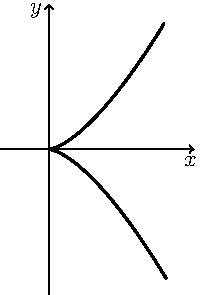
\includegraphics[height=5cm]{./img/SemicubicalParabola.pdf}
	\caption{Полукубическая парабола}
	\label{fig:SemicubicalParabola}
\end{figure}
Например, мы не хотим рассматривать кривые вроде $\vec{r}(t) = (t^2, t^3)$ (рис. \ref{fig:SemicubicalParabola}), хотя обе координатные функции $x(t) = t^2$ и $y(t) = t^3$ гладкие класса $C^\infty$.

\begin{proposition} \label{proposition:SmoothHomeomorphism}
	Если $\vec{r}_1(t)$ и $\vec{r}_2(s)$ --- регулярные эквивалентные параметризации, то $t(s)$ и $s(t)$ являются гладкими функциями.
\end{proposition}

\begin{proof}
	Рассмотрим параметр $t$. Так как обе параметризации регулярны, то $\dot{\vec{r}}_1(t_0) \ne 0$ в каждой точке $t_0$. Тогда найдётся номер $i_0$ такой, что $\dot{x}^{i_0}(t_0) \ne 0$. Тогда по теореме об обратной функции в некоторой окрестности точки $t_0$ можно выразить параметр $t$ через $x^{i_0}$, то есть $t(x^{i_0})$ --- гладкая функция в некоторой окрестности данной точки. А $x^{i_0}$, в свою очередь, является гладкой функцией от $s$ (так как отображение $\vec{r}_2$ гладкое). Таким образом, функция $t(s) = t(x^{i_0}(s))$ гладкая как композиция гладких функций (теорема о сложной функции). Аналогично доказывается, что функция $s(t)$ тоже гладкая.
\end{proof}

Важно подчеркнуть, что при доказательстве использовалось рассуждение, которое можно сформулировать так: на регулярной кривой в некоторой окрестности любой точки можно в качестве регулярного параметра выбрать одну из координат евклидова пространства. Отсюда легко сразу получить нерегулярность полукубической параболы (рис. \ref{fig:SemicubicalParabola}) --- легко видеть, что в окрестности точки $(0, 0)$ её нельзя регулярно параметризовать ни одной переменной $x$ или $y$.

Регулярная параметризация кривой естественным образом определяет на ней ориентацию как направление возрастания параметра. Дадим более точное определение.

\begin{definition}
	\textit{Ориентацией} регулярной кривой называется класс эквивалентности её параметризаций с положительным якобианом перехода.
\end{definition}

То есть, регулярные параметры $t$ и $s$ задают одинаковую ориентацию кривой, если и только если всюду выполнено $ds / dt > 0$. Легко видеть, что ориентаций на кривой ровно две.

\subsection{Способы задания кривой}

На практике часто приходится иметь дело с кривыми, заданными с помощью уравнений. С глобальной точки зрения данный подход не эквивалентнен параметрическому заданию. Однако, если наложить на систему уравнений некоторые ограничения, то мы получим объекты, локально устроенные так же, как кривые.

\begin{definition}
	Пусть $\vec{f}$ --- гладкая функция из некоторого подмножества $U \subset \R^n$ в $\R^m$, $m \leqslant n$. Мы говорим, что точка $\vec{x}_0 \in U$ является для неё \textit{регулярной}, если $\vec{x}_0 \in \Int U$ и $\rk J_{\vec{f}}(\vec{x}_0) = m$.
\end{definition}

\begin{theorem} \label{theorem:SurfacesToCurve}
	Пусть $f_1, \ldots, f_{n - 1}$ --- набор гладких функций из некоторого подмножества $U \subset \R^n$ в $\R$, а точка $\vec{x}_0 \in U$ является регулярной точкой отображения $\vec{f} = (f_1, \ldots, f_{n - 1})$ и решением системы уравнений
	\[
		\begin{cases}
			f_1(\vec{x}) = 0,\\
			\dotfill\\
			f_{n - 1}(\vec{x}) = 0,
		\end{cases}
	\]
	то есть $\vec{f}(\vec{x}_0) = \vec{0}$. Тогда существует окрестность точки $\vec{x}_0$, в которой пространство решений этой системы представляет собой гладкую регулярную кривую.
	
	Верно и обратное: в окрестности любой точки регулярной кривой её можно задать системой уравнений, которая регулярна в этой точке.
\end{theorem}

\begin{proof}
	Без ограничения общности, можем считать, что первые $n - 1$ столбцов матрицы $J_{\vec{f}}(\vec{x}_0)$ линейно независимы (иначе перенумеруем координаты). Тогда по теореме о неявной функции решение этой системы в некоторой окрестности точки $\vec{x}_0$ задаётся гладкими функциями $x^1(x^n), \ldots, x^{n - 1}(x^n)$. Но это и означает, что локально решения представляют собой регулярную кривую, так как радиус-вектор параметризован последней координатой: $\vec{r}(x^n) = (x^1(x^n), \ldots, x^{n - 1}(x^n), x^n)$. Эта параметризация регулярна, поскольку последней компонентой вектора скорости $\dot{\vec{r}}$ будет $1$.

	Докажем обратное утверждение. Как упоминалось в предложении \ref{proposition:SmoothHomeomorphism}, в качестве параметра локально можно взять одну из координат. Не теряя общности, будем считать, что эта координата $x^n$: $\vec{r}(x^n) = (x^1(x^n), \ldots, x^{n - 1}(x^n), x^n)$. Теперь запишем систему уравнений $\vec{x} - \vec{r}(x^n) = \vec{0}$, которая локально задаёт нашу кривую. Первые $n - 1$ столбец матрицы Якоби $J_{\vec{x} - \vec{r}(x^n)}$ в рассматриваемой точке составляют единичную матрицу.
\end{proof}

\subsection{Касательная в точке регулярной кривой}

\begin{definition}
	Пусть регулярная кривая задана радиус-вектором $\vec{r}(t)$. \textit{Касательная прямая} к этой кривой в точке $t_0$ задаётся рядом Тейлора функции $\vec{r}$ с отбрасыванием всех членов более высокого порядка, чем $t - t_0$:
	\[
		\vec{\ell}(t) \vcentcolon = \vec{r}(t_0) + \left.\frac{d\vec{r}}{dt}\right|_{t_0}(t - t_0).
	\]
\end{definition}

Нужно проверить корректность данного определения, ведь оно сформулировано для конкретной параметризации кривой. Здесь корректность сразу следует из предложения \ref{proposition:SmoothHomeomorphism} и теоремы о сложной функции:
\[
	\frac{d\vec{r}}{dt} = \frac{d\vec{r}}{ds} \frac{ds}{dt}.
\]

\begin{theorem}
	\begin{enumerate}[nolistsep, label=(\arabic*)]
		\item Пусть $\gamma$ --- регулярная кривая, $\vec{x}_0 \in \gamma$ --- некоторая её точка, $\ell$ --- касательная прямая в точке $\vec{x}$. Тогда для $\vec{x}_1 \in \gamma$, $\vec{x}_1 \ne \vec{x}_0$ выполнено
			\[
				\rho(\vec{x}_1, \ell) = \o(\abs{\vec{x}_1 - \vec{x}_0})\text{ при $\vec{x}_1 \to \vec{x}_0$}.
			\]
		\item Для каждой точки $\vec{x}_0 \in \gamma$ касательная прямая является единственной прямой с указанным свойством.
	\end{enumerate}
\end{theorem}

\begin{proof}
	Пусть на $\gamma$ выбрана регулярная параметризация $\vec{r}(t)$, в которой $\vec{x}_0 \hm= \vec{r}(0)$. В качестве точки $\vec{x}_1$ будем брать $\vec{r}(t)$, где $t$ пробегает окрестность нуля. Условие $\vec{r}(t) \to \vec{x}_0$ можно заменить на $t \to 0$ (по определению кривой). Обозначим $\vec{v}_0 \vcentcolon = \dot{\vec{r}}(0)$. По условию, $\vec{v}_0 \ne 0$.
	\begin{enumerate}[nolistsep, label=(\arabic*)]
		\item По формуле Тейлора имеем
			\[
				\vec{r}(t) = \vec{x}_0 + \vec{v}_0t + \o(t) = \vec{x}_0 + (\vec{v}_0 + \o(1))t\text{ при $t \to 0$}.
			\]
			Расстояние от $\vec{r}(t)$ до прямой $\ell$ равно $\rho(\vec{r}(t), \ell) = \abs{\vec{r}(t) - \vec{x}_0}\sin\alpha(t)$, где $\alpha(t)$ --- угол между векторами $\vec{v}_0$ и $\vec{r}(t) - \vec{x}_0$. Поскольку $\vec{r}(t) - \vec{x}_0 = (\vec{v}_0 + \o(1))t$, этот угол равен $\o(1)$ при $t \to 0$. Получаем
			\[
				\rho(\vec{r}(t), \ell) = \abs{\vec{r}(t) - \vec{x}_0}\o(1) = \o(\abs{\vec{r}(t) - \vec{x}_0}).
			\]
			\begin{figure}[H]
				\centering
				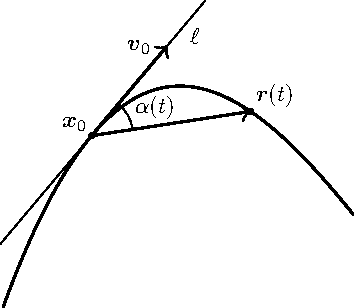
\includegraphics[width=6cm]{./img/Curve.pdf}
				\caption[format=empty]{}
			\end{figure}
		\item Пусть теперь $\ell^\prime$ --- другая прямая, проходящая через точку $\vec{x}_0$, и пусть $\vec{u}$ --- её направляющий вектор. Тогда
			\[
				\rho(\vec{r}(t), \ell^\prime) = \abs{\vec{r}(t) - \vec{x}_0}\sin\beta(t),
			\]
			где $\beta(t)$ --- угол между векторами $\vec{u}$ и $\vec{r}(t) - \vec{x}_0 = (\vec{v}_0 + \o(1))t$. При $t \to 0$ угол $\beta(t)$ стремится к углу между векторами $\vec{u}$ и $\vec{v}_0$, который по предположению отличен от $0$ и $\pi$. Отсюда $\rho(\vec{r}(t), \ell^\prime) = \abs{\vec{r}(t) - \vec{x}_0}(\const + \o(1))$, где $\const \ne 0$.
	\end{enumerate}
\end{proof}

\begin{proposition}
	Если кривая в $\R^n$ задана системой уравнений $\vec{f}(\vec{x}) = \vec{0}$, то касательная к ней в регулярной точке $\vec{x}_0$ задаётся системой уравнений $J_{\vec{f}}(\vec{x}_0) \cdot (\vec{x} - \vec{x}_0) = 0$.
\end{proposition}

\begin{proof}
	Точка $\vec{x}_0$ регулярна для отображения $\vec{f}$, значит, $\rk J_{\vec{f}}(\vec{x}_0) = n - 1$, поэтому пространство решений системы с этой матрицей одномерно, то есть задаёт прямую в пространстве $\R^n$ (очевидно, проходящую через точку $\vec{x}_0$). Остаётся проверить, что эта прямая параллельна вектору скорости касательной прямой в точке $\vec{x}_0$.

	Пусть $\vec{r}(t)$ --- регулярная параметризация данной кривой в окрестности точки $\vec{x}_0 \hm= \vec{r}(t_0)$ (существует по теореме \ref{theorem:SurfacesToCurve}). Это означает, что $\vec{f}(\vec{r}(t)) = 0$ для всех $t$ из прообраза данной окрестности. По теореме о производной сложной функции имеет место равенство
	\[
		\frac{d}{dt}\vec{f}(\vec{r}(t)) = \left.\frac{\partial\vec{f}}{\partial\vec{x}}\right|_{\vec{r}(t)}\dot{\vec{r}}(t).
	\]
	Подставляя $t = t_0$, получаем
	\[
		\left.\frac{\partial\vec{f}}{\partial\vec{x}}\right|_{\vec{x}_0}\vec{v}_0 = 0,
	\]
	где $\vec{v}_0$ --- вектор скорости при $t = t_0$.
\end{proof}

\subsection{Натуральный параметр и кривизна}

\begin{definition}
	\textit{Длиной} кривой, заметаемой при изменении значения параметра от $t_0$ до $t$, называется число
	\[
		l = \int\limits_{t_0}^t\abs{\dot{\vec{r}}(t)}dt.
	\]
\end{definition}

Здесь опять нужно проверить корректность, то есть независимость от параметризации. Пусть мы перешли к другому регулярному параметру $s$ с сохранением ориентации. Тогда имеем
\[
	\int\limits_{s_0}^s\abs{\frac{d\vec{r}}{ds}}ds = \int\limits_{t_0}^t\abs{\frac{d\vec{r}}{dt}\frac{dt}{ds}}\frac{ds}{dt}dt = \int\limits_{t_0}^t\abs{\frac{d\vec{r}}{dt}}\frac{\cancel{dt}}{\cancel{ds}}\frac{\cancel{ds}}{\cancel{dt}}dt = \int\limits_{t_0}^t\abs{\frac{d\vec{r}}{dt}}dt.
\]

Мы намеренно допускаем отрицательную длину участка кривой (если $t_0 > t$), получая ориентированную длину кривой. И эта ориентация согласована с той, что мы обсуждали при определении параметризованной кривой. (Легко видеть, что при смене ориентации на кривой величина $l$ меняет знак.)

\begin{definition}
	Параметр $s$ называется \textit{натуральным параметром} регулярной кривой, если $\abs{d\vec{r} / ds} = 1$.
\end{definition}

\begin{proposition} \label{proposition:LengthParameter}
	\begin{enumerate}[nolistsep, label=(\arabic*)]
		\item Длина кривой $l(t)$ является натуральным параметром.
		\item Если $s$ --- некоторый натуральный параметр, то $s = \pm l + \const$.
	\end{enumerate}
\end{proposition}

\begin{proof}
	\begin{enumerate}[nolistsep, label=(\arabic*)]
		\item $dl / dt = \abs{d\vec{r} / dt} > 0$. Значит, по теореме об обратной функции можем локально выразить $t = t(l)$, и при этом
			\[
				\abs{\frac{d\vec{r}}{dl}} = \abs{\frac{d\vec{r}}{dt}\frac{dt}{dl}} = \frac{dt}{dl}\abs{\frac{d\vec{r}}{dt}} = \frac{\abs{d\vec{r} / dt}}{\abs{d\vec{r} / dt}} = 1.
			\]
		\item Если $s$ --- натуральный параметр, то $\abs{\dot{\vec{r}}(s)} = 1$ для каждого $s$. Отсюда,
			\[
				\pm l(s) = \int\limits_{s_0}^s\abs{\dot{\vec{r}}(s)}ds = s - s_0,
			\]
			то есть $s = \pm l + s_0$, что и требовалось. Знак <<$\pm$>> в начале последней формулы стоит для учёта ориентации параметра $s$, ведь она может быть не согласованной с выбором ориентации для длины кривой.
	\end{enumerate}
\end{proof}

Далее, если не указано иное, через $s$ мы будем всегда обозначать натуральный параметр, а через $\dot{\vec{r}}$ --- производную по натуральному параметру.

Предложение \ref{proposition:LengthParameter} говорит нам о том, что натуральный параметр на любой кривой можно выписать явно по формуле длины кривой. Наличие такой формулы говорит нам о том, что у кривых тривиальная внутренняя геометрия. Всё, что можно делать на кривой --- мерять длины, и мы (теоретически\footnotemark) можем это делать в любой параметризации.

\footnotetext{На практике интеграл в формуле длины кривой <<не берётся>>, если его специально не подобрали.}

При изучении кривых кажется естественным ввести величину, которая будет измерять, насколько сильно кривая отличается от прямой. Предлагается определить \textit{вектор кривизны} $\vec{k} \vcentcolon = \ddot{\vec{r}}$ (здесь на $\vec{r}$ введён натуральный параметр). Действительно, на прямых (и только на них) имеем $\vec{k} \equiv \vec{0}$, поэтому отличие этого вектора от нулевого может говорить нам о том, насколько кривая <<искривлена в пространстве>>.

\begin{definition}
	\textit{Кривизной} кривой в точке $s$ называется величина $k(s) \vcentcolon = \abs{\vec{k}(s)} = \abs{\ddot{\vec{r}}(s)}$. (Легко видеть, что кривизна не зависит от выбора натурального параметра $s$.)
\end{definition}

Это определение очень наглядное. Для простоты обсудим плоский случай. Можно представить, что мы едем по машине на ровной плоскости, вырисовывая колёсами гладкую регулярную кривую. Если мы будем ехать с единичной скоростью (то есть, на кривой будет выбран натуральный параметр), то в нашей плоскости на машину будет действовать только центробежная сила. Согласно второму закону Ньютона, эта сила равна произведению массы на ускорение. Нормировав массу автомобиля, получим векторное равенство силы и ускорения. Ранее кривизной кривой мы назвали длину вектора ускорения в натуральной параметризации. Так что можно думать, что мы меряем модуль центробежной силы, действующей на машину: чем он больше, тем более искривлена траектория, по которой эта машина будет ехать. (А вектор кривизны в такой модели есть вектор центробежной силы.)

\begin{proposition}
	Кривизна регулярной кривой на некотором участке равна нулю тогда и только тогда, когда этот участок является частью прямой.
\end{proposition}

\begin{proof}
	$\Rightarrow$. Если $k(s) = 0$, то $\ddot{\vec{r}}(s) = 0$. Тогда $\vec{r}(s)$ должен быть линеен по $s$, то есть быть уравнением прямой.

	$\Leftarrow$. Рассмотрим прямую $\vec{r}(t) = \vec{x}_0 + \vec{v}t$. Перейдём к натуральному параметру, воспользовавшись результатами предложения \ref{proposition:LengthParameter}:
	\[
		s(t) = \int\limits_0^t\abs{\dot{\vec{r}}(t)}dt = \int\limits_0^t \abs{\vec{v}}dt = \abs{\vec{v}}t.
	\]
	Подставляя найденное, легко убеждаемся, что $\vec{r}(s)$ линейно, значит, $\ddot{\vec{r}}(s) = 0$.
\end{proof}

Результат последнего предложения согласуется с нашим представлением о кривизне: кривизна прямой должна быть равна нулю, а чего-то кроме прямой --- не равна нулю.

\begin{definition}
	Регулярная кривая называется \textit{бирегулярной} на некотором интервале, если её кривизна не равна нулю на этом интервале.
\end{definition}

Полезно также посчитать кривизну окружности. В натуральном параметре уравнение окружности радиуса $R$ имеет следующий вид:
\[
	\vec{r}(s) = \br{R\cos\frac{s}{R}, R\sin\frac{s}{R}}
\]

Кривизна равна $k(s) = \abs{\ddot{\vec{r}}(s)} = \frac{1}{R}$, что также соответствует нашему представлению: кривизна окружности во всех точках одинакова и уменьшается с увеличением радиуса.

В натуральном параметре $\abs{\dot{\vec{r}}(s)} = 1$, значит, $\dot{\vec{r}}(s) \perp \ddot{\vec{r}}(s) = 0$. Таким образом, в каждой точке $\vec{r}(s)$ кривой имеем свой ортонормированный базис из вектора скорости $\vec{v}(s) \vcentcolon = \dot{\vec{r}}(s)$ и вектора \textit{главной нормали} $\vec{n}(s) \vcentcolon = \ddot{\vec{r}}(s) / \abs{\ddot{\vec{r}}(s)}$. (Для корректности этого определения считаем кривую бирегулярной.) Плоскость $\span(\vec{v}(s), \vec{n}(s))$ называется \textit{соприкасающейся плоскостью} кривой в точке $s$.

\begin{proposition} \label{proposition:TouchPlane}
	В любой параметризации линейная оболочка векторов скорости и ускорения лежит в соприкасающейся плоскости.
\end{proposition}

\begin{proof}
	Перейдём от некоторого регулярного параметра $t$ к натуральному параметру $s$:
	\[
		\frac{d\vec{r}}{dt} = \frac{d\vec{r}}{ds} \frac{ds}{dt},\quad \frac{d^2\vec{r}}{dt^2} = \frac{d^2\vec{r}}{ds^2}\br{\frac{ds}{dt}}^2 + \frac{d\vec{r}}{ds}\frac{d^2s}{dt^2}.
	\]

	Из первой формулы видно, что все вектора скорости коллинеарны, а из второй --- что вектор ускорения в любой регулярной параметризации является линейной комбинацией векторов скорости и ускорения в натуральной параметризации и, как следствие, принадлежит соприкасающейся плоскости.
\end{proof}

Выведем формулу кривизны в произвольной параметризации. Заметим, что
\[
	\abs{S_{\Or}(\dot{\vec{r}}(s), \ddot{\vec{r}}(s))} = k(s) \cdot \underbrace{\abs{S_{\Or}(\vec{v}(s), \vec{n}(s))}}_1 = k(s).
\]

Теперь выразим производные по $s$ через произвольный параметр $t$ (производные по $t$ будем обозначать штрихом). Сразу из определения натурального параметра имеем $\frac{ds}{dt} \hm= \abs{\vec{r}^\prime(t)}$, $\dot{\vec{r}}(s) = \vec{r}^\prime(t) / \abs{\vec{r}^\prime(t)}$. Считаем вторую производную:
\[
	\ddot{\vec{r}}(s) = \frac{d}{ds}\br{\frac{\vec{r}^\prime(t)}{\abs{\vec{r}^\prime(t)}}} = \br{\frac{\vec{r}^\prime(t)}{\abs{\vec{r}^\prime(t)}}}^\prime \frac{dt}{ds} = \frac{\vec{r}^{\prime\prime}(t) \abs{\vec{r}^\prime(t)} - \vec{r}^\prime(t)\frac{d}{dt}\abs{\vec{r}^\prime(t)}}{\abs{\vec{r}^\prime(t)}^3} = \frac{\vec{r}^{\prime\prime}(t)}{\abs{\vec{r}^\prime(t)}^2} - \frac{\frac{d}{dt}\abs{\vec{r}^\prime(t)}}{\abs{\vec{r}^\prime(t)}^3}\vec{r}^\prime(t).
\]
Подставляем в формулу, выведенную для натуральной параметризации:
\begin{equation} \label{eq:CurvatureFormula}
	k(t) = \abs{S_{\Or}(\dot{\vec{r}}(s(t)), \ddot{\vec{r}}(s(t)))} = \abs{S_{\Or}\br{\frac{\vec{r}^\prime(t)}{\abs{\vec{r}^\prime(t)}}, \frac{\vec{r}^{\prime\prime}(t)}{\abs{\vec{r}^{\prime}(t)}^2}}} = \frac{\abs{S_{\Or}(\vec{r}^\prime(t), \vec{r}^{\prime\prime}(t))}}{\abs{\vec{r}^\prime(t)}^3}.
\end{equation}

Смогли отбросить второе слагаемое в выражении $\vec{r}^{\prime\prime}(s)$, так как вектор в этом слагаемом был коллинеарен $\vec{r}^\prime(t)$, поэтому при подстановке в ориентированную площадь давал $0$.

\subsection{Соприкасающаяся окружность}

\begin{definition}
	Говорят, что две гладкие кривые \textit{имеют в точке $\vec{x}_0$ соприкосновение порядка $k$}, где $k \geqslant 1$, если для некоторых их регулярных параметризаций и некоторого $t_0$ выполнено
	\begin{equation} \label{eq:OsculatingCurve}
		\vec{r}_1(t_0) = \vec{r}_2(t_0) = \vec{x}_0,\quad\abs{\vec{r}_1(t) - \vec{r}_2(t)} = \o((t - t_0)^k)\text{ при $t \to t_0$}.
	\end{equation}
\end{definition}

Из формулы Тейлора следует, что условие \eqref{eq:OsculatingCurve} равносильно следующему:
\[
	\vec{r}_1 = \vec{r}_2(t_0),\quad \vec{r}_1^\prime(t_0) = \vec{r}_2^\prime(t_0),\quad \ldots,\quad \br{\frac{d^k\vec{r}_1}{dt^k}}(t_0) = \br{\frac{d^k\vec{r}_2}{dt^k}}(t_0).
\]

Касательная прямая к кривой имеет в точке касания первый порядок соприкосновения с этой кривой. Однако может иметь и больший порядок соприкосновения.

\begin{definition}
	Точка $\vec{x}$ кривой $\gamma$ называется \textit{точкой спрямления}, если в ней кривая $\gamma$ имеет со своей касательной прямой соприкосновение порядка два.
\end{definition}

\begin{proposition} \label{proposition:Inflection}
	Пусть дана кривая с регулярной парамеризацией $\vec{r}(t)$. Точка, соответствующая значению параметра $t = t_0$ является точкой спрямления тогда и только тогда, когда векторы скорости $\vec{r}^\prime(t_0)$ и $\vec{r}^{\prime\prime}(t_0)$ коллинеарны.
\end{proposition}

\begin{proof}
	$\Rightarrow$. Пусть $\vec{\ell}(t)$ --- параметризация касательной в точке спрямления. Тогда имеем $\vec{r}^\prime(t) = \vec{\ell}^\prime(t)$ и $\vec{r}^{\prime\prime}(t) = \vec{\ell}^{\prime\prime}(t)$, а вектора $\vec{\ell}^\prime$ и $\vec{\ell}^{\prime\prime}$ коллинеарны, так как они сонаправлены одной и той же касательной прямой.

	$\Leftarrow$. Параметризуем отрезок касательной прямой возле точки $\vec{r}(t_0)$ следующим образом:
	\[
		\vec{\ell}(t_0) = \vec{r}(t_0) + \vec{r}^\prime(t_0)t + \frac{\vec{r}^{\prime\prime}(t_0)}{2}t^2,\ t \in [t_0 - \eps; t_0 + \eps].
	\]
	При достаточно малом $\eps$ эта параметризация регулярна, так как $\vec{r}^{\prime}(t_0) \ne 0$.
\end{proof}

Отметим, что точки спрямления --- ровно те точки кривой, в которых её кривизна равна нулю. Действительно, в натуральной параметризации $\abs{\dot{\vec{r}}} = 1$, так что $\dot{\vec{r}} \perp \ddot{\vec{r}}$, но в точках спрямления $\dot{\vec{r}} \parallel \ddot{\vec{r}}$. Так что остаётся единственная возможность $\ddot{\vec{r}} = \vec{0}$.

%\begin{theorem}
%	Пусть $\gamma_1$ и $\gamma_2$ --- две гладкие простые дуги в $\R^n$, имеющие общую точку $\vec{x}_0$. Они имеют в этой точке соприкосновение порядка $k$ тогда и только тогда, когда для $\vec{x} \in \gamma_1$ выполнено
%	\begin{equation} \label{eq:rhoo}
%		\rho(\vec{x}, \gamma_2) = \o(\abs{\vec{x} - \vec{x}_0}^k)\text{ при $\vec{x} \to \vec{x}_0$}.
%	\end{equation}
%\end{theorem}
%
%\begin{proof}
%	Пусть $\vec{r}_1$ и $\vec{r}_2$ --- регулярные параметризации данных кривых такие, что $\vec{r}_1(0) = \vec{r}_2(0) = \vec{x}_0$.
%
%	$\Rightarrow$. Без ограничения общности можно считать, что $\dot{\vec{r}}_1(0) \parallel \vec{e}_1$. Тогда за параметр на $\gamma_1$ можно выбрать первую координату, то есть
%	\[
%		\vec{r}_1(t) = \vec{x_0} + (t, \o(t), \ldots, \o(t)),\,t \to 0.
%	\]
%	Для такой параметризации имеем
%	\[
%		\abs{\vec{r}_1(t) - \vec{x}_0} = (1 + \o(1))\abs{t},\,t \to 0,
%	\]
%	то есть величины $\abs{\vec{r}_1(t) - \vec{x}_0}$ и $t$ одного порядка малости при $t \to 0$, и можно заменять $\o(\abs{\vec{r}_1(t) - \vec{x}_0}^k)$ на $\o(t^k)$, и наоборот. Отсюда, условие \eqref{eq:OsculatingCurve} влечёт \eqref{eq:rhoo}.
%
%	Пусть выполнено \eqref{eq:rhoo}. Обозначим через $\varphi(t)$ функцию, определённую в окрестности $0$ условием
%	\[
%		\abs{\vec{r}_1(t) - \vec{r}_2(\varphi(t))} = \o(\abs{\vec{r}_1(t) - \vec{x}_0}^k).
%	\]
%	(Мы не требуем от $\varphi$ гладкости и даже непрерывности. В качестве $\varphi(t)$ можно взять параметр, соответствующий проекции точки $\vec{r}_1(t)$ на кривую $\vec{r}_2$.) Из определения простой дуги следует, что $\varphi(t) \to 0$ при $t \to 0$. Кроме того, направление вектора $\vec{r}_2(\varphi(t)) - \vec{x}_0$ (рассматриваемое с точностью до знака) стремится к направлению вектора $\dot{\vec{r}}_1(0) = (1, 0, \ldots, 0)$, а значит, первую координату можно взять за параметр и на второй дуге.
%
%	С этого места мы предполагаем, что параметризация второй дуги также имеет вид
%	\[
%		\vec{r}_2(t) = \vec{x}_0 + (t, \o(t), \ldots, \o(t)),\,t \to 0.
%	\]
%
%	Рассмотрим треугольник с вершинами $\vec{x} = \vec{r}_1(t)$, $\vec{x}_1 = \vec{r}_2(t)$, $\vec{x}_2 = \vec{r}_2(\varphi(t))$ при $t \hm\to 0$. Направление вектора $\vec{x}_2 - \vec{x}_1$, если он
%	ненулевой, сближается с направлением вектора скорости второй кривой в точке $\vec{x}_0$, то есть $\vec{v}_0 = (1, 0, \ldots, 0)$. При этом $(\vec{x}_1 - \vec{x}) \perp \vec{v}_0$. Таким образом, угол $\angle \vec{x}\vec{x}_1\vec{x}_2$ стремится к прямому. Мы знаем, что противолежащая ему сторона $\vec{x}\vec{x}_2$ имеет порядок малости $\o(\abs{\vec{x} - \vec{x}_0}^k) = \o(t^k)$. Значит, все стороны этого треугольника имеют по крайней мере такой же порядок малости, в частности, $\abs{\vec{x} - \vec{x}_1} = \abs{\vec{r}_1(t) - \vec{r}_2(t)}$, откуда следует $\eqref{eq:OsculatingCurve}$.
%\end{proof} % TODO: картинку!

\begin{definition}
	\textit{Соприкасающейся окружностью} с данной кривой $\vec{r}(t)$ в точке $\vec{x}_0$ называется окружность, которая имеет соприкосновение второго порядка с этой кривой в точке $\vec{x}_0$.
\end{definition}

\begin{theorem} \label{theorem:TouchingCircle}
	Если точка $\vec{x}_0$ некоторой гладкой кривой $\gamma$ не является точкой спрямления, то существует ровно одна окружность, имеющая в $\vec{x}_0$ соприкосновение второго порядка с~$\gamma$.
\end{theorem}

%\begin{proof}
%	Пусть $\vec{r}(t)$ --- некоторая регулярная параметризация кривой $\gamma$ с условием $\vec{r}(0) = \vec{x}_0$. Соприкосновение второго порядка в точке $\vec{x}_0$ с какой-либо другой кривой определяется векторами скорости $\vec{v} = \dot{\vec{r}}(0)$ и ускорения $\vec{a} = \ddot{\vec{r}}(0)$. Поэтому для доказательства теоремы достаточно взять любую другую кривую с теми же векторами скорости и ускорения в точке $\vec{x}_0$. Таким образом, без ограничения общности мы можем считать, что наша кривая имеет следующую параметризацию:
%	\[
%		\vec{r}(t) = \vec{x}_0 + \vec{v}t + \frac{\vec{a}}{2}t^2.
%	\]
%	Так как $\vec{x}_0$ --- не точка спрямления, векторы $\vec{v}$ и $\vec{a}$ линейно независимы (см. предложение \ref{proposition:Inflection}), и порождают соприкасающуюся плоскость (см. предложение \ref{proposition:TouchPlane}).
%
%	Пусть $C$ --- окружность, проходящая через $\vec{x}_0$. При любой её параметризации векторы скорости и ускорения лежат в той же плоскости, что и она сама. Поэтому необходимым условием соприкосновения окружности $C$ с кривой $\gamma$ в точке $\vec{x}_0$ является то, что эта окружность лежит в соприкасающейся плоскости $\span(\vec{v}, \vec{a})$, что мы дальше и предполагаем.
%
%	Пусть $O$ --- центр окружности $C$. Тогда вектор $\vec{u} = \overrightarrow{O\vec{x}_0}$ является линейной комбинацией векторов $\vec{v}$ и $\vec{a}$: $\vec{u} = \lambda\vec{v} + \mu\vec{a}$. Расстояние от произвольной точки $\vec{x} \in \span(\vec{v}, \vec{a})$ до $C$ равно
%	\[
%		\rho(\vec{x}, C) = \Big\lvert\big\lvert\overrightarrow{O\vec{x}}\big\rvert - R\Big\rvert,
%	\]
%	где $R$ --- радиус окружности $C$. Отсюда условие соприкосновения окружности $C$ и кривой $\gamma$ можно записать так:
%	\[
%		\big\lvert\overrightarrow{O\vec{r}(t)}\big\rvert - R = \o(t^2),
%	\]
%	что равносильно (поскольку $R \ne 0$)
%	\[
%		\big\lvert\overrightarrow{O\vec{r}(t)}\big\rvert^2 = R^2 + \o(t^2).
%	\]
%	Подставляя $\overrightarrow{O\vec{r}(t)} = \vec{u} + \vec{v}t + \frac{\vec{a}}{2}t^2$, получаем
%	\[
%		\left\langle\vec{u} + \vec{v}t + \frac{\vec{a}}{2}t^2, \vec{u} + \vec{v}t + \frac{\vec{a}}{2}t^2\right\rangle = R^2 + \o(t^2).
%	\]
%	Раскрывая скобки в левой части и отбрасывая члены порядка $\o(t^2)$, получаем
%	\[
%		\langle\vec{u}, \vec{u}\rangle + 2\langle\vec{u}, \vec{v}\rangle t + (\langle\vec{u}, \vec{a}\rangle + \langle\vec{v}, \vec{v}\rangle)t^2 = R^2.
%	\]
%	Учитывая равенство $R = \abs{\vec{u}}$, мы приходим к следующему условию соприкосновения второго порядка окружности $C$ и кривой $\gamma$:
%	\[
%		\langle\vec{u}, \vec{v}\rangle = 0,\quad \langle\vec{u}, \vec{a}\rangle + \langle\vec{v}, \vec{v}\rangle = 0.
%	\]
%	Подставляя $\vec{u} = \lambda\vec{v} + \mu\vec{a}$, получаем систему линейных уравнений на $\lambda$ и $\mu$:
%	\[
%		\br{
%			\begin{array}{cc | c}
%				\langle\vec{v}, \vec{v}\rangle & \langle\vec{v}, \vec{a}\rangle & 0\\
%				\langle\vec{a}, \vec{v}\rangle & \langle\vec{a}, \vec{a}\rangle & -\langle\vec{v}, \vec{v}\rangle
%			\end{array}
%		},
%	\]
%	матрица которой есть матрица Грама векторов $(\vec{v}, \vec{a})$, которая невырождена из линейной независимости этих векторов, так что система имеет единственное решение.
%\end{proof}

\begin{proof}
	Точка кривой $\vec{r}(s)$ кривой не является точкой спрямления тогда и только тогда, когда $k(s) \ne 0$. Рассмотрим окружность в соприкасающейся плоскости с центром
	\[
		O(s) = \vec{r}(s) + \frac{1}{k(s)}\vec{n}(s)
	\]
	и радиусом $R(s) = 1 / k(s)$. Легко видеть, что такая окружность имеет соприкосновение порядка два с нашей кривой, то есть является соприкасающейся.

	Пусть некоторая окружность является соприкасающейся. При любой её параметризации векторы скорости и ускорения лежат в той же плоскости, что и она сама (это очевидно для натуральной параметризации, а далее следует из предложения \ref{proposition:TouchPlane}). Поэтому необходимым условием соприкосновения порядка два окружности с кривой является то, что эта окружность лежит в соприкасающейся плоскости. А в плоскости уже легко видеть, что соприкасающаяся окружность определена единственным образом.
\end{proof}

Из доказательства последней теоремы, радиус соприкасающейся окружности равен $R = 1 / k$, где $k$ --- кривизна в точке соприкосновения. Таким образом, соприкасающаяся окружность даёт геометрический смысл понятия кривизны, так что её центр часто называют \textit{центром кривизны}, а радиус --- \textit{радиусом кривизны}.

\subsection{Кривые на плоскости и в пространстве}

Далее считаем, что задана плоская кривая $\gamma$ с натуральной параметризацией $\vec{r}(s)$.

\begin{definition}
	Точку $\vec{r}(s)$ и приложенный к ней базис $(\vec{v}(s), \vec{n}(s))$ называют \textit{репером Френе} плоской кривой.
\end{definition}

В каждой точке кривой введён свой локальный базис. Поэтому и векторы, связанные с точками на кривых, будут задаваться в этих локальных базисах. Чтобы дифференцировать такие векторы, нам нужно научиться дифференцировать векторы $\vec{v}$ и $\vec{n}$.

\begin{theorem}[\textit{Формулы Френе для плоской кривой}]
	Для плоской кривой выполнено
	\begin{equation} \label{eq:PlaneFrenet}
		\begin{pmatrix}
			\dot{\vec{v}}(s) & \dot{\vec{n}}(s)
		\end{pmatrix} = 
		\begin{pmatrix}
			\vec{v}(s) & \vec{n}(s)
		\end{pmatrix}
		\begin{pmatrix}
			0 & -k(s)\\
			k(s) & 0
		\end{pmatrix}.
	\end{equation}
\end{theorem}

\begin{proof}
	Из определения кривизны, $\dot{\vec{v}} = k\vec{n}$, что даёт первое уравнение. Известно, что $\abs{\vec{n}} = 1$, отсюда $\vec{n} \perp \dot{\vec{n}}$, так что $\dot{\vec{n}} = \lambda\vec{v}$. Тогда
	\[
		0 = \frac{d}{ds}\underbrace{\langle \vec{v}(s), \vec{n}(s)\rangle}_{0} = \underbrace{\langle k\vec{n}, \vec{n}\rangle}_{k} + \underbrace{\langle \vec{v}, \lambda\vec{v} \rangle}_{\lambda} \Rightarrow \lambda = -k,
	\]
	что даёт и второе уравнение $\dot{\vec{n}} = -k\vec{v}$.
\end{proof}

Вектор главной нормали кривой $\vec{n}$ задаёт векторное поле на кривой. Однако в точках спрямления этот вектор оказывается не определён, и поле выходит разрывным. В $\R^n$ эту проблему никак не решить, но в плоскости это можно сделать.

\begin{definition}
	Говорят, что на гладкой плоской кривой выбрана \textit{коориентация}, если в каждой точке этой кривой выбран единичный вектор $\vec{n}$, ортогональный соответствующему вектору скорости $\vec{v}$ (для некоторой фиксированной регулярной параметризации), причём так, что ориентация пары $(\vec{v}, \vec{n})$ одна и та же для всех точек кривой\footnotemark{}.
\end{definition}

\footnotetext{Понятие коориентации можно также определить для кусочно-гладких кривых. В этом случае мы хотим, чтобы коориентация была задана на каждой гладкой дуге, причём коориентации разных дуг были согласованы между собой.}

Задав на кривой коориентацию выбором единичного вектора нормали $\vec{n}$, мы задаём гладкое векторное поле нормалей на нашей кривой, таким образом решая обозначенную выше проблему. В натуральной параметризации $\dot{v} \parallel \vec{n}$, а вектор $\vec{n}$ имеет единичную длину. Так что коэффициент пропорциональности между ними по модулю равен длине вектора $\dot{\vec{v}} = \vec{k}$, то есть кривизне кривой.

\begin{definition}
	\textit{Ориентированной кривизной} плоской кривой в точке $s$ будем называть величину $k_{\Or}(s) \vcentcolon = \langle\dot{\vec{v}}(s), \vec{n}(s)\rangle$.
\end{definition}

Легко видеть, что любую кривую на плоскости можно коориентировать ровно двумя способами. От выбора коориентации зависит знак ориентированной кривизны, так что он не имеет геометрического смысла..

Коориентацию кривой можно выбрать согласовано с ориентацией, выбрав вектор $\vec{n}$ так, чтобы базис $(\vec{v}, \vec{n})$ был положительно ориентирован. В дальнейшем мы будем считать, что плоские кривые коориентированы именно так и обозначать выбранную нормаль через $\vec{v}^{\perp}$.

Формулу \eqref{eq:CurvatureFormula} легко модифицировать для нахождения ориентированной кривизны:
\begin{equation} \label{eq:OrientedCurvature}
	k_{\Or}(t) = \frac{S_{\Or}(\dot{\vec{r}}(t), \ddot{\vec{r}}(t))}{\abs{\dot{\vec{r}}(t)}^3}.
\end{equation}

Из формул Френе \eqref{eq:PlaneFrenet} легко видеть, что по кривизне можно однозначно восстановить плоскую коориентированную кривую с точностью до движений плоскости. (Про единственность можно прочитать в начале доказательства теоремы \ref{theorem:FundamentalSpaceCurves}, существование доказывается явно.) Для порядка сформулируем это утверждение в качестве теоремы.

\begin{theorem} \label{theorem:FundamentalPlaneCurves}
	\begin{enumerate}[nolistsep, label=(\arabic*)]
		\item Гладкая кривая на плоскости восстанавливается по функции $k_{\Or}(s)$, выражающей ориентированную кривизну через натуральный параметр, однозначно с точностью до движения.
		\item Для любой гладкой функции $k_{\Or}(s)$ найдётся гладкая плоская кривая с зависимостью кривизны от натурального параметра, выраженной этой функцией.
	\end{enumerate}
\end{theorem}

Итак, зная соотношение на натуральный параметр и кривизну кривой, мы знаем всё об этой кривой. Такие соотношения называются \textit{натуральными уравнениями} и их замечательное свойство состоит в том, что такое задание не зависит от системы координат.

Чтобы восстановить кривую, можно решить линейную систему дифференциальных уравнений \eqref{eq:PlaneFrenet} из четырёх переменных (две координаты вектора $\vec{v}$ и две координаты вектора $\vec{n}$) и проинтегрировать затем вектор $\vec{v}(s)$. Однако это неоптимальный метод --- мы задаём ортонормированный базис $(\vec{v}, \vec{n})$ на плоскости четырьмя параметрами. Если рассматривать ортонормированный положительно ориентированный базис $(\vec{v}, \vec{v}^{\perp})$, то достаточно всего одного параметра --- угла $\alpha(s)$ между базисным вектором $\vec{e}_1$ и вектором скорости $\vec{v}$. Тогда $\vec{v} = (\cos\alpha(s), \sin\alpha(s))$, $\vec{v}^\perp = (-\sin\alpha(s), \cos\alpha(s))$. Подставляя в определение ориентированной кривизны, получим:
\[
	k_{\Or} = \big\langle(-\dot{\alpha}\sin\alpha, \dot{\alpha}\cos\alpha), (-\sin\alpha, \cos\alpha)\big\rangle = \dot{\alpha}(\sin^2\alpha + \cos^2\alpha) = \dot{\alpha}.
\]

Таким образом, угол поворота вектора скорости естественно выражается через ориентированную кривизну следующим образом:
\begin{equation} \label{eq:AngleByCurvature}
	\alpha(s) = \int\limits_{s_0}^sk_{\Or}(s)ds.
\end{equation}

Потом пишем вектор скорости $\vec{v}(s) = (\cos\alpha(s), \sin\alpha(s))$ и интегрируем (при этом можем выбрать любую первообразную). Отметим, что для завершения доказательства теоремы \ref{theorem:FundamentalPlaneCurves} нам ещё нужно проверить, что ориентированная кривизна полученной кривой действительно выражается функцией $k_{\Or}(s)$. (Это делается тривиально.)

\begin{problem} \label{problem:NaturalEquation}
	Восстановить кривую по натуральному уравнению $R^2 = 2as$ (здесь имеется в виду $R = 1 / k$ --- радиус кривизны).
\end{problem}

\begin{solution}
	Выражаем кривизну через натуральный параметр:
	\[
		k_{\Or} = \frac{1}{\sqrt{2as}}.
	\]

	Мы извлекли корень, не заботясь о знаке, потому что выбор знака у кривизны соответствует просто отражению кривой относительно некоторой прямой. Теперь находим угол поворота ортонормированного базиса в каждой точке:
	\[
		\alpha(s) = \int\limits_0^s\frac{ds}{\sqrt{2as}} = \frac{2}{\sqrt{2a}}\int\limits_0^s\frac{ds}{2\sqrt{s}} = \sqrt{\frac{2s}{a}}.
	\]

	Здесь (неявно) мы выбрали конкретную первообразную, потому что разные первообразные отвечают одной и той же кривой с точностью до поворота. Выражаем вектор скорости $\vec{v}(s) = \br{\cos\sqrt{\frac{2s}{a}}, \sin\sqrt{\frac{2s}{a}}}$ и интегрируем его:
	\begin{multline*}
		\int\limits_0^s\cos\sqrt{\frac{2s}{a}}ds = \left\{
			\begin{matrix}
				\sqrt{\frac{2s}{a}} = \vcentcolon t & s = \frac{at^2}{2} \\
				dt = \frac{ds}{\sqrt{2as}} & ds = a \cdot t dt
			\end{matrix}
			\right\} = a\int\limits_0^tt\cos t dt = a\int\limits_0^std(\sin t) =\\ = a t\sin t - a\int\limits_0^t\sin tdt = a(t\sin t + \cos t).
	\end{multline*}

	При этом нам не нужно делать обратную замену, потому что сделанная замена соответствует просто смене параметра. Однако надо следить за тем, что при подсчёте второго интеграла мы сделаем ту же самую замену (здесь это, конечно, так). Аналогично,
	\[
		\int\limits_0^s\cos\sqrt{\frac{2s}{a}}ds = \ldots = a(\sin t - t\cos t).
	\]
	Итак, получаем $\vec{r}(t) = a(\cos t + t \sin t, \sin t - t \cos t)$.
\end{solution}

Полученная кривая является эвольвентой окружности радиуса $a$ (см. раздел \ref{section:EvoluteInvolute}), что легко видеть из формулы \eqref{eq:Involute}.

Помимо сугубо практических приложений, формула \eqref{eq:AngleByCurvature} даёт важное топологическое наблюдение. Из неё легко видеть, что для замкнутой регулярной кривой $\gamma$ имеет место формула
\begin{equation} \label{eq:HomoTopInvariant}
	\oint\limits_{\gamma}k_{\Or}(s)ds = 2\pi m,\quad m \in \Z,
\end{equation}

Число $m$ называется \textit{числом вращения} кривой $\gamma$. Число вращения интересно тем, что оно не меняется при деформациях кривой в классе гладких замкнутых кривых (регулярных гомотопиях). Иными словами, число вращения является топологическим инвариантом гладкой замкнутой кривой. Действительно, ведь при регулярных гомотопиях функция $k_{\Or}$ меняется непрерывно, а значит, и интеграл по этой кривой должен тоже меняться непрерывно. Однако он принимает значения в дискретном множестве, любая непрерывная функция на котором есть константа.

%\begin{theorem}[Фенхель, Борсук]
%	Для замкнутой регулярной кривой в $\R^3$ выполняется
%	\[
%		\oint\limits_{\gamma}k(s)ds \geqslant 2\pi.
%	\]
%\end{theorem}
%
%\begin{proof}
%	Пусть $\vec{r}\colon [0; l] \to \R^3$ --- натуральная параметризация данной кривой $\gamma$. Рассмотрим кривую $\gamma^\prime$ с параметризацией $\dot{\vec{r}}(s)$. Так как $\abs{\dot{\vec{r}}} \equiv 1$, то эта кривая лежит на единичной сфере. (Она называется \textit{нормальным сферическим образом} кривой $\gamma$.) Интеграл кривизны исходной кривой есть длина нормального сферического образа. Таким образом, мы хотим доказать, что длина нормального сферического образа не меньше $2\pi$.
%\end{proof}

Решим обратную задачу к задаче \ref{problem:NaturalEquation}.

\begin{problem}
	Найти натуральное уравнение для кривой $\vec{r}(t) = (a\cos^3t, a\sin^3t)$.
\end{problem}

\begin{solution}
	Сначала поймём, как выглядит эта кривая. Найдём направление вектора скорости, например, в точке $\vec{r}(0) = (a, 0)$:
	\[
		\vec{v}(t) = a(-3\cos^2t\sin t, 3\sin^2t\cos t),
	\]

	В интересующей точке имеем $\vec{v}(0) = (0, 0)$, и понять ничего нельзя. Можем попробовать найти предел нормированного вектора скорости:
	\[
		\lim_{t \to 0+}\frac{\vec{v}(t)}{\abs{\vec{v}(t)}} = \lim_{t \to 0+}\frac{a(-3\cos^2t\sin t, 3\sin^2t\cos t)}{3a\cos t\sin t} = \lim_{t \to 0}(-\cos t, \sin t) = (-1, 0).
	\]

	Аналогичные выкладки можно повторить для оставшихся трёх точек нерегулярности и затем нарисовать график (рис. \ref{fig:Astroid}). Эта кривая называется \textit{астроидой}.

	\begin{figure}[h]
		\centering
		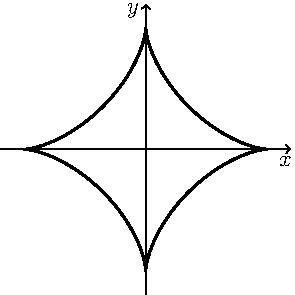
\includegraphics[width=5cm]{./img/Astroid.pdf}
		\caption{Астроида}
		\label{fig:Astroid}
	\end{figure}

	Приступим к решению задачи. Сначала посчитаем ориентированную кривизну по формуле \eqref{eq:OrientedCurvature}. Для этого найдём производные $\dot{\vec{r}}(t)$ (а она уже найдена) и $\ddot{\vec{r}}(t)$:
	\[
		\ddot{\vec{r}}(t) = 3a(2\cos t\sin^2t - \cos^3t, 2\cos^2t\sin t - \sin^3t).
	\]
	Теперь находим ориентированую площадь:
	\begin{multline*}
		S_{\Or}(\dot{\vec{r}}, \ddot{\vec{r}}) = a^2 \cdot \det
		\begin{pmatrix}
			-3\cos^2t\sin t & 3\sin^2t\cos t\\
			2\cos t\sin^2 t - \cos^3t & 2\cos^2t\sin t - \sin^3t
		\end{pmatrix} = \\ = a^2 \cdot (-6\cos^4t\sin^2t + 3\cos^2t\sin^4t - 6\cos^2t\sin^4t + 3\cos^4t\sin^2t) = -3a^2\sin^2t\cos^2t.
	\end{multline*}
	И, наконец, находим ориентированную кривизну:
	\[
		k_{\Or}(t) = \frac{-3a^2\sin^2t\cos^2t}{27a^3\cos^3t\sin^3t} = -\frac{1}{9a\cos t\sin t}.
	\]

	Мы хотим выразить $k_{\Or}$ через натуральный параметр, так что сначала надо найти натуральный параметр:
	\[
		s(t) = \int\limits_0^t\abs{\dot{\vec{r}}(t)}dt = 3a\int\limits_0^t\sin t\cos tdt = \frac{3a}{4}\int\limits_0^t\sin(2t) d(2t) = -\frac{3a}{4}\cos(2t).
	\]
	Итого получаем (здесь уже записываем через радиус кривизны $R = 1 / k$)
	\[
		R^2 = -9a^2\cos^2t\sin^2t = -\frac{9a^2}{4}\sin^2(2t) = \frac{9}{4}\cos^2t - \frac{9a^2}{4} = 4s^2 - \frac{9a^2}{4}.
	\]

	Отметим, что натуральное уравнение не единственное в том смысле, что можно брать натуральный параметр со сдвигом. Здесь, например, немного удобнее взять
	\[
		s(t) = -\frac{3a}{4}\cos(2t) + \frac{3a}{4}.
	\]
	(Это обусловлено тем, что теперь $s(0) = 0$.) Новое уравнение будет выглядеть так:
	\[
		R^2 - 6as - 4s^2 = 0.
	\]
	(Именно в такой форме ответ приведён в задачнике. Алгебраически мы могли его получить просто выделив полный квадрат в старом выражении.)
\end{solution}

В пространстве помимо векторов скорости $\vec{v} \vcentcolon = \dot{\vec{r}}$ и главной нормали $\vec{n} \vcentcolon = \ddot{\vec{r}} / \abs{\ddot{\vec{r}}}$ определяется \textit{вектор бинормали} $\vec{b} \vcentcolon = \vec{v} \times \vec{n}$.

\begin{definition}
	Точку $\vec{r}(s)$ и приложенный к ней базис $(\vec{v}(s), \vec{n}(s), \vec{b}(s))$ называют \textit{репером Френе} пространственной кривой.
\end{definition}

Для этого репера есть аналоги формул \eqref{eq:PlaneFrenet}.

\begin{theorem}[\textit{Формулы Френе для пространственных кривых}]
	Для пространственных кривых выполнено
	\begin{equation} \label{eq:SpaceFrenet}
		\begin{pmatrix}
			\dot{\vec{v}}(s) & \dot{\vec{n}}(s) & \dot{\vec{b}}(s)
		\end{pmatrix} = 
		\begin{pmatrix}
			\vec{v}(s) & \vec{n}(s) & \vec{b}(s)
		\end{pmatrix}
		\begin{pmatrix}
			0 & -k(s) & 0 \\
			k(s) & 0 & -\varkappa(s) \\
			0 & \varkappa(s) & 0
		\end{pmatrix},
	\end{equation}
	где $\varkappa(s)$ --- некоторая гладкая функция.
\end{theorem}

\begin{proof}
	Аналогично формулам для плоских кривых, $\dot{\vec{v}} = k\vec{n}$. Из определения, $\abs{\vec{n}} = 1$, значит, $\vec{n} \perp \dot{\vec{n}}$, так что $\dot{\vec{n}} = \alpha\vec{v} + \beta\vec{b}$. Здесь $\alpha = \langle\vec{v}, \dot{\vec{n}}\rangle = -\langle\dot{\vec{v}}, \vec{n}\rangle = -k$, $\beta = \langle\dot{\vec{n}}, \vec{b}\rangle$. $\abs{\vec{b}} = \abs{\vec{v} \times \vec{n}} = 1$, значит, $\dot{\vec{b}} \perp \vec{b}$, отсюда $\dot{\vec{b}} = \alpha\vec{v} + \beta\vec{n}$. Находим коэффициенты: $\alpha = \langle \dot{\vec{b}}, \vec{v} \rangle \hm= -\langle\vec{b}, \dot{\vec{v}}\rangle = 0$, $\beta = \langle\dot{\vec{b}}, \vec{n}\rangle = -\langle \vec{b}, \dot{\vec{n}}\rangle$. Обозначив $\varkappa \vcentcolon = \langle\dot{\vec{n}}, \vec{b}\rangle$, получим формулы \eqref{eq:SpaceFrenet}.
\end{proof}

Геометрический смысл кручения виден из третьего уравнения в \eqref{eq:SpaceFrenet}: это скорость вращения соприкасающейся плоскости кривой в данной точке. Выведем удобную формулу для кручения в натуральной параметризации:
\[
	\dot{\vec{r}} = \vec{v},\quad \ddot{\vec{r}} = \dot{\vec{v}} = k\vec{n},\quad \dddot{\vec{r}} = \frac{d}{ds}(k\vec{n}) = \dot{k}\vec{n} + k\dot{\vec{n}} = \dot{k}\vec{n} - k^2\vec{v} + \varkappa k\vec{b}.
\]
Заметим, что
\[
	\Vol_{\Or}(\dot{\vec{r}}, \ddot{\vec{r}}, \dddot{\vec{r}}) = \Vol_{\Or}(\vec{v}, k\vec{n}, \varkappa k\vec{b}) = k^2\varkappa \underbrace{\Vol_{\Or}(\vec{v}, \vec{n}, \vec{b})}_1 = k^2\varkappa.
\]

Отсюда, $\varkappa(s) = \Vol_{\Or}(\dot{\vec{r}}(s), \ddot{\vec{r}}(s), \dddot{\vec{r}}(s)) / k(s)^2$. Теперь перейдём в произвольную параметризацию. Для этого нужно будет выразить производные по $s$ через производные по $t$, как мы это делали при выводе формулы \eqref{eq:CurvatureFormula}:
\[
	\dot{\vec{r}}(s) = \frac{\vec{r}^\prime(t)}{\abs{\vec{r}^\prime(t)}},\quad \ddot{\vec{r}}(s) = \frac{\vec{r}^{\prime\prime}(t)}{\abs{\vec{r}^\prime(t)}^2}+ \ldots,\quad \dddot{\vec{r}}(s) = \frac{\vec{r}^{\prime\prime\prime}(t)}{\abs{\vec{r}^\prime(t)}^3} + \ldots
\]
Подставляем в формулу для натуральной параметризации:
\begin{multline} \label{eq:TorsionFormula}
	\varkappa(t) = \frac{1}{k^2}\Vol_{\Or}(\dot{\vec{r}}, \ddot{\vec{r}}, \dddot{\vec{r}}) = \frac{\cancel{\abs{\vec{r}^\prime(t)}^6}}{S^2_{\Or}(\vec{r}^\prime(t), \vec{r}^{\prime\prime}(t))} \cdot \frac{1}{\cancel{\abs{\vec{r}^\prime(t)}^6}}\Vol_{\Or}(\vec{r}^\prime(t), \vec{r}^{\prime\prime}(t), \vec{r}^{\prime\prime\prime}(t)) =\\ = \frac{\Vol_{\Or}(\vec{r}^\prime(t), \vec{r}^{\prime\prime}(t), \vec{r}^{\prime\prime\prime}(t))}{S^2_{\Or}(\vec{r}^\prime(t), \vec{r}^{\prime\prime}(t))}.
\end{multline}

Отметим, что из доказательства последней формулы видно, что базис Френе получается из базиса $(\vec{r}^\prime(t), \vec{r}^{\prime\prime}(t), \vec{r}^{\prime\prime\prime}(t))$, который пишется в произвольной параметризации, ортогонализацией Грама "---Шмидта (что, впрочем, верно и в плоском случае).

\noindent
Формулы Френе для пространственной кривой можно записать несколько более элегантно.

\begin{definition}
	\textit{Вектором Дарбу} $\vec{w}(s)$ называется вектор вдоль кривой, с помощью которого уравнения Френе могут быть записаны в следующем виде:
	\[
		\begin{cases}
			\dot{\vec{v}}(s) = \vec{w}(s) \times \vec{v}(s),\\
			\dot{\vec{n}}(s) = \vec{w}(s) \times \vec{n}(s),\\
			\dot{\vec{b}}(s) = \vec{w}(s) \times \vec{b}(s).
		\end{cases}
	\]
\end{definition}

\begin{theorem}
	Вектор Дарбу существует и единственен в каждой точке.
\end{theorem}

\begin{proof}
	Предположим, что такой вектор существует, тогда разложим его по базису Френе $\vec{w} = \alpha\vec{v} + \beta\vec{n} + \gamma\vec{b}$ и подставим в первое уравнение:
	\[
		\dot{\vec{v}} = (\alpha\vec{v} + \beta\vec{n} + \gamma\vec{b}) \times \vec{v} = -\beta\vec{b} + \gamma\vec{n}.
	\]
	С другой стороны, выполнены уравнения Френе, откуда следует, что $\beta \equiv 0$ и $\gamma \equiv k$, то есть $\vec{w} = \alpha\vec{v} + k\vec{b}$. Теперь подставим во второе уравнение:
	\[
		\dot{\vec{n}} = (\alpha\vec{v} + k\vec{b}) \times \vec{n} = \alpha\vec{b} - k\vec{v}.
	\]
	Аналогично из уравнений Френе получаем $\alpha \equiv \varkappa$. Отсюда $\vec{w} = \varkappa\vec{v} + k\vec{b}$. Осталось проверить выполнение третьего уравнения для такого вектора:
	\[
		\dot{\vec{b}} = (\varkappa\vec{v} + k\vec{b}) \times \vec{b} = -\varkappa\vec{n},
	\]
	что соответствует третьему уравнению Френе. Таким образом, вектор Дарбу существует и определён однозначно.
\end{proof}

Геометрический смысл вектора Дарбу заключается в том, что это направляющий вектор мгновенной оси вращения репера Френе при движении вдоль кривой, а его длина есть угловая скорость этого вращения.

\begin{proposition}
	Бирегулярная кривая является плоской тогда и только тогда, когда $\varkappa = 0$ (в каждой точке).
\end{proposition}

\begin{proof}
	Легко видеть, что кривая плоская тогда и только тогда, когда $\vec{b}(s) \hm= \vec{v}(s) \times \vec{n}(s) = \const$. Действительно, вектор $\vec{b}$ является просто единичной нормалью плоскости, в которой лежит кривая. А третья формула из \eqref{eq:SpaceFrenet} влечёт, что $\vec{b} = \const$, если и только если $\varkappa = 0$.
\end{proof}

Формулы Френе имеют важное следствие. Если в плоском случае мы восстанавливали коориентированную кривую по гладкой функции ориентированной кривизны, то здесь нам нужно знать гладкие функции кривизны и кручения.

\begin{theorem} \label{theorem:FundamentalSpaceCurves}
	Для любой пары гладких функций $k, \varkappa\colon I \to \R$, первая из которых всюду положительна, с точностью до движения существует ровно одна кривая в $\R^3$, кривизна и кручение которой выражаются для некоторой натуральной параметризации функциями $k$ и $\varkappa$ соответственно.
\end{theorem}

\begin{proof}
	Доказательство единственности не отличается от плоского случая. Уравнения \eqref{eq:SpaceFrenet} вместе с $\vec{r}^\prime = \vec{v}$ образуют систему обыкновенных дифференциальных уравнений, решение которой единственно при фиксированных начальных условиях, которыми являются начальная точка и базис Френе в начальный момент. Любой ортонормированный положительно ориентированный репер переводится движением в любой другой. Поэтому начальные данные одного решения можно перевести в начальные данные другого решения. При этом одно решение перейдёт в другое в силу инвариантности уравнений относительно группы собственных движений.

	Для доказательства существования нужно взять произвольный начальный момент $s_0 \in I$ и произвольный ортонормированный положительно ориентированный репер: $\vec{x}_0$, $\vec{v}_0$, $\vec{n}_0$, $\vec{b}_0$, решить уравнения \eqref{eq:SpaceFrenet}, а затем уравнение $\vec{r}^\prime = \vec{v}$ с начальными условиями $\vec{r}(s_0) = \vec{x}_0$, $\vec{v}(s_0) = \vec{v}_0$, $\vec{n}(s_0) = \vec{n}_0$, $\vec{b}(s_0) = \vec{b}_0$. Решение существует на всём промежутке $I$ (а не только в малой окрестности точки фазового пространства, заданной начальными условиями), поскольку уравнения линейны. Нужно лишь проверить, что кривизна и кручение полученной кривой действительно выражаются исходными функциями $k(s)$, $\varkappa(s)$. Для этого достаточно показать, что базис $(\vec{v}, \vec{n}, \vec{b})$ остаётся ортонормированным в силу уравнений \eqref{eq:SpaceFrenet}.

	\begin{lemma} \label{lemma:FunnyMatrixLemma}
		Пусть $X(t)$ --- матрица $n \times n$, гладко зависящая от параметра, причём в начальный момент $t = 0$ она ортогональна. Тогда матрица $X(t)$ ортогональна при всех $t$ тогда и только тогда, когда $X^{-1}(t)\dot{X}(t)$ кососимметрична при всех $t$.
	\end{lemma}

	\begin{proof}
		Положим $A(t) \vcentcolon = X^t(t)X(t)$, $B(t) \vcentcolon = X^{-1}(t)\dot{X}(t)$ (здесь, конечно же, через $X^t$ обозначается не степень, а транспонирование). Имеем
		\begin{equation} \label{eq:dotA}
			\dot{A} = \dot{X}^t X + X^t\dot{X} = B^t A + AB.
		\end{equation}
		Матрица $X(t)$ ортогональна тогда и только тогда, когда $A(t) = E$. Если $A(t) = E$ для всех $t$, то из \eqref{eq:dotA} следует, что $B^t(t) + B(t) = 0$ для всех $t$. Пусть, наоборот, $B(t)$ кососимметрична (то есть $B^t(t) + B(t) = 0$) при всех $t$ и $A(0) = E$. Тогда постоянная функция $A(t) = E$ является решением уравнения \eqref{eq:dotA} с этим начальным условием. Остаётся воспользоваться единственностью решения.
	\end{proof}

	Вернёмся к доказательству. Обозначим
	\[
		A(s) = \begin{pmatrix}
			\vec{v}(s) & \vec{n}(s) & \vec{b}(s)
		\end{pmatrix},
	\]
	где $\vec{v}$, $\vec{n}$, $\vec{b}$ найдены из \eqref{eq:SpaceFrenet}. Ортонормированность базиса $(\vec{v}, \vec{n}, \vec{b})$ означает ортогональность матрицы $A(s)$. В начальный момент $s = s_0$ условие ортогональности выполнено. Уравнения \eqref{eq:SpaceFrenet} переписываются в виде
	\[
		\dot{A} = A
		\begin{pmatrix}
			0 & -k & 0\\
			k & 0 & -\varkappa\\
			0 & \varkappa & 0
		\end{pmatrix}.
	\]
	Отсюда по лемме \ref{lemma:FunnyMatrixLemma} матрица $A(s)$ ортогональна при всех $s$.
\end{proof}


\begin{problem}
	Дана кривая $\vec{r}(t) = (\ch t, \sh t, t)$.
	\begin{enumerate}[nolistsep, label=(\arabic*)]
		\item Привести её к натуральному параметру.
		\item Найти репер Френе в каждой точке.
		\item Найти кривизну и кручение в каждой точке.
	\end{enumerate}
\end{problem}

\begin{solution}
	У этой кривой легко пишутся производные всех порядков:
	\begin{gather*}
		\dot{\vec{r}}(t) = (\sh t, \ch t, 1),\\
		\ddot{\vec{r}}(t) = (\ch t, \sh t, 0),\\
		\dddot{\vec{r}}(t) = (\sh t, \ch t, 0).
	\end{gather*}
	\begin{enumerate}[nolistsep, label=(\arabic*)]
		\item Ищем натуральный параметр по формуле длины кривой:
			\[
				s(t) = \int\limits_0^t\abs{\dot{\vec{r}}(t)}dt = \int\limits_0^t\sqrt{\sh^2t + \ch^2t + 1}dt = \sqrt{2}\int\limits_0^t\ch t\,dt = \sh t\sqrt{2}.
			\]
			Теперь надо каждую координату вектора $\vec{r}(t)$ выразить через натуральный параметр. Для первых двух координат это делается совсем тривиально, а для третьей надо решить квадратное уравнение относительно $e^t$:
			\begin{gather*}
				s = \sqrt{2} \cdot \frac{e^t - e^{-t}}{2},\\
				e^{2t} - s\sqrt{2} \cdot e^t - 1 = 0,\\
				e^t = \frac{s\sqrt{2} + \sqrt{2s^2 + 4}}{2} = \frac{s}{\sqrt{2}} + \sqrt{s^2 + 2},\\
				t = \ln\br{\frac{s}{\sqrt{2}} + \sqrt{s^2 + 2}}.
			\end{gather*}
			Здесь выбрали положительный корень квадратного уравнения, так как $e^t > 0$ для всех $t$. Итого, получаем
			\[
				\vec{r}(s) = \br{\frac{s}{\sqrt{2}}, \sqrt{s^2 + 2}, \ln\br{\frac{s}{\sqrt{2}} + \sqrt{s^2 + 2}}}.
			\]
		\item Воспользуемся ортогонализацией Грама "---Шмидта:
			\[
				\vec{v}(t) = \frac{\dot{\vec{r}}(t)}{\abs{\dot{\vec{r}}(t)}} = \frac{1}{\sqrt{2}\ch t}(\sh t, \ch t, 1) = \frac{1}{\sqrt{2}}\br{\th t, 1, \frac{1}{\ch t}},
			\]
			теперь найдём вектор, совпадающий по направлению с $\vec{n}(t)$:
			\[
				\ddot{\vec{r}}(t) - \frac{\langle \vec{v}(t), \ddot{\vec{r}}(t) \rangle}{\langle \vec{v}(t), \vec{v}(t)\rangle}\vec{v}(t) = (\ch t, \sh t, 0) - \cancel{\sqrt{2}}\sh t \cdot \frac{1}{\cancel{\sqrt{2}}}\br{\th t, 1, \frac{1}{\ch t}} = \br{\frac{1}{\ch t}, 0, -\th t}.
			\]
			Осталось его нормировать, для этого вычислим квадрат его длины:
			\[
				\frac{1}{\ch^2t} + \th^2t = \frac{1 + \sh^2t}{\ch^2t} = 1.
			\]
			Таким образом, нормировать ничего не надо, и $\vec{n}(t) = (1 / \ch t, 0, -\th t)$. Осталось только найти вектор бинормали, это проще делать уже не по Граму "---Шмидту, а просто по определению:
			\[
				\vec{b} = \vec{v} \times \vec{n} = \frac{1}{\sqrt{2}}\det
				\begin{pmatrix}
					\vec{e}_1 & \vec{e}_2 & \vec{e}_3\\
					\th t & 1 & \frac{1}{\ch t}\\
					\frac{1}{\ch t} & 0 & -\th t
				\end{pmatrix} = \frac{1}{\sqrt{2}}\br{-\th t, 1, -\frac{1}{\ch t}}.
			\]
		\item Так как мы уже нашли репер Френе, нам проще не пользоваться формулами \eqref{eq:CurvatureFormula} и \eqref{eq:TorsionFormula} (и тем более не расписывать через натуральный параметр), а исходить из формул Френе. Мы знаем, что $\dot{\vec{v}} = k\vec{n}$, тогда можно просто <<подобрать>> коэффициент пропорциональности между нужными векторами.
			\[
				\dot{\vec{v}}(t) = \frac{1}{\sqrt{2}}\br{\frac{1}{\ch^2t}, 0, -\frac{\sh t}{\ch^2t}} = k(t) \cdot \br{\frac{1}{\ch t}, 0, -\th t}.
			\]
			Отсюда сразу видно, что $k(t) = 1 / (\ch t\sqrt{2})$. Можно так же поступить и для кручения, ведь мы знаем, что $\dot{\vec{b}} = -\varkappa\vec{n}$:
			\[
				\dot{\vec{b}}(t) = \frac{1}{\sqrt{2}}\br{-\frac{1}{\ch^2t}, 0, \frac{\sh t}{\ch^2t}} = -\varkappa(t) \cdot \br{\frac{1}{\ch t}, 0, -\th t}.
			\]
			Получаем $\varkappa(t) = 1 / (\ch t\sqrt{2})$.
	\end{enumerate}
\end{solution}

Решим задачу нахождения кривизны и кручения кривой, которая задана не параметрически, а системой уравнений.

\begin{problem}
	Найти кривизну и кручение кривой, заданной уравнениями
	\[
		\begin{cases}
			x^2 + z^2 - y^2 = 1,\\
			y^2 - 2x + z = 0
		\end{cases}
	\]
	в точке $(1, 1, 1)$.
\end{problem}

\begin{solution}
	Сначала проверим, что в окрестности этой точки пересечение данных поверхностей действительно представляет собой гладкую кривую. Для этого, согласно теореме \ref{theorem:SurfacesToCurve}, достаточно проверить, что точка $(1, 1, 1)$ является регулярной для отображения $\vec{f} = (f_1, f_2)$, где $f_1(x, y, z) = x^2 - y^2 + z^2 - 1$, $f_2(x, y, z) = -2x + y^2 + z$.
	\begin{gather*}
		\left.\grad f_1\right|_{(1, 1, 1)} = \left.(2x, -2y, 2z)\right|_{(1, 1, 1)} = (2, -2, 2),\\
		\left.\grad f_2\right|_{(1, 1, 1)} = \left.(-2, 2y, 1)\right|_{(1, 1, 1)} = (-2, 2, 1).
	\end{gather*}

	Видим, что градиенты в интересующих нас точках в самом деле линейно независимы, то есть $\rk J_{\vec{f}}(1, 1, 1) = 2$. Далее мы хотим явно параметризовать данную кривую в окрестности нашей точки. И мы уже знаем, что в качестве параметра нам точно подойдёт какая-то из координат (замечание после доказательства предложения \ref{proposition:SmoothHomeomorphism}), но важно точно понять, какая именно. Нужно посмотреть на матрицу Якоби (которая на самом деле уже выписана сверху) и увидеть два линейно независимых столбца. Подойдут, например, последние два, так что будем выражать переменные $y$ и $z$ через $x$. Целиком выразить $y$ и $z$ из данной нам системы можно, но проблематично. Тем более, позднее мы собираемся пользоваться формулами \eqref{eq:CurvatureFormula} и \eqref{eq:TorsionFormula}, так что нам нужно будет знать их производные вплоть до третьего порядка. Однако можно смотреть на это по-другому --- кроме первых трёх производных нам больше ничего не нужно, так что их и будем искать. Напишем ряды Тейлора с неопределёнными коэффициентами вблизи точки $x = 1$, но чтобы избавиться от обилия возникающих скобок, сделаем замену $\widetilde{x} = x - 1$:
	\begin{gather*}
		y(\widetilde{x}) = 1 + a_1\widetilde{x} + a_2\widetilde{x}^2 + a_3\widetilde{x}^3 + \o(\widetilde{x}^3),\\
		z(\widetilde{x}) = 1 + b_1\widetilde{x} + b_2\widetilde{x}^2 + b_3\widetilde{x}^3 + \o(\widetilde{x}^3).
	\end{gather*}

	Найдём коэффициенты подстановкой в данную нам систему. Для упрощения вычислений можно сложить два уравнения, получив новое уравнение
	\begin{gather*}
		x^2 + z^2 - 2x + z = 1,\\
		\br{x - 1}^2 + \br{z + \frac{1}{2}}^2 - \frac{9}{4} = 0,
	\end{gather*}
	которое связывает $z$ и $x$. В нём надо сделать нашу замену и подставить разложение $z(\widetilde{x})$:
	\begin{gather*}
		\br{z + \frac{1}{2}}^2 = \frac{9}{4} - \widetilde{x}^2,\\
		\br{\frac{3}{2} + b_1\widetilde{x} + b_2\widetilde{x}^2 + b_3\widetilde{x}^3 + \o(\widetilde{x}^3)}^2 = \frac{9}{4} - \widetilde{x}^2.
	\end{gather*}
	
	Раскрываем скобки, отбрасывая члены порядка малости $\o(\widetilde{x}^3)$, и пишем систему на равенство коэффициентов получившихся многочленов в левой и правой части:
	\[
		\begin{cases}
			3b_3 + 2b_1b_2 = 0,\\
			b_1^2 + 3b_2 = -1,\\
			3b_1 = 0.
		\end{cases}
	\]

	Отсюда получаем $b_1 = 0$, $b_2 = -\frac{1}{3}$, $b_3 = 0$. Подставляя, получаем $z(\widetilde{x}) = 1 - \frac{1}{3}\widetilde{x}^2 + \o(\widetilde{x}^3)$. Теперь можем подставить найденное во второе уравнение системы и выразить $y(\widetilde{x})$.
	\begin{gather*}
		\br{1 + a_1\widetilde{x} + a_2\widetilde{x}^2 + a_3\widetilde{x}^3 + \o(\widetilde{x}^3)}^2 - 2(\widetilde{x} + 1) + 1 - \frac{1}{3}\widetilde{x}^2 = 0,\\
		\br{1 + a_1\widetilde{x} + a_2\widetilde{x}^2 + a_3\widetilde{x}^3 + \o(\widetilde{x}^3)}^2 = 1 + 2\widetilde{x} + \frac{1}{3}\widetilde{x}^2.
	\end{gather*}
	Получаем систему:
	\[
		\begin{cases}
			2a_3 + 2a_1a_2 = 0,\\
			a_1^2 + 2a_2 = \frac{1}{3},\\
			2a_1 = 2.
		\end{cases}
	\]

	Отсюда $a_1 = 1$, $a_2 = -\frac{1}{3}$, $a_3 = \frac{1}{3}$. Таким образом, $y(\widetilde{x}) = 1 + \widetilde{x} - \frac{1}{3}\widetilde{x}^2 + \frac{1}{3}\widetilde{x}^3 + \o(\widetilde{x}^3)$. Теперь совершим обратную замену:
	\begin{gather*}
		y(x) = 1 + (x - 1) - \frac{1}{3}(x - 1)^2 + \frac{1}{3}(x - 1)^3 + \o((x - 1)^3),\\
		z(x) = 1 - \frac{1}{3}(x - 1)^2 + \o((x - 1)^3).
	\end{gather*}
	
	Из найденного разложения находим: $y^\prime(1) = 1$, $y^{\prime\prime}(1) = -\frac{1}{3} \cdot 2! = -\frac{2}{3}$, $y^{\prime\prime\prime}(1) = \frac{1}{3} \cdot 3! = 2$ и $z^\prime(1) = 0$, $z^{\prime\prime}(1) = -\frac{1}{3} \cdot 2! = -\frac{2}{3}$, $z^{\prime\prime\prime}(1) = 0$. По формуле кривизны \eqref{eq:CurvatureFormula} имеем
	\[
		k(1) = \frac{\abs{(1, 1, 0) \times (0, -\frac{2}{3}, -\frac{2}{3})}}{\abs{(1, 1, 0)}^3} = \frac{1}{\sqrt{6}}.
	\]
	А по формуле кручения \eqref{eq:TorsionFormula}
	\[
		\varkappa(1) = \frac{\Vol_{\Or}\br{(1, 1, 0), (0, -\frac{2}{3}, -\frac{2}{3}), (0, 2, 0)}}{\abs{(1, 1, 0) \times (0, -\frac{2}{3}, -\frac{2}{3})}^2} = 1.
	\]
\end{solution}

\subsection{Эволюта и эвольвента плоской кривой \label{section:EvoluteInvolute}}

\begin{definition}
	\textit{Эволютой} плоской бирегулярной кривой $\gamma$ называется кривая, которую описывает центр кривизны кривой $\gamma$.
\end{definition}

Пусть $\vec{r}(s)$ --- натуральная параметризация кривой $\gamma$, тогда имеем параметризацию (уже не обязательно натуральную) эволюты:
\begin{equation} \label{eq:Evolute}
	\widetilde{\vec{r}}(s) = \vec{r}(s) + \frac{1}{k(s)}\vec{n}(s).
\end{equation}

\begin{proposition} \label{proposition:NormalEnvelope}
	Кривая $\widetilde{\gamma}$ является эволютой плоской бирегулярной кривой $\gamma$ тогда и только тогда, когда $\widetilde{\gamma}$ является огибающей семейства нормалей к $\gamma$.
\end{proposition}

\begin{proof}
	Пусть $\vec{r}(s)$ --- натуральная параметризация кривой $\gamma$.

	$\Rightarrow$. Параметризация эволюты $\widetilde{\gamma}$ имеет вид \eqref{eq:Evolute}. В каждой точке можем вычислить вектор скорости:\footnotemark
	\[
		\widetilde{\vec{r}}^\prime = \dot{\vec{r}} + \frac{1}{k}\dot{\vec{n}} - \frac{k^\prime}{k^2}\vec{n} = -\frac{k^\prime}{k^2}\vec{n},
	\]
	что и требовалось. (Во втором равенстве воспользовались формулой Френе для плоской кривой $\gamma$.)

	$\Leftarrow$. Можем записать параметризацию $\widetilde{\gamma}$ в виде
	\[
		\widetilde{\vec{r}}(s) = \vec{r}(s) + \lambda(s)\vec{n}(s).
	\]

	Кривая $\widetilde{\gamma}$ является огибающей поля нормалей к $\gamma$. Это значит, что в каждой точке $s$ вектор скорости $\widetilde{\vec{r}}^\prime(s)$ кривой $\widetilde{\gamma}$ должен быть коллинеарен вектору главной нормали $\vec{n}(s)$ кривой $\gamma$, это задаёт условие на коэффициент $\lambda$:
	\[
		\widetilde{\vec{r}}^\prime = (1 - k\lambda)\vec{v} + \lambda^\prime\vec{n}.
	\]
	Отсюда сразу получаем $\lambda = 1 / k$, что и требовалось.
\end{proof}

\footnotetext{Здесь производные берутся по одному и тому же параметру $s$, но обозначены по-разному (точками и штрихами), потому что для кривой $\gamma$ этот параметр натуральный, а для кривой $\widetilde{\gamma}$ --- нет.}

\begin{theorem}[Тейт, Кнезер]
	Если на кривизна кривой является строго монотонной функцией, то соприкасающиеся окружности вложены друг в друга.
\end{theorem}

\begin{proof}
	Пусть $\vec{r}(s)$ --- натуральная параметризация данной кривой. Положим, для определённости, $k^\prime > 0$. Возьмём произвольные значения параметра $s_0$, $s_1$ ($s_0 < s_1$) и докажем, что соприкасающаяся окружность в точке $\vec{r}(s_1)$ вложена в соприкасающуюся окружность в точке $\vec{r}(s_0)$. Длина участка эволюты, заключённого между центрами соприкасающихся окружностей в данных точка, равна
	\[
		\int\limits_{s_0}^{s_1}\abs{\widetilde{\vec{r}}^\prime(s)}\,ds = \int\limits_{s_0}^{s_1}\frac{k^\prime}{k^2}\,ds = \left.\br{-\frac{1}{k(s)}}\right|_{s_0}^{s_1} = \frac{1}{k(s_0)} - \frac{1}{k(s_1)}.
	\]
	Отметим, что эта величина есть разность радиусов соприкасающихся окружностей в точках $\vec{r}(s_0)$ и $\vec{r}(s_1)$. Но тогда расстояние между центрами окружностей не больше разности их радиусов, а значит, одна из них лежит внутри другой. (Ясно, что внутри лежит окружность меньшего радиуса.)
\end{proof}

\begin{definition}
	\textit{Эвольвентой} плоской бирегулярной кривой $\gamma$ называется кривая, которую описывает неподвижная точка прямой, катящейся без проскальзывания по $\gamma$.
\end{definition}

Эвольвента (в отличие от эволюты) не определена однозначно, ведь можно выбрать любую точку на катящейся прямой. Так что у бирегулярной плоской кривой имеется однопараметрическое семейство эвольвент. Если $\vec{r}(s)$ --- натуральная параметризация кривой $\gamma$, то легко получить (опять же, необязательно натуральную) параметризацию эвольвенты:
\begin{equation} \label{eq:Involute}
	\widehat{\vec{r}}(s) = \vec{r}(s) - (s - s_0)\dot{\vec{r}}(s).
\end{equation}

Константа $s_0$ как раз соответствует изначальному смещению точки по скользящей прямой, её выбор соответствует выбору эвольвенты.

\begin{theorem}
	Пусть $\gamma$ и $\widehat{\gamma}$ --- регулярные кривые. Следующие условия равносильны:
	\begin{enumerate}[nolistsep, label=(\arabic*)]
		\item кривая $\widehat{\gamma}$ является эвольвентой кривой $\gamma$;
		\item кривая $\gamma$ является огибающей поля нормалей к $\widehat{\gamma}$;
		\item кривая $\gamma$ является эволютой кривой $\widehat{\gamma}$.
	\end{enumerate}
\end{theorem}

\begin{proof}
	Пусть $\vec{r}(s)$ --- регулярная параметризация кривой $\gamma$.

	$(1) \Rightarrow (2)$. Кривая $\widehat{\gamma}$ имеет параметризацию \eqref{eq:Involute}. Вычисляем вектор скорости:
	\[
		\widehat{\vec{r}}^\prime = \cancel{\dot{\vec{r}}} - \cancel{\dot{\vec{r}}} - (s - s_0)\ddot{\vec{r}}
	\]
	и видим, что он перпендикулярен вектору $\dot{\vec{r}}$.

	$(2) \Leftarrow (1)$. Если кривая $\widehat{\gamma}$ ортогональна касательным к $\gamma$, то её параметризация имеет вид $\widehat{\vec{r}}(s) = \vec{r}(s) + \lambda(s)\dot{\vec{r}}(s)$. При этом должно быть выполнено $\langle\widehat{\vec{r}}^\prime, \dot{\vec{r}}\rangle = 0$:
	\[
		0 = \langle (1 + \lambda^\prime)\dot{\vec{r}} + \lambda\ddot{\vec{r}}, \dot{\vec{r}}\rangle = 1 + \lambda^\prime.
	\]
	Отсюда $\lambda(s) = -(s - s_0)$, то есть данная кривая является эвольвентой кривой $\gamma$.

	$(2) \Leftrightarrow (3)$. См. предложение \ref{proposition:NormalEnvelope}.
\end{proof}

%\subsection{Дополнительные задачи}
%
%Здесь собраны задачи, которые показались мне интересными, но не вписались в основное повествование. Какие-то из них я умею решать, какие-то нет. Так или иначе, я надеюсь когда-нибудь написать сюда все решения.
%
%\begin{problem}
%	Пусть $\vec{r}(s)$ --- натуральная параметризация бирегулярной кривой $\gamma$ в $\R^3$ с ненулевым кручением. Кривая $\gamma$ лежит на сфере тогда и только тогда, когда
%	\[
%		\frac{\varkappa}{k} = \frac{d}{ds}\br{\frac{dk / ds}{\varkappa k^2}}.
%	\]
%\end{problem}
%
%\begin{problem}
%	Построить гладкую замкнутую плоскую кривую с числом вращения $0$.
%\end{problem}
%
%\begin{problem}
%	Доказать, что для замкнутой регулярной кривой в $\R^3$ выполняется
%	\[
%		\oint\limits_{\gamma}k(s)ds \geqslant 2\pi.
%	\]
%\end{problem}
%
%\begin{problem}
%	Пусть $\gamma$ --- гладкая регулярная замкнутая кривая. Доказать, что
%	\[
%		\oint\limits_{\gamma}(\vec{r}\,dk + \varkappa\vec{b}\,ds) = \vec{0}.
%	\]
%\end{problem}
%
%\begin{problem}
%	\textit{Вершинами} кривой называются точки этой кривой, в которых $k^\prime(s) = 0$. Доказать, что у любой замкнутой регулярной кривой есть по крайней мере четыре вершины.
%\end{problem}

\subsection{Кривые в $\R^n$}

\begin{definition}
	Кривая в евклидовом пространстве $\R^n$ называется \textit{$k$-регулярной}, если она допускает параметризацию $\vec{r}(t)$, для которой векторы
	\[
		\frac{d\vec{r}}{dt},\quad\frac{d^2\vec{r}}{dt^2},\quad\ldots,\quad \frac{d^k\vec{r}}{dt^k}
	\]
	линейно независимы при всех $t$.
\end{definition}

\begin{lemma} \label{lemma:UpperTriangleLemma}
	Пусть $t$ и $\tau$ --- два регулярных параметра на регулярной кривой $\gamma$. Тогда для любого $k \in \N$ в каждой точке кривой выполнено равенство
	\[
		\begin{pmatrix}
			\cfrac{d\vec{r}}{d\tau} & \cfrac{d^2\vec{r}}{d\tau^2} & \cdots & \cfrac{d^k\vec{r}}{d\tau^k}
		\end{pmatrix} =
		\begin{pmatrix}
			\cfrac{d\vec{r}}{dt} & \cfrac{d^2\vec{r}}{dt^2} & \cdots & \cfrac{d^k\vec{r}}{dt^k}
		\end{pmatrix} \cdot R,
	\]
	где $R$ --- верхнетреугольная матрица, на диагонали которой стоят числа
	\[
		\frac{dt}{d\tau},\quad\br{\frac{dt}{d\tau}}^2,\quad\cdots,\quad\br{\frac{dt}{d\tau}}^k.
	\]
\end{lemma}

\begin{proof}
	Мы хотим доказать, что для всех $j \in \N$ вектор $d^j\vec{r} / d\tau^j$ имеет вид
	\begin{equation} \label{eq:djdtauj}
		\frac{d^j\vec{r}}{d\tau^j} = \br{\frac{dt}{d\tau}}^j\frac{d^j\vec{r}}{dt^j} + R_{j - 1, j}\frac{d^{j - 1}\vec{r}}{dt^{j - 1}} + \ldots + R_{1, j}\frac{d\vec{r}}{dt},
	\end{equation}
	где $R_{j - 1, j}, \ldots, R_{1, j}$ --- некоторые коэффициенты. Будем доказывать по индукции. Для $j = 1$ равенство \eqref{eq:djdtauj} следует из теоремы о дифференцировании сложной функции. Для индукционного перехода продифференцируем обе части \eqref{eq:djdtauj} по $\tau$:
	\begin{multline*}
		\frac{d^{j + 1}\vec{r}}{d\tau^{j + 1}} = \br{\frac{dt}{d\tau}}^{j + 1}\frac{d^{j + 1}\vec{r}}{{dt^{j + 1}}} + \br{\frac{d}{d\tau}\br{\frac{dt}{d\tau}}^j + R_{j - 1, j}\frac{dt}{d\tau}}\frac{d^j\vec{r}}{dt^j} + {}\\ + \br{\frac{dR_{j - 1, j}}{d\tau} + R_{j - 2, j}\frac{dt}{d\tau}}\frac{d^{j - 1}\vec{r}}{dt^{j - 1}} + \ldots + \br{\frac{dR_{2, j}}{d\tau} + R_{1, j}\frac{dt}{d\tau}}\frac{d^2\vec{r}}{dt^2} + \frac{dR_{1, j}}{d\tau}\frac{d\vec{r}}{dt}.
	\end{multline*}
\end{proof}

Из последней леммы вытекает, что $k$-регулярность кривой не зависит от выбора регулярного параметра на ней.

\begin{definition}
	Пусть $\gamma$ --- $(n - 1)$-регулярная кривая в евклидовом пространстве $\R^n$ и $\vec{r}(t)$ --- её регулярная параметризация. Для каждой точки этой кривой её \textit{базисом Френе} в этой точке называется ортонормированный базис, в котором первые $n - 1$ векторов получены ортогонализацией Грама "---Шмидта из набора векторов
	\[
		\frac{d\vec{r}}{dt},\quad\frac{d^2\vec{r}}{dt^2},\quad\ldots,\quad \frac{d^{n - 1}\vec{r}}{dt^{n - 1}},
	\]
	а последний вектор выбран таким образом, чтобы ориентация базиса была положительной.
\end{definition}

Для начала докажем корректность определения репера Френе (то есть его независимость от параметризации).

\begin{proposition}
	Базис Френе гладкой ориентированной $(n - 1)$-регулярной кривой в $\R^n$ в каждой точке не зависит от выбора параметризации.
\end{proposition}

\begin{proof}
	Пусть $t$ и $\tau$ --- два одинаково ориентированных параметра на данной кривой, то есть $dt / d\tau > 0$, и пусть по отношению к обоим параметризация $\vec{r}$ данной кривой является регулярной.

	По лемме \ref{lemma:UpperTriangleLemma} матрицы перехода между базисами $(d^j\vec{r} / dt^j)_{j = 1, \ldots, {n - 1}}$ и $(d^j\vec{r} / d\tau^j)_{j = 1, \ldots, {n - 1}}$ верхнетреугольные с положительными элементами на диагонали. Так что результат процесса ортогонализации Грама "---Шмидта для них будет одинаковым. Последний вектор базиса Френе однозначно определяется остальными.
\end{proof}

\begin{theorem}
	Для базиса Френе $\vec{e}_1, \ldots, \vec{e}_n$ $n$-регулярной ориентированной кривой в $\R^n$, параметризованной натуральным параметром, имеют место равенства
	\[
		\begin{pmatrix}
			\dot{\vec{e}}_1 & \dot{\vec{e}}_2 & \ldots & \dot{\vec{e}}_n
		\end{pmatrix} =
		\begin{pmatrix}
			\vec{e}_1 & \vec{e}_2 & \ldots & \vec{e}_n
		\end{pmatrix}
		\begin{pmatrix}
			0 & -k_1 & & & & \\
			k_1 & 0 & -k_2 & & & \\
			 & k_2 & 0 & & & \\
			 & & & \ddots & & \\
			 & & & & 0 & -k_{n - 1}\\
			 & & & & k_{n - 1} & 0\\
		\end{pmatrix},
	\]
	где $k_1, \ldots, k_{n - 1}$ --- некоторые гладкие функции натурального параметра (они называются \textit{обобщёнными кривизнами} данной кривой).
\end{theorem}

\begin{proof}
	Будем доказывать утверждение с помощью индукции. Так как на кривой выбрана натуральная параметризация, первый вектор при ортогонализации не изменится: $\vec{e}_1 = \dot{\vec{r}}$. Вектор $\ddot{\vec{r}}$ уже перпендикулярен первому $\dot{\vec{r}}$, так что его останется только нормировать: $\vec{e}_2 = \ddot{\vec{r}} / \abs{\ddot{\vec{r}}}$. Далее будут возникать всё более сложные выражения, но нам важно, что для каждого $i$ вектор $\vec{e}_i$ выражается через векторы $\dot{\vec{r}}, \ldots, \vec{r}^{(i)}$ (это эквивалентно тому, что матрица замены при ортогонализации Грама "---Шмидта верхнетреугольная).

	Векторы $\vec{e}_1, \ldots, \vec{e}_n$ в каждой точке нашей кривой образуют ортонормированный базис, так что для каждого $s$ можем написать
	\[
		\begin{pmatrix}
			\vec{e}_1(s + t) & \vec{e}_2(s + t) & \ldots & \vec{e}_n(s + t)
		\end{pmatrix} =
		\begin{pmatrix}
			\vec{e}_1(s) & \vec{e}_2(s) & \ldots & \vec{e}_n(s)
		\end{pmatrix}A_s(t),
	\]
	где $A_s \in \mathrm{SO}(n)$. При $t = 0$ матрица $A_s$ единичная, так что по лемме \ref{lemma:FunnyMatrixLemma} матрица $A_s^{-1}A_s^\prime$ кососимметрична (здесь штрихом обозначена производная по $t$). При $t = 0$ получаем кососимметричность матрицы $A_s^\prime|_{t = 0}$. В последней формуле возьмём производную по $t$, а затем положим $t = 0$:
	\[
		\begin{pmatrix}
			\dot{\vec{e}_1}(s) & \dot{\vec{e}}_2(s) & \ldots & \dot{\vec{e}}_n(s)
		\end{pmatrix} =
		\begin{pmatrix}
			\vec{e}_1(s) & \vec{e}_2(s) & \ldots & \vec{e}_n(s)
		\end{pmatrix}B,
	\]
	где матрица $B \vcentcolon = A_s^\prime|_{t = 0}$ кососимметрична. Мы уже почти доказали теорему, осталось только понять, какой именно вид имеет матрица $B$.

	Как было сказано выше, $\vec{e}_i$ является линейной комбинацией векторов $\dot{\vec{r}}, \ldots, \vec{r}^{(i)}$, так что $\dot{\vec{e}}_i$ есть некоторая линейная комбинация $\dot{\vec{r}}, \ldots, \vec{r}^{(i + 1)}$. Отсюда можем заключить, что $\dot{\vec{e}}_i$ линейно выражается через $\vec{e}_1, \ldots, \vec{e}_{i + 1}$.

	Таким образом, ненулевыми в матрице $B$ могут быть только элементы, стоящие ровно на одну клетку выше или ниже главной диагонали, притом матрица $B$ кососимметрична. Это и есть утверждение, которое мы хотели доказать.
\end{proof}

Доказательство следующей теоремы в точности повторяет её доказательство для трёхмерного случая, поэтому заново его здесь писать мы не будем.

\begin{theorem}
	Пусть заданы гладкие функции $k_1(s) > 0, \ldots, k_{n - 2}(s) > 0, k_{n - 1}(s)$. Тогда существует единственная $(n - 1)$-регулярная кривая с точностью до движения пространства, для которых эти функции являются обобщёнными кривизнами.
\end{theorem}

\subsection{Про механические часы}

Фраза из эпиграфа связана с историей создания точных механических часов, рассказанной нам Александром Алексадровичем на семинаре.

\textit{Циклоидой} называется кривая, которую описывает неподвижная точка на окружности, движущейся по прямой без проскальзывания.

\begin{figure}[H]
	\centering
	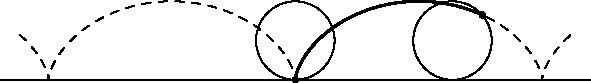
\includegraphics[width=12cm]{./img/Cycloid.pdf}
	\caption{Циклоида}
\end{figure}

В \rnum{17} веке голландский математик\footnotemark{} Х.\,Гюйгенс описал устройство точных механических часов, конструкция которых основана на маятнике, который обладает постоянным периодом качения независимо от амплитуды. Это действительно важное свойство --- период колебания маятника в часах не должен зависеть от силы, с которой заводят часы, или от эффекта постепенного затухания колебаний. Как же может быть устроен такой маятник? Оказывается, конец его нити должен вырисовывать перевёрнутую <<чашу циклоиды>>. Немного позже мы докажем, почему это действительно так, но сейчас зададимся вопросом, как же сделать такой \textit{циклоидный маятник}.

\footnotetext{Гюйгенс, конечно, был не только математиком, но ещё и физиком и философом, что, впрочем, не было исключением для того времени.}

Сначала выведем уравнение циклоиды. Примем за $t = 0$ момент времени, когда точка окружности, движение которой мы отслеживаем, находится на прямой, по которой катится эта окружность. Предположим также, что окружность единичная, а её центр движется равномерно на единицу расстояния за единицу времени. Ясно, что все эти допущения не влияют существенно на уравнения, которые мы будем получать.

\begin{figure}[H]
	\centering
	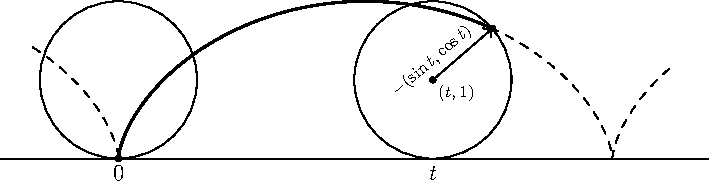
\includegraphics[width=12cm]{./img/CycloidEquation.pdf}
	\caption[format=empty]{}
\end{figure}

Центр окружности в момент времени $t$ находится в точке с координтами $(t, 1)$. Теперь представим, что окружность просто равномерно вращается с закреплённым центром. Тогда движение её граничной точки, конечно, будет описываться вектором $-(\sin t, \cos t)$. Собирая воедино движение центра и точки на границе, получаем искомые координаты в момент времени $t$: $(t - \sin t, 1 - \cos t)$. Однако далее мы всё время будем работать с <<перевёрнутой>> циклоидой, поэтому отразим её относительно горизонтальной прямой:
\[
	\vec{r}(t) = (t - \sin t, \cos t - 1).
\]

\begin{figure}[H]
	\centering
	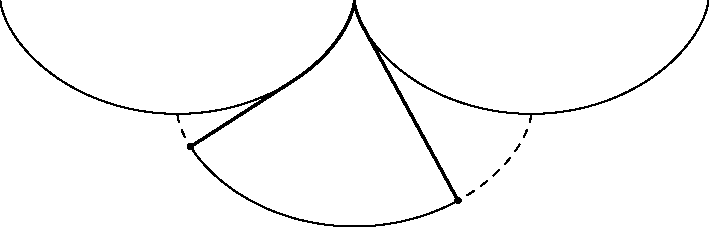
\includegraphics[width=12cm]{./img/Pendulum.pdf}
	\caption{Циклоидный маятник}
	\label{fig:Pendulum}
\end{figure}

Рассмотрим маятник, у которого нить закреплена в вершине между двумя циклоидами (рис. \ref{fig:Pendulum}). Оказывается, свободный конец нити такого маятника будет вырисовывать циклоиду. Ясно, что на самом деле он будет вырисовывать кусок эвольвенты этой циклоиды (просто по определению). Так что утверждение сводится к следующей задаче.

\begin{problem}
	Доказать, что одной из эвольвент циклоиды является конгруэнтная ей циклоида, сдвинутая таким образом, чтобы её <<острия>> перешли в вершины.
\end{problem}

\begin{solution}
	Уравнения эвольвент легко писать, если на исходной кривой введён натуральный параметр. В данном случае это не так, и перейти к натуральному параметру затруднительно. Однако можно заметить, что формулу \eqref{eq:Involute} легко модифицировать и на случай произвольного параметра:
	\[
		\widehat{\vec{r}}(t) = \vec{r}(t) - \frac{\vec{r}^\prime(t)}{\abs{\vec{r}^\prime(t)}}\int\limits_{t_0}^t\abs{\vec{r}^\prime(t)}dt.
	\]

	Действительно, мы просто везде выразили натуральный параметр $s$ через какой-то произвольный параметр $t$. Вычисляем всё, что нужно, положив $t_0 = \pi$ (так обнуляется константа в определённом интеграле).
	\begin{gather*}
		\vec{r}^\prime(t) = (1 - \cos t, -\sin t),\\
		\abs{\vec{r}^\prime(t)}^2 = (1 - \cos t)^2 + \sin^2t = 2(1 - \cos t) = 4\sin^2\frac{t}{2} \Rightarrow \abs{\vec{r}^\prime(t)} = 2\sin\frac{t}{2},\\
		\int\limits_\pi^t 2\sin\frac{t}{2}\,dt = 4\int\limits_\pi^t\sin\frac{t}{2}\,d\br{\frac{t}{2}} = -4\left.\cos\frac{t}{2}\right|_\pi^t = -4\cos\frac{t}{2}.
	\end{gather*}
	А теперь пишем, собственно, уравнение эвольвенты:
	\begin{multline*}
		\widehat{\vec{r}}(t) = (t - \sin t, \cos t - 1) - \frac{\bcancel{2}\br{\sin^{\cancel{2}}\frac{t}{2}, -\cancel{\sin\frac{t}{2}}\cos\frac{t}{2}}}{\bcancel{2} \cdot \cancel{\sin\frac{t}{2}}} \cdot \br{-4\cos\frac{t}{2}} =\\ = (t - \sin t, \cos t - 1) + 2\br{2\sin\frac{t}{2}\cos\frac{t}{2}, -2\cos^2\frac{t}{2}} =\\ = (t - \sin t, \cos t - 1) + (2\sin t, -2 - 2\cos t) = (t + \sin t, -\cos t - 3).
	\end{multline*}
	Итак, получили \[\widehat{\vec{r}}(t) = (t + \sin t, -\cos t - 3) = \big((t + \pi) - \sin(t + \pi), \cos(t + \pi) - 1\big) - (\pi, 2).\]

	Видно, что это сдвинутая циклоида. Легко проверить, что она сдвинута именно так, как указано в условии.
\end{solution}

Теперь мы можем доказать главное утверждение --- что период колебания такого маятника не зависит от амплитуды. Сформулировано оно здесь так же, как в задачнике.

\begin{problem}
	Доказать, что период колебаний материальной точки малой массы, движущейся по чаше перевёрнутой циклоиде без трения в поле силы тяжести, не зависит от её начального положения.
\end{problem}

% TODO: Дописать!


\section{Двумерные поверхности в трёхмерном пространстве}

\epigraph{Это яма, вырытая для нас великими предшественниками.}{А.\,А. Гайфуллин}

\subsection{Криволинейные системы координат в $\R^n$}

Рассмотрим область $U$ пространства $\R^n$ с декартовыми координатами $(x^1, \ldots, x^n)$. Предположим, что в другом экземпляре пространства $\R^n$ с координатами $(u^1, \ldots, u^n)$ задана область $V$ и установлено взаимно однозначное соответствие между точками областей $U$ и $V$. В этом случае для задания точки области $U$ мы можем использовать набор чисел $(u^1, \ldots, u^n)$ --- декартовы координаты соответствующей точки в области $V$.

\begin{definition}
	Будем говорить, что $(u^1, \ldots, u^n)$ являются \textit{криволинейными координатами} в области $U$, если:
	\begin{enumerate}[nolistsep, label=(\arabic*)]
		\item функции
			\[
				x^i = x^i(u^1, \ldots, u^n),
			\]
			задающие биекцию между областями $U$ и $V$, достаточно гладкие в области $V$;
		\item якобиан $\ds J = \det\br{\frac{\partial x^i}{\partial u^j}}$ отличен от нуля в области $V$ (\textit{условие регулярности});
	\end{enumerate}
\end{definition}

По теореме об обратной функции (якобиан не равен нулю) существуют достаточно гладкие обратные отображения $u^i = u^i(x^1, \ldots, x^n)$, причём якобиан $\ds\widetilde{J} = \det\br{\frac{\partial u^i}{\partial x^j}}$ отличен от нуля (он равен $J^{-1}$).

В области $U$ условия $u^i = \const$ определяют $n$ семейств \textit{координатных гиперповерхностей}. (Координатные гиперповерхности одного и того же семейства не пересекаются.)

Любые $n - 1$ координатных гиперповерхностей, принадлежащих различным семействам, пересекаются по некоторой кривой. Такие кривые называют \textit{координатными линиями}.

\begin{definition}
	Система криволинейных координат, вектора скорости координатных линий которой перпендикулярны друг другу, называется \textit{ортогональной}.
\end{definition}

\begin{problem}
	Для эллипсоидальной системы координат, определяемой равенствами
	\begin{gather*}
		x_1^2 = \frac{(a_1 - u_1)(a_1 - u_2)(a_1 - u_3)}{(a_2 - a_1)(a_3 - a_1)},\\
		x_2^2 = \frac{(a_2 - u_1)(a_2 - u_2)(a_2 - u_3)}{(a_3 - a_2)(a_1 - a_2)},\\
		x_3^2 = \frac{(a_3 - u_1)(a_3 - u_2)(a_3 - u_3)}{(a_1 - a_3)(a_2 - a_3)},
	\end{gather*}
	где $a_1 > a_2 > a_3 > 0$, $u_1 < a_3 < u_2 < a_2 < u_3 < a_1$,
	\begin{enumerate}[nolistsep, label=(\arabic*)]
		\item найти координатные поверхности и координатные линии;
		\item посчитать определители $\ds\det\br{\frac{\partial x_i}{\partial u_j}}$ и $\ds\det\br{\frac{\partial u_i}{\partial x_j}}$ и установить, в каких точках пространства $\R^3$ нарушается взаимная однозначность соответствия между криволинейными и прямоугольными декартовыми координатами;
		\item определить, является ли эта система координат ортогональной.
	\end{enumerate}
\end{problem}

\pagebreak

\begin{solution}
	\begin{enumerate}[nolistsep, label=(\arabic*)]
		\item Фиксируем $u_1 = \lambda$. Тогда
			\begin{multline*}
				\frac{x_1^2}{a_1 - \lambda} + \frac{x_2^2}{a_2 - \lambda} + \frac{x_3^2}{a_3 - \lambda} = \frac{(a_1 - u_2)(a_1 - u_3)}{(a_2 - a_1)(a_3 - a_1)} + \frac{(a_2 - u_2)(a_2 - u_3)}{(a_3 - a_2)(a_1 - a_2)} + {}\\{} + \frac{(a_3 - u_2)(a_3 - u_3)}{(a_1 - a_3)(a_2 - a_3)} = \frac{1}{(a_1 - a_2)(a_2 - a_3)(a_3 - a_1)}\Big((a_3 - a_2)(a_1 - u_2)(a_1 - u_3) + {}\\{} + (a_1 - a_3)(a_2 - u_2)(a_2 - u_3) + (a_2 - a_1)(a_3 - u_2)(a_3 - u_3)\Big) = \varphi(u_2, u_3).
			\end{multline*}

			При этом $\varphi = Au_2 + Bu_3 + Cu_2u_3 + D$. Нетрудно убедиться, что все коэффициенты, кроме $D$, нулевые, а $D$ равен $1$. Например, для коэффициента при $u_2$ имеем
			\begin{multline*}
				(\ldots) \cdot A = (a_1a_2 - a_1a_3) + (a_2a_3 - a_1a_2) + (a_1a_3 - a_2a_3) = \\= \cancel{(a_1a_2 - a_1a_2)} + \cancel{(a_2a_3 - a_2a_3)} + \cancel{(a_3a_1 - a_3a_1)} = 0.
			\end{multline*}

			Отсюда, $\varphi \equiv 1$. Итак, имеем координатные поверхности
			\[
				\frac{x_1^2}{a_1 - \lambda} + \frac{x_2^2}{a_2 - \lambda} + \frac{x_3^2}{a_3 - \lambda} = 1,
			\]
			представляющие собой эллипсоиды.

			Для остальных координат всё аналогично. Фиксируя $u_2 = \mu$, получаем семейство однополостных гиперболоидов:
			\[
				\frac{x_1^2}{a_1 - \mu} + \frac{x_2^2}{a_2 - \mu} - \frac{x_3^2}{\mu - a_3} = 1.
			\]
			(Формула та же, но $a_3 < \mu$.) Для фиксированного $u_3 = \nu$ получаем семейство двуполостных гиперболоидов:
			\[
				\frac{x_1^2}{a_1 - \nu} - \frac{x_2^2}{\nu - a_2} - \frac{x_3^2}{\nu - a_3} = 1.
			\]
		\item Найдём, например, производную $\partial x_1 / \partial u_2$:
			\begin{gather*}
				x_1(u_2) = \sqrt{\frac{(a_1 - u_1)(a_1 - u_2)(a_1 - u_3)}{(a_2 - a_1)(a_3 - a_1)}} = \sqrt{\frac{(a_1 - u_1)(a_1 - u_3)}{(a_2 - a_1)(a_3 - a_1)}} \cdot \sqrt{a_1 - u_2},\\
				\frac{\partial x_1}{\partial u_2} = \sqrt{\frac{(a_1 - u_1)(a_1 - u_3)}{(a_2 - a_1)(a_3 - a_1)}} \cdot \frac{-1}{2\sqrt{a_1 - u_2}} = -\frac{1}{2}\sqrt{\frac{(a_1 - u_1)(a_1 - u_3)}{(a_2 - a_1)(a_3 - a_1)(a_1 - u_2)}}.
			\end{gather*}
			Отсюда понятен общий вид выражения $\partial x_i / \partial u_j$. Считаем определитель:
			\begin{fullwidth}
				\begin{multline*}
					\det\br{\frac{\partial x_i}{\partial u_j}} =\\ = -\frac{1}{8}\det
					\begin{pmatrix}
						\sqrt{\frac{(a_1 - u_2)(a_1 - u_3)}{(a_2 - a_1)(a_3 - a_1)(a_1 - u_1)}} & \sqrt{\frac{(a_1 - u_1)(a_1 - u_3)}{(a_2 - a_1)(a_3 - a_1)(a_1 - u_2)}} & \sqrt{\frac{(a_1 - u_1)(a_1 - u_2)}{(a_2 - a_1)(a_3 - a_1)(a_1 - u_3)}}\\
						\sqrt{\frac{(a_2 - u_2)(a_2 - u_3)}{(a_1 - a_2)(a_3 - a_2)(a_2 - u_1)}} & \sqrt{\frac{(a_2 - u_1)(a_2 - u_3)}{(a_1 - a_2)(a_3 - a_2)(a_2 - u_2)}} & \sqrt{\frac{(a_2 - u_1)(a_2 - u_2)}{(a_1 - a_2)(a_3 - a_2)(a_2 - u_3)}}\\
						\sqrt{\frac{(a_3 - u_2)(a_3 - u_3)}{(a_1 - a_3)(a_2 - a_3)(a_3 - u_1)}} & \sqrt{\frac{(a_3 - u_1)(a_3 - u_3)}{(a_1 - a_3)(a_2 - a_3)(a_3 - u_2)}} & \sqrt{\frac{(a_3 - u_1)(a_3 - u_2)}{(a_1 - a_3)(a_2 - a_3)(a_3 - u_3)}}
					\end{pmatrix} =\\ =
					\frac{1}{8} \cdot \frac{1}{(a_1 - a_2)(a_2 - a_3)(a_3 - a_1)}\det
					\begin{pmatrix}
						\sqrt{\frac{(a_1 - u_2)(a_1 - u_3)}{a_1 - u_1}} & \sqrt{\frac{(a_1 - u_1)(a_1 - u_3)}{a_1 - u_2}} & \sqrt{\frac{(a_1 - u_1)(a_1 - u_2)}{a_1 - u_3}}\\
						\sqrt{\frac{(a_2 - u_2)(a_2 - u_3)}{a_2 - u_1}} & \sqrt{\frac{(a_2 - u_1)(a_2 - u_3)}{a_2 - u_2}} & \sqrt{\frac{(a_2 - u_1)(a_2 - u_2)}{a_2 - u_3}}\\
						\sqrt{\frac{(a_3 - u_2)(a_3 - u_3)}{a_3 - u_1}} & \sqrt{\frac{(a_3 - u_1)(a_3 - u_3)}{a_3 - u_2}} & \sqrt{\frac{(a_3 - u_1)(a_3 - u_2)}{a_3 - u_3}}
					\end{pmatrix} =\\ = \frac{1}{8} \cdot \frac{1}{(a_1 - a_2)(a_2 - a_3)(a_3 - a_1)} \sqrt{-\prod_{i, j = 1}^3(a_i - u_j)} \cdot \det
					\begin{pmatrix}
						\frac{1}{a_1 - u_1} & \frac{1}{a_1 - u_2} & \frac{1}{a_1 - u_3}\\
						\frac{1}{a_2 - u_1} & \frac{1}{a_2 - u_2} & \frac{1}{a_2 - u_3}\\
						\frac{1}{a_3 - u_1} & \frac{1}{a_3 - u_2} & \frac{1}{a_3 - u_3}
					\end{pmatrix}.
				\end{multline*}
			\end{fullwidth}
			 Чтобы вычислить оставшийся определитель, вычтем первую строку из двух других:
			\begin{multline*}
				\det
				\begin{pmatrix}
					\frac{1}{a_1 - u_1} & \frac{1}{a_1 - u_2} & \frac{1}{a_1 - u_3}\\
					\frac{1}{a_2 - u_1} & \frac{1}{a_2 - u_2} & \frac{1}{a_2 - u_3}\\
					\frac{1}{a_3 - u_1} & \frac{1}{a_3 - u_2} & \frac{1}{a_3 - u_3}
				\end{pmatrix} = \det
				\begin{pmatrix}
					\frac{1}{a_1 - u_1} & \frac{1}{a_1 - u_2} & \frac{1}{a_1 - u_3}\\
					\frac{a_1 - a_2}{(a_1 - u_1)(a_2 - u_1)} & \frac{a_1 - a_2}{(a_1 - u_2)(a_2 - u_2)} & \frac{a_1 - a_2}{(a_1 - u_3)(a_2 - u_3)}\\
					\frac{a_1 - a_3}{(a_1 - u_1)(a_3 - u_1)} & \frac{a_1 - a_3}{(a_1 - u_2)(a_3 - u_2)} & \frac{a_1 - a_3}{(a_1 - u_3)(a_3 - u_3)}\\
				\end{pmatrix} = \\ = (a_1 - a_2)(a_1 - a_3) \cdot \det
				\begin{pmatrix}
					\frac{1}{a_1 - u_1} & \frac{1}{a_1 - u_2} & \frac{1}{a_1 - u_3}\\
					\frac{1}{(a_1 - u_1)(a_2 - u_1)} & \frac{1}{(a_1 - u_2)(a_2 - u_2)} & \frac{1}{(a_1 - u_3)(a_2 - u_3)}\\
					\frac{1}{(a_1 - u_1)(a_3 - u_1)} & \frac{1}{(a_1 - u_2)(a_3 - u_2)} & \frac{1}{(a_1 - u_3)(a_3 - u_3)}
				\end{pmatrix} =\\ =
				\frac{(a_1 - a_2)(a_1 - a_3)}{(a_1 - u_1)(a_1 - u_2)(a_1 - u_3)}\det
				\begin{pmatrix}
					1 & 1 & 1\\
					\frac{1}{a_2 - u_1} & \frac{1}{a_2 - u_2} & \frac{1}{a_2 - u_3}\\
					\frac{1}{a_3 - u_1} & \frac{1}{a_3 - u_2} & \frac{1}{a_3 - u_3}
				\end{pmatrix}.
			\end{multline*}
			Здесь вычтем первый столбец из двух остальных:
			\begin{multline*}
				\det\begin{pmatrix}
					1 & 1 & 1\\
					\frac{1}{a_2 - u_1} & \frac{1}{a_2 - u_2} & \frac{1}{a_2 - u_3}\\
					\frac{1}{a_3 - u_1} & \frac{1}{a_3 - u_2} & \frac{1}{a_3 - u_3}
				\end{pmatrix} = \det
				\begin{pmatrix}
					1 & 0 & 0\\
					\frac{1}{a_2 - u_1} & \frac{u_1 - u_2}{(a_2 - u_2)(a_2 - u_1)} & \frac{u_1 - u_3}{(a_2 - u_1)(a_2 - u_3)}\\
					\frac{1}{a_3 - u_1} & \frac{u_1 - u_2}{(a_3 - u_2)(a_3 - u_1)} & \frac{u_1 - u_3}{(a_3 - u_1)(a_3 - u_3)}
				\end{pmatrix} =\\ = \det
				\begin{pmatrix}
					\frac{u_1 - u_2}{(a_2 - u_2)(a_2 - u_1)} & \frac{u_1 - u_3}{(a_2 - u_1)(a_2 - u_3)}\\
					\frac{u_1 - u_2}{(a_3 - u_2)(a_3 - u_1)} & \frac{u_1 - u_3}{(a_3 - u_1)(a_3 - u_3)}
				\end{pmatrix} = \frac{(u_1 - u_2)(u_1 - u_3)}{(a_2 - u_1)(a_3 - u_1)}\det
				\begin{pmatrix}
					\frac{1}{a_2 - u_2} & \frac{1}{a_2 - u_3}\\
					\frac{1}{a_3 - u_2} & \frac{1}{a_3 - u_3}
				\end{pmatrix} =\\ =
				\frac{(u_1 - u_2)(u_1 - u_3)}{(a_2 - u_1)(a_3 - u_1)}\br{\frac{1}{(a_2 - u_2)(a_3 - u_3)} - \frac{1}{(a_3 - u_2)(a_2 - u_3)}} =\\ = \frac{(u_1 - u_2)(u_1 - u_3)(u_2 - u_3)(a_3 - a_2)}{(a_2 - u_1)(a_3 - u_1)(a_2 - u_2)(a_3 - u_3)(a_3 - u_2)(a_2 - u_3)}.
			\end{multline*}

			Подставляем результат в промежуточную формулу:
			\[
				\frac{(a_1 - a_2)(a_2 - a_3)(a_3 - a_1)}{-\prod\limits_{i, j = 1}^3(a_i - u_j)}(u_1 - u_2)(u_2 - u_3)(u_3 - u_1).
			\]
			И, наконец, пишем ответ:
			\[
				\det\br{\frac{\partial x_i}{\partial u_j}} =
				\frac{(u_1 - u_2)(u_2 - u_3)(u_3 - u_1)}{8\sqrt{-\prod\limits_{i, j = 1}^3(a_i - u_j)}}.
			\]

			Взаимная однозначность координат нарушается в точках, где якобиан равен $0$. Как видно из выведенной нами формулы, это происходит при $u_i = u_j$ (для каких-то $i \ne j$). Однако по условию $u_1 < u_2 < u_3$, так что в выбранной области эллипсоидальные координаты взаимно однозначны.
		\item Из полученных уравнений координатных поверхностей видно, что они образуют квадрики, являющиеся телами вращения софокусных эллипсов и гипербол. А как известно из курса аналитической геометрии, софокусные эллипс и гипербола перпендикулярны друг другу. (А софокусные друг другу эллипсы не пересекаются, как и софокусные друг другу гиперболы.) Значит, и координатные линии, получающиеся как пересечения таких координатных поверхностей, перпендикулярны друг другу. Так что данная система координат является ортогональной.
	\end{enumerate}
\end{solution}

\begin{problem}
	Преобразовать \textit{оператор Лапласа} $\Delta V \vcentcolon = \ds\frac{\partial^2V}{\partial x^2} + \frac{\partial^2V}{\partial y^2}$ к полярным координатам $x = \rho\cos\varphi$, $y = \rho\sin\varphi$.
\end{problem}

\begin{solution}
	Формулы перехода от декартовых координат к полярным имеют вид
	\[
		\rho = \sqrt{x^2 + y^2},\quad \tg\varphi = \frac{y}{x}.
	\]
	Выражаем частные производные первого порядка:
	\[
		\frac{\partial V}{\partial x} = \frac{\partial V}{\partial \rho}\frac{\partial\rho}{\partial x} + \frac{\partial V}{\partial \varphi}\frac{\partial \varphi}{\partial x}.
	\]
	Здесь $V^\prime_\rho$ и $V^\prime_\varphi$ --- то, что нам нужно. Осталось выразить частные производные $\rho^\prime_x$ и $\varphi^\prime_x$.
	\[
		\frac{\partial\rho}{\partial x} = (\sqrt{x^2 + y^2})^\prime_x = \frac{x}{\sqrt{x^2 + y^2}} = \frac{\cancel{r}\cos\varphi}{\cancel{r}} = \cos\varphi.
	\]

	Отметим, что для вычисления $\varphi^\prime_x$ нельзя просто взять $\arctg$ от обеих частей выражения $\tg\varphi = y / x$, ведь $\varphi$ меняется от $0$ до $2\pi$, а областью значений функции $\arctg$ является интервал $\br{-\frac{\pi}{2}; \frac{\pi}{2}}$. Вместо этого выражение можно продифференцировать (по $x$):
	\[\begin{tikzcd}
		{\displaystyle\frac{1}{\cos^2\varphi}\frac{\partial\varphi}{\partial x}} & {\displaystyle\frac{\partial}{\partial x}(\tg\varphi)} & {\displaystyle\frac{\partial}{\partial x}\left(\frac{y}{x}\right) = -\frac{y}{x^2}}.
		\arrow[equals, from=1-2, to=1-1]
		\arrow[equals, from=1-2, to=1-3]
	\end{tikzcd}\]
	Отсюда находим $\displaystyle\frac{\partial\varphi}{\partial x} = -\frac{y}{x^2}\cos^2\varphi = -\frac{\sin\varphi}{\rho}$. Итого,
	\[
		\frac{\partial V}{\partial x} = \frac{\partial V}{\partial \rho}\cos\varphi - \frac{\partial V}{\partial \varphi} \frac{\sin\varphi}{\rho}.
	\]
	Аналогично находим
	\[
		\frac{\partial V}{\partial y} = \frac{\partial V}{\partial\rho}\frac{\cos\varphi}{\rho} + \frac{\partial V}{\partial \varphi}\sin\varphi.
	\]
	Переходим к нахождению вторых производных.
	\begin{multline*}
		\frac{\partial^2V}{\partial x^2} = \frac{\partial}{\partial x}\br{\frac{\partial V}{\partial x}} = \frac{\partial}{\partial\rho}\br{\frac{\partial V}{\partial x}} \cdot \frac{\partial\rho}{\partial x} + \frac{\partial}{\partial\varphi}\br{\frac{\partial V}{\partial x}} \cdot \frac{\partial\varphi}{\partial x} =\\ = \br{\frac{\partial^2V}{\partial\rho^2}\cos\varphi - \frac{\partial^2V}{\partial\varphi\partial\rho}\frac{\sin\varphi}{\rho} + \frac{\partial V}{\partial\varphi}\frac{\sin\varphi}{\rho^2}} \cdot \cos\varphi + {}\\{} + \br{\frac{\partial^2 V}{\partial\rho\partial\varphi}\cos\varphi - \frac{\partial V}{\partial\rho}\sin\varphi - \frac{\partial^2V}{\partial\varphi^2}\frac{\sin\varphi}{\rho} - \frac{\partial V}{\partial\varphi}\frac{\cos\varphi}{\rho}} \cdot \br{-\frac{\sin\varphi}{\rho}}.
	\end{multline*}
	Раскрывая скобки, получаем
	\[
		\frac{\partial^2V}{\partial x^2} = \frac{\partial^2V}{\partial\rho^2}\cos^2\varphi - \frac{\partial^2V}{\partial\rho\partial\varphi}\frac{\sin 2\varphi}{\rho} + \frac{\partial^2V}{\partial\varphi^2}\frac{\sin^2\varphi}{\rho^2} + \frac{\partial V}{\partial\varphi}\frac{\sin 2\varphi}{\rho^2} + \frac{\partial V}{\partial\rho}\frac{\sin^2\varphi}{\rho}.
	\]
	Аналогично находим
	\[
		\frac{\partial^2V}{\partial y^2} = \frac{\partial^2 V}{\partial\rho^2}\sin^2\varphi + \frac{\partial^2V}{\partial\rho\partial\varphi}\frac{\sin 2\varphi}{\rho} + \frac{\partial^2V}{\partial\varphi^2}\frac{\cos^2\varphi}{\rho^2} + \frac{\partial V}{\partial\rho}\frac{\cos^2\varphi}{\rho} - \frac{\partial V}{\partial\varphi}\frac{\sin 2\varphi}{\rho^2}.
	\]
	Полученные выражения нужно сложить:
	\begin{multline*}
		\Delta V = \frac{\partial V}{\partial x^2} + \frac{\partial V}{\partial y^2} = \frac{\partial^2 V}{\partial\rho^2}\underbrace{(\cos^2\varphi + \sin^2\varphi)}_{1} + \frac{\partial^2V}{\partial\varphi^2}\underbrace{\br{\frac{\sin^2\varphi + \cos^2\varphi}{\rho^2}}}_{1 / \rho^2} + {}\\{} + \frac{\partial V}{\partial\rho\partial\varphi}\underbrace{\br{-\frac{\sin 2\varphi}{\rho} + \frac{\sin 2\varphi}{\rho}}}_{0} + \frac{\partial V}{\partial\rho}\underbrace{\br{\frac{\sin^2\varphi + \cos^2\varphi}{\rho}}}_{1 / \rho} + \frac{\partial V}{\partial\varphi}\underbrace{\br{-2\frac{\sin 2\varphi}{\rho^2} + 2\frac{\sin 2\varphi}{\rho^2}}}_{0}.
	\end{multline*}

	\noindent
	Получаем итоговое выражение оператора Лапласа в полярных координатах:
	\[
		\Delta V = \frac{\partial^2V}{\partial\rho^2} + \frac{1}{\rho^2}\frac{\partial^2V}{\partial\varphi^2} + \frac{1}{\rho}\frac{\partial V}{\partial\rho}.
	\]
	Эту формулу часто записывают в виде
	\[
		\Delta V = \frac{1}{\rho}\frac{\partial}{\partial\rho}\br{\rho\frac{\partial V}{\partial{\rho}}} + \frac{1}{\rho^2}\frac{\partial^2V}{\partial\varphi^2}.
	\]
\end{solution}

\vspace{-.3cm}\subsection{Риманова метрика в криволинейных координатах}

Функции $x^i = x^i(u^1, \ldots, u^n)$ удобно рассматривать одновременно для всех $i = 1, \ldots, n$, используя для этого вектор-функцию
\[
	\vec{r} = \vec{r}(u^1, \ldots, u^n),\text{ где $\vec{r} = (x^1, \ldots, x^n)$}.
\]

Векторы $\vec{r}_i \vcentcolon = \partial \vec{r} / \partial u^i$ имеют направления касательных к координатным линиям, так что в каждой точке области $U$ они линейно независимы. Они определяют в окрестности некоторой точки $(u^1, \ldots, u^n)$ малый вектор $\d\vec{r} = \vec{r}_i\d u^i$. Квадрат его длины, выраженный в криволинейных координатах, определяет метрику:
\[
	\d s^2 = \langle \d\vec{r}, \d\vec{r}\rangle = \left\langle\vec{r}_i\d u^i, \vec{r}_j\d u^j\right\rangle = g_{ij}\d u^i\d u^j,
\]
где $g_{ij} = \langle\vec{r}_i, \vec{r}_j\rangle$ --- элементы матрицы Грама векторов $\vec{r}_1, \ldots, \vec{r}_n$. При переходе к другим координатам $\widetilde{u}^1, \ldots, \widetilde{u}^n$ матрица Грама преобразуется так, как и положено преобразовываться матрице квадратичной формы (по тензорному закону):
\begin{equation} \label{eq:RiemannCoordinates}
	\widetilde{g}_{ij} = \left\langle\frac{\partial \vec{r}}{\partial\widetilde{u}^i}, \frac{\partial \vec{r}}{\partial\widetilde{u}^j}\right\rangle = \left\langle\frac{\partial \vec{r}}{\partial u^k}\frac{\partial u^k}{\partial\widetilde{u}^i}, \frac{\partial \vec{r}}{\partial u^l}\frac{\partial u^l}{\partial\widetilde{u}^j}\right\rangle = \frac{\partial u^k}{\partial\widetilde{u}^i}\frac{\partial u^l}{\partial\widetilde{u}^j}g_{kl}.
\end{equation}

\begin{definition} \label{definition:RiemannMetrics}
	Говорят, что в области $U \subset \R^n$ задана \textit{риманова метрика}, если для любой криволинейной системы координат $(u^1, \ldots, u^n)$ в $U$ задана матрица $g_{ij}(u)$, которая:
	\begin{enumerate}[nolistsep, label=(\arabic*)]
		\item симметрична: $g_{ij}(u) = g_{ji}(u)$;
		\item невырожденна и положительно определена;
		\item при замене координат изменяется по формулам \eqref{eq:RiemannCoordinates}.
	\end{enumerate}
\end{definition}

\begin{problem} \label{problem:CylindricalMetric}
	Записать евклидову метрику в цилиндрической системе координат.
\end{problem}

\begin{solution}
	Запишем дифференциалы евклидовых координат:
	\begin{gather*}
		\d x = \d(\rho\cos\varphi) = \cos\varphi\d\rho - \rho\sin\varphi\d\varphi,\\
		\d y = \d(\rho\sin\varphi) = \sin\varphi\d\rho + \rho\cos\varphi\d\varphi,\\
		\d z = \d h.
	\end{gather*}
	Подставляем их в запись евклидовой метрики:
	\begin{multline*}
		\d s^2 = \d x^2 + \d y^2 + \d z^2 = (\cos\varphi\d\rho - \rho\sin\varphi\d\varphi)^2 + (\sin\varphi\d\rho + \rho\cos\varphi\d\varphi)^2 + \d h^2 =\\ = \underbrace{(\cos^2\varphi + \sin^2\varphi)}_{= 1}\d\rho^2 - \cancel{\rho\sin(2\varphi)\d\rho\d\varphi} + \rho^2\underbrace{(\cos^2\varphi + \sin^2\varphi)}_{= 1}\d\varphi^2 + {}\\{} + \cancel{\rho\sin(2\varphi)\d\rho\d\varphi} + \d h^2 = \d\rho^2 + \rho^2\d\varphi^2 + \d h^2.
	\end{multline*}
\end{solution}

Пусть имеем параметризованную кривую $\vec{r}(t)$ в криволинейных координатах $(u^1, \ldots, u^n)$ с римановой метрикой, заданной матрицей $G = g_{ij}$. Измеряем длину кривой, заметаемой при изменении параметра от $a$ до $b$:
\begin{equation} \label{eq:RiemannLength}
	\ell = \int\limits_a^b\abs{\frac{\d\vec{r}}{\d t}}\d t = \int\limits_a^b\sqrt{\left\langle \frac{\d\vec{r}}{\d t}, \frac{\d\vec{r}}{\d t} \right\rangle}\d t = \int\limits_a^b\sqrt{\frac{\d s^2}{(\d t)^2}}\d t = \int\limits_a^b\sqrt{g_{ij}\frac{\d u^i}{\d t}\frac{\d u^j}{\d t}}\d t.
\end{equation}

\begin{problem}
	Проверить, что матрица
	\[
		\G(u, v) = \frac{1}{1 - u^2 - v^2}
		\begin{pmatrix}
			1 - v^2 & uv\\
			uv & 1 - u^2
		\end{pmatrix}
	\]
	задаёт риманову метрику в единичном круге на плоскости с координатами $(u, v)$. Вычислить в этой метрике длину кривой $u^2 + v^2 = a^2$, где $0 < a < 1$.
\end{problem}

\begin{proof}
	Нужно проверить лишь то, что матрица $G$ невырожденна и положительно определена, для этого можно воспользоваться критерием Сильвестра. Для минора $1 \times 1$ всё очевидно, остаётся проверить знак определителя всей матрицы $2 \times 2$:
	\[
		\det\G = \frac{(1 - v^2)(1 - u^2) - u^2v^2}{1 - u^2 - v^2} = \frac{\cancel{1 - u^2 - v^2}}{\cancel{1 - u^2 - v^2}} = 1.
	\]
	
	Если параметризовать нашу кривую как $\vec{r}(t) = (u(t), v(t))$, где $u(t) = a\cos t$, $v(t) = a\sin t$ (где $t$ меняется от $0$ до $2\pi$), то длина вычисляется по формуле \eqref{eq:RiemannLength}:
	\[
		\ell = \int\limits_0^{2\pi}\sqrt{\begin{pmatrix}\dot{u}(t) & \dot{v}(t)\end{pmatrix} \G \begin{pmatrix}\dot{u}(t) \\ \dot{v}(t) \end{pmatrix}}\d t.
	\]
	Подставляем:
	\begin{multline*}
		\int\limits_0^{2\pi}\sqrt{\begin{pmatrix}-a\sin t & a\cos t\end{pmatrix} \cdot \left(\frac{1}{1 - a^2}\begin{pmatrix} 1 - a^2\sin^2t & a^2\sin t\cos t \\ a^2\sin t\cos t & 1 - a^2\cos^2t \end{pmatrix}\right) \cdot \begin{pmatrix} -a\sin t \\ a\cos t \end{pmatrix}}\d t =\\ = \int\limits_0^{2\pi}\sqrt{\begin{pmatrix} -a\sin t & a\cos t \end{pmatrix} \cdot \left(\frac{1}{\cancel{1 - a^2}}\begin{pmatrix} -a\sin t\cancel{(1 - a^2)} \\ a\cos t\cancel{(1 - a^2)}\end{pmatrix}\right)}\d t =\\ = \int\limits_0^{2\pi}\sqrt{a^2(\cos^2t + \sin^2t)}\d t = \int\limits_0^{2\pi}a\d t = 2\pi a.
	\end{multline*}
\end{proof}

Правильно думать, что матрица $\G(u^1, \ldots, u^n)$ (как матрица Грама линейно независимых векторов) симметрична и положительно определена, а потому задаёт скалярное произведение (своё в каждой точке области $U \subset \R^n$). В криволинейной системе координат $(u^1, \ldots, u^n)$ мы работаем именно в этом скалярном произведении. Например, можем считать длины кривых (что уже было продемонстрировано) или углы между кривыми.

\begin{problem}
	Найти угол между кривыми $v = 2u + 1$ и $v = -2u + 1$ на плоскости с координатами $(u, v)$ с метрикой
	\[
		\d s^2 = 2\d u^2 + 2\d u\d v + 4\d v^2.
	\]
\end{problem}

\begin{solution}
	Данная в условии метрика задаётся матрицей
	\[
		\G =
		\begin{pmatrix}
			2 & 1\\
			1 & 4
		\end{pmatrix}.
	\]

	Параметризуем обе эти кривые: $\vec{r}_1(t) = (t, 2t + 1)$, $\vec{r}_2(t) = (t, -2t + 1)$. Они пересекаются в единственной точке $(0, 1)$ при $t = 0$. Вектора скорости этих кривых в данной точке есть $\vec{v}_1 = (1, 2)$, $\vec{v}_2 = (1, -2)$. Находим угол между этими векторами по формуле:
	\[
		\cos\angle(\vec{v}_1, \vec{v}_2) = \frac{\langle\vec{v}_1, \vec{v}_2\rangle_\G}{\sqrt{\langle\vec{v}_1, \vec{v}_1\rangle_\G} \cdot \sqrt{\langle\vec{v}_2, \vec{v}_2\rangle_\G}} = \frac{-14}{\sqrt{22} \cdot \sqrt{14}} = -\sqrt{\frac{7}{11}}.
	\]
	Отсюда получаем $\angle(\vec{v}_1, \vec{v}_2) = \arccos\sqrt{\frac{7}{11}}$.
\end{solution}

\subsection{Определение поверхности. Локальные координаты}

Наиболее наглядными и интересными с геометрической точки зрения для нас будут двумерные поверхности в $\R^3$, поэтому повествование будет строиться именно вокруг них.

%\begin{definition}
%	Множество точек $\M \subset \R^3$ образует \textit{регулярную поверхность}, если в достаточно малой окрестности $U \subset \R^3$ каждой своей точки множество $\M$ задаётся как образ гладкого отображения
%	\[
%		\vec{r}\colon (u, v) \mapsto \big(x(u, v), y(u, v), z(u, v)\big)
%	\]
%	из области $V \subset \R^2$ в $U$, и в каждой точке из $V$ векторы $\vec{r}_u = \partial\vec{r} / \partial u$ и $\vec{r}_v = \partial\vec{r} / {\partial v}$ линейно независимы (\textit{условие регулярности}).
%\end{definition}
%
%Поверхности можно задавать не только параметрически, но и как множество нулей гладкой функции или в виде графика. Обсудим локальную эквивалентность таких заданий.
%
%\begin{proposition} \label{proposition:SurfaceGraph}
%	Множество точек $\M \subset \R^3$ образует регулярную поверхность тогда и только тогда, когда в окрестности каждой своей точки оно представляется как график гладкой функции $z = f(x, y)$ в подходящих декартовых координатах $x$, $y$, $z$.
%\end{proposition}
%
%\begin{proof}
%	График функции является частным случаем параметрического задания, поэтому достаточно доказать только часть <<тогда>>. Пусть $(u_0, v_0) \in V$. Векторы $\vec{r}_u$ и $\vec{r}_v$ линейно независимы всюду, так что без ограничения общности можно считать, что минор
%	$
%		\begin{pmatrix}
%			x_u & x_v\\
%			y_u & y_v
%		\end{pmatrix}
%	$
%	обратим в точке $(u_0, v_0)$. По теореме об обратной функции в некоторой окрестности точки $(x(u_0, v_0), y(u_0, v_0))$ определено обратное отображение
%	\[
%		(x, y) \mapsto \big(u(x, y), v(x, y)\big).
%	\]
%
%	Поэтому в достаточно малой окрестности точки $\vec{r}(u_0, v_0)$ поверхность задаётся как график функции $z = z(u(x, y), v(x, y)) = z(x, y)$.
%\end{proof}
%

%
%

%
%Перейдём к определению Ивана Алексеевича.

\begin{definition}
	\textit{Простым куском поверхности} в $\R^3$ называется подмножество в $\R^3$, гомеоморфное единичному кругу.
\end{definition}

\begin{definition}
	Если $\M$ --- простой кусок поверхности, то любой гомеоморфизм $\vec{r}\colon \Omega \to \M$, где $\Omega$ --- некоторая простая плоская область, называется \textit{параметризацией} куска $\M$. Параметризация называется \textit{гладкой}, если таково отображение $\vec{r}$. Она называется \textit{регулярной}, если область $\Omega$ имеет кусочно-гладкую границу и ранг матрицы дифференциала отображения $\vec{r}$ равен двум во всех точках области $\Omega$.
\end{definition}

\begin{definition}
	Простой кусок поверхности называется \textit{гладким}, если он допускает регулярную параметризацию.

	\textit{Гладкой поверхностью} в $\R^3$ будем называть любое подмножество $\M \subset \R^3$ такое, что для любой точки $\vec{x} \in \R^3$ пересечение $\M \cap \overline{B}_\eps(\vec{x})$ множества $\M$ с некоторым замкнутым шаром с центром в точке $\vec{x}$ либо пусто, либо является гладким простым куском поверхности.

	Любой гладкий простой кусок поверхности, содержащийся в $\M$, будем называть \textit{куском} поверхности $\M$.
\end{definition}

\begin{definition}
	Точка $\vec{x}$ простого куска поверхности $\M$ называется для него \textit{внутренней}, если она соответствует внутренней точке области $\Omega$ при некоторой параметризации $\Omega \to \M$. В противном случае она называется \textit{граничной}.
\end{definition}

\begin{proposition}
	Данное выше определение внутренней точки простого куска поверхности корректно, то есть не зависит от параметризации.
\end{proposition}

\begin{proof}
	Пусть $\vec{r}_1\colon \Omega_1 \to \M$ и $\vec{r}_2\colon \Omega_2 \to \M$ --- две параметризации простого куска поверхности $\M$, точка $\vec{x} \in \M$ соответствует некоторой внутренней точке области $\Omega_1$. Так как отображение $\vec{r}_1$ является гомеоморфизмом, то у точки $\vec{x}$ есть окрестность, гомеоморфная открытому диску. Но тогда и у прообраза точки $\vec{x}$ при гомеоморфизме $\vec{r}_2$ тоже есть окрестность, гомеоморфная открытому диску.
\end{proof}

\begin{definition}
	Точка $\vec{x}$ гладкой поверхности $\M$ называется для этой поверхности \textit{внутренней}, если для некоторого шара $\overline{B}_\eps(\vec{x})$ она является внутренней точкой простого куска $\M \cap \overline{B}_\eps(\vec{x})$. В противном случае она называется \textit{граничной}. Множество все граничных точек поверхности называется её \textit{краем} и обозначается через $\partial\M$.
\end{definition}

\begin{proposition}
	Край поверхности либо пуст, либо состоит из не более чем счётного числа жордановых кривых. (Замкнутой или незамкнутой \textit{жордановой кривой} называется образ вложения окружности или отрезка, соответственно.)
\end{proposition}

\begin{proof}
	Сразу следует из определения гомеоморфизма.
\end{proof}

Достаточно малая окрестность каждой точки поверхности является простым куском, на котором посредством параметризации появляется криволинейная система координат. Мы будем называть такие координаты \textit{локальными координатами} на этом простом куске. Если в некоторой области заданы две локальные системы координат, то функции, выражающие одни через другие, мы будем называть \textit{функциями перехода}.

\begin{proposition} \label{proposition:SurfaceGraph}
	В окрестности внутренней точки $\vec{x}_0$ гладкая поверхность в $\R^3$ может быть задана (без ограничения общности) уравнением вида
	\[
		z = f(x, y),
	\]
	где $f$ --- некоторая гладкая функция. В этой окрестности любые другие локальные координаты выражаются через $(x, y)$ гладкими функциями.
\end{proposition}

\begin{proof}
	Пусть $(u, v)$ --- локальные координаты в окрестности точки $\vec{x}_0$, соответствующие некоторой регуляной параметризации $\vec{r}$. Тогда матрица
	\[
		\begin{pmatrix}
			\cfrac{\partial r^1}{\partial u} & \cfrac{\partial r^2}{\partial u} & \cfrac{\partial r^3}{\partial u}\\[1em]
			\cfrac{\partial r^1}{\partial v} & \cfrac{\partial r^2}{\partial v} & \cfrac{\partial r^3}{\partial v}
		\end{pmatrix}
	\]
	имеет ранг $2$. Без ограничения общности можем считать, что невырожден минор $2 \times 2$ слева. По теореме об обратной функции координаты $u$, $v$ в окрестности точки $\vec{x}_0$ можно выразить на данной поверхности через $x$, $y$ гладкими функциями: $u = u(x, y)$, $v = v(x, y)$. Получим, что в этой окрестности поверхность задаётся уравнением $z = r^3(u(x, y), v(x, y))$.
\end{proof}

\begin{lemma} \label{lemma:SmoothLocal}
	В достаточно малых окрестностях всегда можно выбрать гладкие функции перехода между любыми локальными координатами.
\end{lemma}

\begin{proof}
	В доказательстве предложения \ref{proposition:SurfaceGraph} упоминалось, что для любых локальных координат $u$ и $v$ в некоторой области на поверхности можно построить, не ограничивая общности, гладкие функции $u = u(x, y)$, $v = v(x, y)$. Пусть в области заданы две локальные системы координат --- $(u, v)$ и $(\widetilde{u}, \widetilde{v})$. В, возможно меньшей, области можно выразить координаты $u$ и $v$ гладко через $x$ и $y$, а последние --- гладко через $\widetilde{u}$ и $\widetilde{v}$.
\end{proof}

\begin{corollary} \label{corollary:CurveOnSurface}
	Пусть $I \subset \R$ --- промежуток, отображение $\vec{\rho}\colon I \to \R^3$ задаёт кривую в $\R^3$, причём $\Im\vec{\rho} \subset \M$, где $\M$ --- гладкая поверхность в $\R^3$. Тогда для любой точки $\vec{x}_0 \in I$ и любой регулярной параметризации $\vec{r}(u, v)$ поверхности $\M$ в окрестности точки $\vec{\rho}(\vec{x}_0)$ найдутся гладкие функции $\varphi, \psi\colon I \to \R$ такие, что в этой окрестности точки $\vec{x}_0$ следующая диаграмма коммутативна:

	\shorthandoff{"}%
	\[\begin{tikzcd}
			{I \subset \R} \\
			&& {\mathcal{M} \subset\R^3} \\
			{\Omega \subset \R^2}
			\arrow["\vec{\rho}", from=1-1, to=2-3]
			\arrow["{\varphi \times \psi}"', from=1-1, to=3-1]
			\arrow["{\boldsymbol{r}}"', from=3-1, to=2-3]
	\end{tikzcd}\]
	\shorthandoff{"}%
\end{corollary}

\begin{proof}
	Поскольку любая пара локальных координат выражается через любую другую гладкими функциями, справедливость утверждения достаточно установить для какой-либо одной параметризации. Но для параметризации, заданной парой (каких-то) евклидовых координат, утверждение очевидно.
\end{proof}

Это значит, что любая кривая на поверхности может быть в окрестности каждой своей точки запараметризована в локальных координатах: $\vec{\rho}(t) = (u(t), v(t))$.

\begin{proposition}
	Множество точек $\M \subset \R^3$ образует регулярную поверхность тогда и только тогда, когда для каждой точки $\vec{x} \in \M$ существует такая окрестность $U \subset \R^3$ этой точки, что в этой окрестности множество $\M$ задаётся как множество нулей гладкой функции $F\colon U \to \R$, и все точки из $\M$ регулярные.
\end{proposition}

\noindent
Напомним, что точка $\vec{x}$ \textit{регулярна} для отображения $\vec{f}\colon \R^n \to \R^m$, $m \leqslant n$, если $\rk J_{\vec{f}}(\vec{x}) = m$.

\begin{proof}
	Здесь нам будет удобно доказывать равносильность с локальным заданием в виде графика функции.

	$\Rightarrow$. Возьмём локально $F(x, y, z) = z - f(x, y)$. При этом
	\[
		\frac{\partial F}{\partial z} = 1,
	\]
	так что точки взятой окрестности регулярны для $F$.

	$\Leftarrow$. Предположим теперь, что в окрестности точки $(x_0, y_0, z_0)$ задана функция $F\colon U \to \R$, множество нулей которой состоит из регулярных точек. Без ограничения общности можем считать, что
	\[
		\left.\frac{\partial F}{\partial z}\right|_{(x_0, y_0, z_0)} \ne 0.
	\]

	Тогда по теореме о неявной функции существует функция $f$, определённая в окрестности точки $(x_0, y_0)$, и такая область $U^\prime \subset U$, что $F(x, y, z) = 0$ при $(x, y, z) \in U^\prime$ тогда и только тогда, когда $z = f(x, y)$.
\end{proof}

\subsection{Поверхности как двумерные многообразия}

Рассмотрим гладкую кривую, лежащую на поверхности. Если поверхность задана параметрически, то кривая представляется как композиция отображений $I \to \Omega \to \M$:
\[
	t \mapsto \big(u(t), v(t)\big) \mapsto \vec{r}\big(u(t), v(t)\big).
\]
Вектор скорости равен
\[
	\frac{\d\vec{r}\big(u(t), v(t)\big)}{\d t} = \vec{r}_u\dot{u} + \vec{r}_v\dot{v}.
\]

Более того, любой вектор вида $\vec{\xi} = \xi^1\vec{r}_u(u_0, v_0) + \xi^2\vec{r}_v(u_0, v_0)$ является вектором скорости некоторой кривой на поверхности. Например, можно взять кривую, имеющую в локальных координатах вид
\[
	u = u_0 + \xi^1t,\quad v = v_0 + \xi^2t.
\]

Эти векторы образуют двумерное векторное пространство, называемое \textit{касательным пространством} в точке $\vec{r}(u_0, v_0)$, причём векторы $\vec{r}_u(u_0, v_0)$ и $\vec{r}_v(u_0, v_0)$ задают базис этого пространства (условие регулярности параметризации $\vec{r}$).

\begin{example}
	\begin{enumerate}[nolistsep, label=(\arabic*)]
		\item Если поверхность задана уравнением $F(x, y, z) = 0$, то её касательное пространство состоит из векторов, перпендикулярных градиенту $\grad F$ (см. напоминания из аналитической геометрии).
		\item Если поверхность задана как график функции $z = f(x, y)$, то векторы $(1, 0, f_x)$ и $(0, 1, f_y)$ задают базисы в касательных пространствах.
	\end{enumerate}
\end{example}

На регулярной поверхности $\M \subset \R^3$ можно рассмотреть открытое покрытие внутренностями малых кусков этой поверхности. (В определении Дынникова можно выбрать эти куски гомеоморфными диску.) Согласно теореме Линделёфа\footnotemark, такая поверхность покрывается не более чем счётным набором этих кусков: $\M = \bigcup_\alpha U_\alpha$, причём

\footnotetext{Если топологическое пространство обладает не более чем счётной базой, то из всякого открытого покрытия этого пространства можно выделить не более чем счётное подпокрытие.}

\begin{enumerate}[nolistsep, label=(\arabic*)]
	\item на каждом куске $U_\alpha$ можно ввести локальные координаты $(u^1_\alpha, u^2_\alpha)$;
	\item локальные координаты $(u^1_\alpha, u^2_\alpha)$ принимают значения в некоторой области $V_\alpha \subset \R^2$, и каждой точке из области $V_\alpha$ соответствует в точности одна точка из куска $U_\alpha$;
	\item в пересечении $U_\alpha \cap U_\beta$ локальные координаты $(u^1_\alpha, u^2_\alpha)$ и $(u^1_\beta, u^2_\beta)$ связаны взаимно обратными гладкими отображениями --- заменами координат
		\[
			u^i_\alpha = u^i_\alpha(u^1_\beta, u^2_\beta),\quad u^j_\beta = u^j_\beta(u^1_\alpha, u^2_\alpha),\qquad i, j = 1, 2,
		\]
		с ненулевыми якобианами:
		\[
			\det\br{\frac{\partial u^i_\alpha}{\partial u^j_\beta}} \ne 0,\quad \det\br{\frac{\partial u^i_\beta}{\partial u^j_\alpha}} \ne 0.
		\]
\end{enumerate}

Мы можем перенести на случай регулярных поверхностей некоторые определения из анализа:

\begin{enumerate}[nolistsep]
	\item[(а)] \textit{областью} на поверхности $\M$ называется такое множество точек $U \subset \M$, что координаты $(u_\alpha^1, u_\alpha^2)$ точек из пересечения множества $U$ с любой картой $U_\alpha$, заполняют область в $\R^2$;
	\item[(б)] любая область $U$, содержащая точку $\vec{x} \in \M$, называется \textit{окрестностью} точки $\vec{x}$;
	\item[(в)] функция $\vec{f}\colon \M \to \R^m$ называется \textit{гладкой}, если в каждой карте $U_\alpha$ она задаётся как гладкая функция локальных координат $(u_\alpha^1, u_\alpha^2)$;
	\item[(г)] отображение поверхностей $\vec{f}\colon \M \to \mathcal{N}$ называется \textit{гладким}, если всюду в локальных координатах оно задаётся гладкими функциями
		\[
			(u, v) \mapsto \big(\widetilde{u}(u, v), \widetilde{v}(u, v)\big),
		\]
		где $(u, v)$ --- локальные координаты на $\M$, а $(\widetilde{u}, \widetilde{v})$ --- локальные координаты на $\mathcal{N}$;
	\item[(д)] отображение поверхностей $\vec{f}\colon \M \to \mathcal{N}$ называется \textit{диффеоморфизмом}, если оно биективное, гладкое и обратное к нему тоже гладкое.
\end{enumerate}

Из леммы \ref{lemma:SmoothLocal} и теоремы о дифференцируемости сложной функции вытекает, что гладкость функции на поверхности в точке $\vec{x}_0$ достаточно проверить в какой-либо одной локальной системе координат в окрестности $\vec{x}_0$. В частности, получаем корректность определения гладкой функции на поверхности. Определение гладкого отображения поверхностей корректно по тем же причинам, что и определение гладкой функции на поверхности.

\begin{definition}
	Совокупность областей $U_\alpha$, удовлетворяющих свойствам $1$ "---$3$ называется \textit{атласом поверхности}, а сами области $U_\alpha$ называются \textit{картами}.
\end{definition}

Заметим, что регулярные поверхности в $\R^3$ обладают дополнительным свойством хаусдорфовости:
\begin{enumerate}[nolistsep, label=(\arabic*)]
	\item[(4)] для любой пары различных точек $\vec{x}$, $\vec{y}$ на поверхности существуют их окрестности $U_{\vec{x}}$ и $U_{\vec{y}}$, которые не пересекаются:
		\[
			U_{\vec{x}} \cap U_{\vec{y}} = \varnothing,\quad \vec{x} \in U_{\vec{x}},\quad \vec{y} \in U_{\vec{y}}.
		\]
\end{enumerate}

\begin{definition}
	Совокупность точек, для которой задан атлас, удовлетворяющий условиям $1$ "---$4$, называется \textit{двумерным гладким многообразием}.
\end{definition}

Напомним, что касательным вектором $\vec{\xi}$ в точке $\vec{x}_0$ поверхности мы называли вектор скорости гладкой кривой $\vec{r}(t)$ в точке $\vec{x}_0$:
\[
	\vec{\xi} = \left.\frac{d\vec{r}}{dt}\right|_{t_0},\quad \vec{r}(t_0) = \vec{x}_0.
\]

В разных координатах он записывается по-разному. Если точка $\vec{x}_0$ лежит в пересечении двух карт $U_\alpha$ и $U_\beta$ и в координатах $(u_\alpha^1, u_\alpha^2)$ мы имеем
\[
	\vec{\xi}_\alpha = (\dot{u}^1_\alpha, \dot{u}^2_\alpha),
\]
то по теореме о производной сложной функции в координатах $(u_\beta^1, u_\beta^2)$ этот же касательный вектор записывается как
\[
	\vec{\xi}_\beta = \br{\frac{\d u_\beta^1(u_\alpha^1(t), u_\alpha^2(t))}{\d t}, \frac{\d u_\beta^2(u_\alpha^1(t), u_\alpha^2(t))}{\d t}} = \br{\frac{\partial u_\beta^1}{\partial u^i_\alpha}\dot{u}_\alpha^i, \frac{\partial u_\beta^2}{\partial u^i_\alpha}\dot{u}_\alpha^i}.
\]

Это значит, что для касательных векторов к поверхности выполнен тензорный закон, при заменах координат они меняются так, как и положено меняться векторам. Поэтому \textit{касательный вектор двумерного многообразия} в точке $\vec{x}_0$ может быть определён как объект $\vec{\xi} = (\xi^1, \xi^2)$, записи которого $\vec{\xi}_\alpha$, $\vec{\xi}_\beta$ в различных локальных координатах связаны соотношением
\[
	\xi_\beta^i = \left.\frac{\partial u_\beta^i}{\partial u_\alpha^j}\right|_{\vec{x}_0}\xi^j_\alpha.
\]

\begin{definition}
	Все касательные векторы в точке $\vec{x}$ двумерного многообразия $\M$ образуют векторное пространство, которое называется \textit{касательным пространством} в точке $\vec{x}$ и обозначается через $\T_{\vec{x}}\M$.
\end{definition}

\noindent
Ситуация с касательными векторами хорошо описывается в книге \cite{S19} (в начале \S 1{.}4):

\begin{center}
	\begin{minipage}{.9\textwidth} \centering
		\textit{<<Касательные векторы имеют двойственную природу. С одной стороны, у них имеется геометрический аспект, заключающийся в том, что они задают направления в пространстве: если я стою на многообразии, то могу двигаться в различных направлениях, которые можно описать касательными векторами в точке моего положения. С другой стороны, у них имеется аналитический аспект, в котором они выступают как \glqq производные по направлению\grqq>>.}
	\end{minipage}
\end{center}

%<<Возня>> с аналитическим определением касательных векторов нужна, потому что не все двумерные многообразия вкладываются в $\R^3$ как гладкие поверхности, и геометрическое определение касательных векторов (в том виде, в котором оно написано здесь) перестаёт работать. Пожалуй, самым известным примером гладкого двумерного многообразия, не вложимого в $\R^3$, является бутылка Клейна.
%
\begin{definition}
	Если $\vec{f}\colon\M \to \R^m$ --- гладкая функция на поверхности $\M$, то её \textit{дифференциал} в точке $\vec{x} \in \M$ --- это линейная функция $\d\vec{f}|_{\vec{x}}$ на касательной плоскости $\T_{\vec{x}}\M$, определяемая как
	\[
		\d\vec{f}|_{\vec{x}}(\vec{\xi}) = \xi^i\frac{\partial \vec{f}}{\partial u^i}.
	\]
\end{definition}

Таким образом, мы можем придать смысл выражениям $\d u$ и $\d v$. Они задают линейные функции на касательном пространстве, причём $(\d u)(\vec{r}_u) = (\d v)(\vec{r}_v) = 1$, $(\d u)(\vec{r}_v) \hm = (\d v)(\vec{r}_u) = 0$. Так что дифференциалы $(\d u, \d v)$ задают двойственный к $(\vec{r}_u, \vec{r}_v)$ базис пространства, двойственного к касательному (его часто называют \textit{кокасательным}).

\begin{proposition}
	Пусть имеем гладкое отображение поверхностей $\vec{f}\colon \M \to \mathcal{N}$. Тогда
	\[
		\Im\d\vec{f}|_{\vec{x}} \subset \T_{\vec{f}(\vec{x})}\mathcal{N}.
	\]
\end{proposition}

\begin{proof} % TODO: ДОПИСАТЬ
	Появится здесь несколько позже.
\end{proof}

Смысл последнего предложения в том, что дифференциал в каждой точке гладкого отображения гладких поверхностей можно воспринимать как линейное отображение соответствующих касательных пространств.

\subsection{Риманова метрика на поверхностях}

В окрестности каждой точки поверхности можно ввести локальные криволинейные координаты. Они, как обсуждалось выше, задают риманову метрику. На пересечениях атласов гладкие функции перехода дают согласованность между атласами. Таким образом, получаем естественное определение римановой метрики на поверхности.

Пусть на поверхности $\vec{r}(u, v)$ задана кривая $(u(t), v(t))$. Вектор скорости есть
\[
	(\dot{x}, \dot{y}, \dot{z}) = \vec{r}_u\dot{u} + \vec{r}_v\dot{v},
\]
где
\[
	\dot{x} = x_u\dot{u} + x_v\dot{v},\quad
	\dot{y} = y_u\dot{u} + y_v\dot{v},\quad
	\dot{z} = z_u\dot{u} + z_v\dot{v}.
\]
Длина (фрагмента) этой кривой равна
\[
	\ell = \int\limits_a^b\sqrt{\dot{x}^2 + \dot{y}^2 + \dot{z}^2}\d t.
\]
Подставляя в подынтегральное выражение формулы для $\dot{x}$, $\dot{y}$ и $\dot{z}$, получаем
\[
	\dot{x}^2 + \dot{y}^2 + \dot{z}^2 = E\dot{u}^2 + 2F\dot{u}\dot{v} + G\dot{v}^2,
\]
где
\begin{gather*}
	E = \langle\vec{r}_u, \vec{r}_u\rangle = x_u^2 + y_u^2 + z_u^2,\\
	F = \langle\vec{r}_u, \vec{r}_v\rangle = x_ux_v + y_uy_v + z_uz_v,\\
	G = \langle\vec{r}_v, \vec{r}_v\rangle = x_v^2 + y_v^2 + z_v^2.
\end{gather*}

Для использования нотации Эйнштейна коэффициенты $E$, $F$ и $G$ можно обозначать через матрицу Грама
\[
	\begin{pmatrix}
		E & F\\
		F & G
	\end{pmatrix} = \vcentcolon
	\begin{pmatrix}
		g_{11} & g_{12}\\
		g_{12} & g_{22}
	\end{pmatrix} = \G,
\]
а координаты $u$ и $v$ --- через $u^1$ и $u^2$.

\begin{definition}
	Выражение
	\[
		\d s^2 = g_{ij}\d u^i\d u^j = E\d u^2 + 2F\d u\d v + G\d v^2
	\]
	называется \textit{первой квадратичной формой} (или \textit{римановой метрикой}) на поверхности. Здесь коэффициенты матрицы $\G \vcentcolon = (g_{ij})$, вообще говоря, зависят от координат $u$ и $v$.
\end{definition}

В каждой точке поверхности эта форма задаёт на касательном пространстве евклидово скалярное произведение:
\[
	\vec{\xi} = \xi^i\frac{\partial \vec{r}}{du^i},\ \vec{\eta} = \eta^j\frac{\partial \vec{r}}{\partial u^j} \leadsto \langle\vec{\xi}, \vec{\eta}\rangle_\G = g_{ij}\xi^i\eta^j.
\]

С помощью него можно, например, находить длины кривых и углы между кривыми на поверхностях (что мы, на самом деле, раньше уже делали). Но сперва нужно доказать корректность этого определения, то есть согласованность с тем, что мы раньше называли римановой метрикой (определение \ref{definition:RiemannMetrics}).

\begin{proposition}
	Коэффициенты первой квадратичной формы, записанной по отношению к разным системам координат $(u^1, u^2)$ и $(\widetilde{u}^1, \widetilde{u}^2)$, связаны соотношениями\footnotemark
	\begin{equation} \label{eq:QTensorLaw}
		g_{ij} = \widetilde{g}_{kl}\frac{\partial\widetilde{u}^k}{\partial u^i}\frac{\partial \widetilde{u}^l}{\partial u^j}.
	\end{equation}
\end{proposition}

\footnotetext{Мы хотим доказать, что первая квадратичная форма действительно является квадратичной формой (на касательном пространстве) в смысле определения из линейной алгебры. Для этого нужно проверить выполнение тензорного закона, что мы здесь и делаем.}

\begin{proof}
	Пусть в какой-то области поверхности введены две разные системы координат $(u^1, u^2)$ и $(\widetilde{u}^1, \widetilde{u}^2)$, связанные формулами перехода. Один и тот же касательный вектор раскладывается по разным базисам:
	\[
		\vec{\xi} = \xi^i\frac{\partial\vec{r}}{\partial u^i} = \widetilde{\xi}^j\frac{\partial\vec{r}}{\partial\widetilde{u}^j}.
	\]
	Так как его длина не зависит от базиса, мы имеем
	\[
		g_{ij}\xi^i\xi^j = \widetilde{g}_{kl}\widetilde{\xi}^k\widetilde{\xi}^l.
	\]

	Равенство длин переписывается как $g_{ij}du^idu^j = \widetilde{g}_{ij}d\widetilde{u}^id\widetilde{u}^j$. Подставляя в правую часть выражения вида $\ds d\widetilde{u}^k = \frac{\partial\widetilde{u}^k}{\partial u^i}du^i$, получаем
	\[
		g_{ij}du^idu^j = \widetilde{g}^{kl}\frac{\partial\widetilde{u}^k}{\partial u^i}\frac{\partial\widetilde{u}^l}{\partial u^j}du^idu^j.
	\]
	Равенство форм означает равенство всех коэффициентов, что и требовалось.
\end{proof}

Напомним, что дифференциалы $du$ и $dv$ можно воспринимать как линейные функции на касательном пространстве к каждой точке $\vec{x} \in \M$. Так что выражение $ds^2$ задаёт корректно определённую квадратичную форму, которая обозначается через $\I$. Её значение на касательном векторе $\vec{\xi} \in \T_{\vec{x}}\M$ есть просто квадрат длины этого вектора:
\[
	\I(\vec{\xi}) = \langle\vec{\xi}, \vec{\xi}\rangle.
\]

Таким образом, риманова метрика на поверхности является ограничением евклидовой метрики в $\R^3$ на эту поверхность.

\begin{example} \label{example:IFormOnSurfaces}
	\begin{enumerate}[nolistsep, label=(\arabic*)]
		\item Если поверхность задана как график функции $z = f(x, y)$, то
			\begin{gather*}
				\vec{r}_x = (1, 0, f_x),\quad\vec{r}_y = (0, 1, f_y),\\
				g_{11} = \langle\vec{r}_x, \vec{r}_x\rangle = 1 + f_x^2,\quad g_{12} = \langle\vec{r}_x, \vec{r}_y\rangle = f_xf_y,\quad g_{22} = \langle\vec{r}_y, \vec{r}_y\rangle = 1 + f_y^2.
			\end{gather*}
		\item Пусть поверхность задана уравнением $F(x, y, z) = 0$ и $F_z \ne 0$ в окрестности точки $(x_0, y_0, z_0)$. Примем $x$ и $y$ за локальные координаты: $u = x$, $v = y$. Условие $F = 0$ влечёт тождество
			\[
				F_x\dot{x} + F_y\dot{y} + F_z\dot{z} = 0
			\]
			для касательных векторов $(\dot{x}, \dot{y}, \dot{z})$ к поверхности. Из него следует, что
			\[
				\dot{z} = -\frac{1}{F_z}(F_x\dot{x} + F_y\dot{y}).
			\]
			Отсюда выводим, что
			\begin{multline*}
				\dot{x}^2 + \dot{y}^2 + \dot{z}^2 = \dot{x}^2 + \dot{y}^2 + \frac{1}{F_z^2}(F_x^2\dot{x}^2 + 2F_xF_y\dot{x}\dot{y} + F_y^2\dot{y}^2) =\\ = \br{1 + \frac{F_x^2}{F_z^2}}\dot{x} + 2\frac{F_xF_y}{F_z^2}\dot{x}\dot{y} + \br{1 + \frac{F_y^2}{F_z^2}}\dot{y}^2.
			\end{multline*}
			В итоге получаем следующие формулы для метрики:
			\[
				g_{11} = 1 + \frac{F_x^2}{F_z^2},\quad g_{12} = \frac{F_xF_y}{F_z^2},\quad g_{22} = 1 + \frac{F_y^2}{F_z^2}.
			\]
	\end{enumerate}
\end{example}

\begin{problem} \label{problem:FindG}
	Вычислить первую квадратичную форму
	\begin{enumerate}[nolistsep, label=(\arabic*)]
		\item \textit{псевдосферы Бельтрами}
			\[
				x = a\sin u\cos v,\quad y = a\sin u\sin v,\quad z = a\br{\ln\tg\frac{u}{2} + \cos u},
			\]
			где $0 < u < \pi / 2$, $0 \leqslant v < 2\pi$, $a \ne 0$.
		\item \textit{поверхности главных нормалей} $\vec{r}(t, \lambda) = \vec{\rho}(t) + \lambda\vec{n}(t)$ кривой $\vec{\rho}(t)$. (Здесь через $t$ обозначен натуральный параметр на кривой.)
	\end{enumerate}
\end{problem}

\begin{figure}[H]
	\centering
	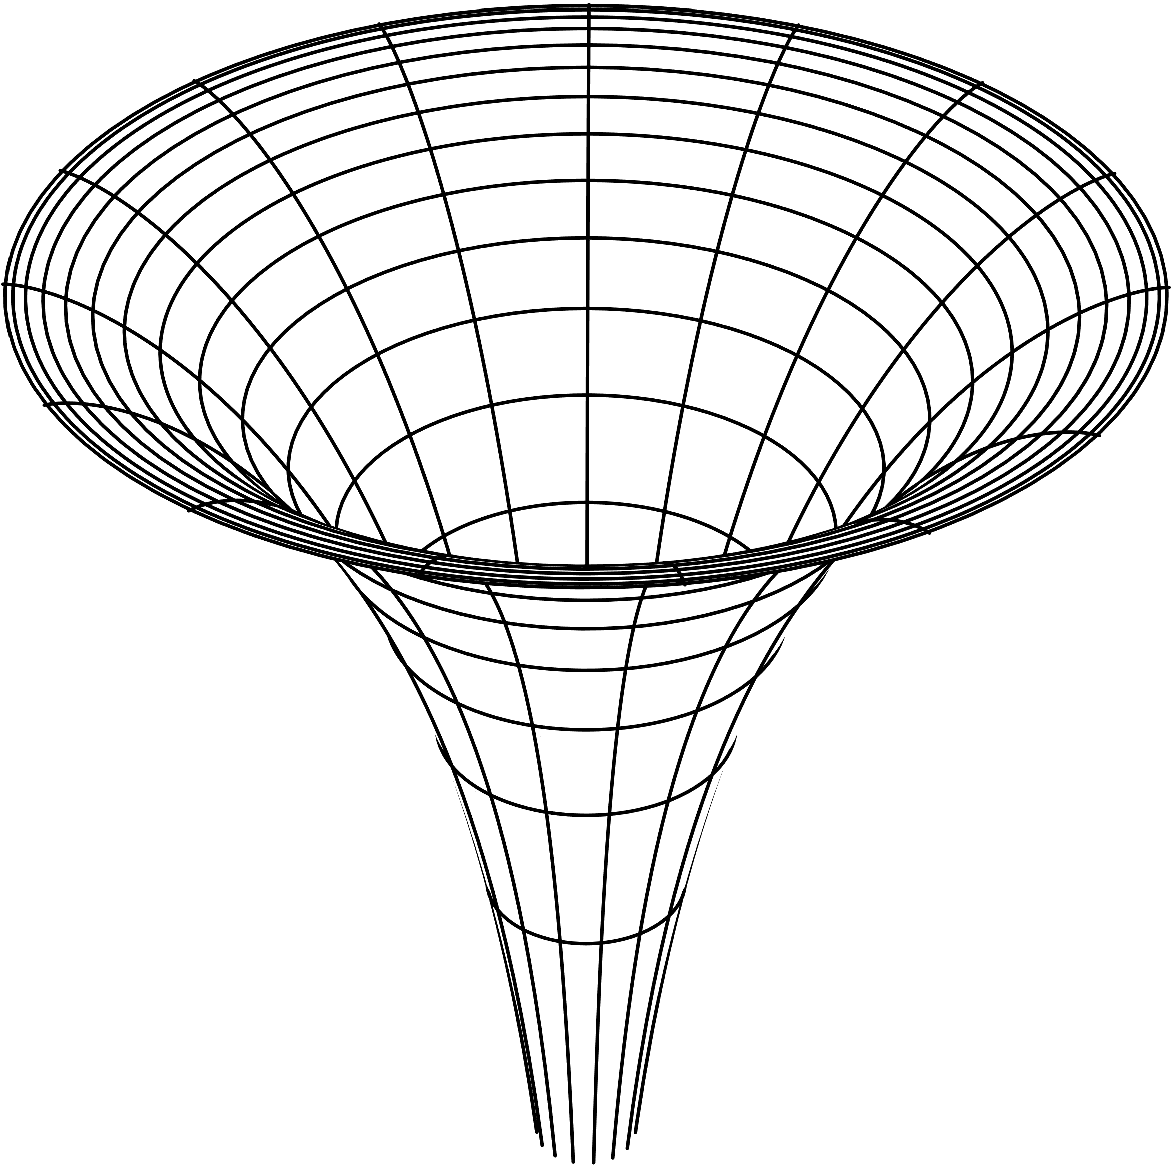
\includegraphics[width=6cm]{./img/Pseudosphere.pdf}
	\caption{Псевдосфера}
\end{figure}

\begin{solution}
	\begin{enumerate}[nolistsep, label=(\arabic*)]
		\item Напрямую вычисляем коэффициенты\footnotemark:
			\begin{gather*}
				\vec{r}_u = \br{a\cos u\cos v,\,a\cos u\sin v,\,a\ctg u\cos u},\quad \vec{r}_v = (-a\sin u\sin v,\,a\sin u\cos v, 0),\\
				g_{11} = \langle\vec{r}_u, \vec{r}_u\rangle = a^2\cos^2u\big(\underbrace{(\cos^2v + \sin^2v)}_1 + \ctg^2u\big) = a^2\cos^2u\underbrace{(1 + \ctg^2u)}_{1 / \sin^2u} = a^2\ctg^2u,\\
				g_{12} = \langle\vec{r}_v, \vec{r}_v\rangle = -\cancel{\frac{a^2}{4}\sin2u\sin2v} + \cancel{\frac{a^2}{4}\sin2u\sin2v} = 0,\\
				g_{22} = \langle\vec{r}_v, \vec{r}_v\rangle = a^2\sin^2u\underbrace{(\sin^2v + \sin^2v)}_1 = a^2\sin^2u.
			\end{gather*}%
			\footnotetext{Выкладка: $\ds\br{\ln\tg\frac{u}{2}}^\prime = \frac{1}{\tg\frac{u}{2}} \cdot \frac{1}{\cos^2\frac{u}{2}} \cdot \frac{1}{2} = \frac{1}{2\sin\frac{u}{2}\cos\frac{u}{2}} = \frac{1}{\sin u}$.}%
			Пишем первую квадратичную форму:
			\[
				\d s^2 = a^2\ctg^2u\d u^2 + a^2\sin^2u\d v^2.
			\]
		\item Считаем частные производные, пользуясь формулами Френе:
			\[
				\vec{r}_t = \vec{v} + \lambda\dot{\vec{n}} = \vec{v} + \lambda(-k\vec{v} + \varkappa\vec{b}) = (1 - k\lambda)\vec{v} + \varkappa\lambda\vec{b},\quad \vec{r}_\lambda = \vec{n}.
			\]
			Вычисляем коэффициенты первой квадратичной формы:
			\begin{gather*}
				g_{11} = \langle\vec{r}_t, \vec{r}_t\rangle = (1 - k\lambda)^2 + \varkappa^2\lambda^2,\\
				g_{12} = \langle\vec{r}_t, \vec{r}_\lambda\rangle = 0,\\
				g_{22} = \langle\vec{r}_\lambda, \vec{r}_\lambda\rangle = 1.
			\end{gather*}
			Итак, выписываем первую квадратичную форму:
			\[
				\d s^2 = \big((1 - k\lambda)^2 + \varkappa^2\lambda^2\big)\d t^2 + \d\lambda^2.
			\]
	\end{enumerate}
\end{solution}

\begin{problem}
	Найти угол между пересекающимися кривыми $u + v = 0$ и $u - v = 0$ на \textit{геликоиде} --- поверхности вида
	\[
		\vec{r}(u, v) = (u\sin v, u\cos v, av),
	\]
	где $u, v \in \R$, $a > 0$.
\end{problem}

\begin{figure}[H]
	\centering
	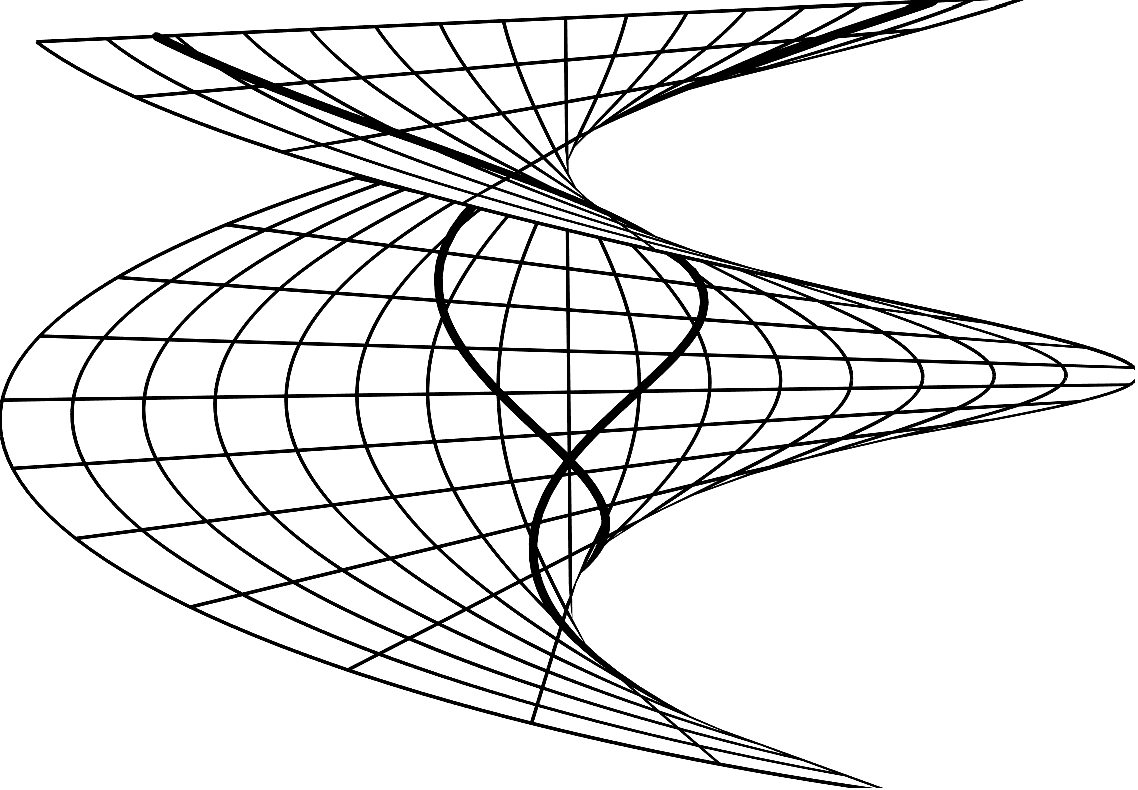
\includegraphics[width=6cm]{./img/HelicoidCurves.pdf}
	\caption{Две линии на геликоиде}
\end{figure}

\begin{solution}
	Посчитаем первую квадратичную форму нашей поверхности.
	\begin{gather*}
		\vec{r}_u = (\sin v, \cos v, 0),\quad \vec{r}_v = (u\cos v, -u\sin v, a),\\
		g_{11} = \langle\vec{r}_u, \vec{r}_u\rangle = {\underbrace{\sin^2v + \cos^2v}_{1}} = 1,\quad g_{12} = \langle\vec{r}_u, \vec{r}_v\rangle = 0,\\
		g_{22} = \langle\vec{r}_v, \vec{r}_v\rangle = u^2{\underbrace{(\sin^2v + \cos^2v)}_{1}} + a^2 = u^2 + a^2,\\
		\G(u, v) =
		\begin{pmatrix}
			1 & 0\\
			0 & u^2 + a^2
		\end{pmatrix}.
	\end{gather*}

	Данные кривые легко запараметризовать: $(t, -t)$ и $(t, t)$. Они пересекаются в точке $(0, 0)$. Их вектора скорости в этой точке есть $\vec{v}_1 = (1, -1)$ и $\vec{v}_2 = (1, 1)$ соответственно. Угол между кривыми находим по формуле
	\[
		\cos\angle(\vec{v}_1, \vec{v}_2) = \frac{\langle\vec{v}_1, \vec{v}_2\rangle|_{\G(0, 0)}}{\sqrt{\langle\vec{v}_1, \vec{v}_1\rangle|_{\G(0, 0)}}\sqrt{\langle\vec{v}_2, \vec{v}_2\rangle|_{\G(0, 0)}}} = \frac{1 - a^2}{1 + a^2}.
	\]
	Отсюда $\ds\angle(\vec{v}_1, \vec{v}_2) = \arccos\frac{1 - a^2}{1 + a^2}$.
\end{solution}

\begin{definition}
	\textit{Площадью} области $U$ на поверхности $\vec{r} = \vec{r}(u, v)$ называется величина
	\[
		\sigma(U) \vcentcolon = \iint\limits_{U}\sqrt{\deg\G}\d u\d v.
	\]
	(Здесь область $U$ задана параметрически координатами $u$ и $v$.)
\end{definition}

Это определение (как и определение длины кривой) принимается как данность. Мотивировка такого определения в том, что $\sqrt{\det\G}$ --- это (ориентированная) площадь параллелограмма, натянутого на касательные вектора $\vec{r}_u$ и $\vec{r}_v$. Естественно назвать выражение $\d\sigma \vcentcolon = \sqrt{\det\G}\d u\d v$ \textit{элементом площади}. Тогда определение площади принимает вид
\[
	\sigma(U) = \iint\limits_{U}\d\sigma.
\]

Площадь можно определить таким же образом не только на поверхности, но и в целом для римановой метрики в криволинейных координатах.

\begin{problem} \label{problem:AreaTriangle}
	В модели геометрии Лобачевского в верхней полуплоскости найти площадь треугольника, ограниченного кривыми
	\[
		x = 0,\quad (x - 1)^2 + y^2 = 4,\quad x^2 + y^2 = 9.
	\]
\end{problem}

\begin{solution}
	Метрика в модели геометрии Лобачевского в верхней полуплоскости имеет вид
	\[
		\d s^2 = \frac{\d x^2 + \d y^2}{y^2},
	\]
	и $\sqrt{\det\G(x, y)} = 1 / y^2$. Следовательно, площадь нашего треугольника равна
	\[
		\sigma(U) = \iint\limits_{U}\frac{1}{y^2}\d x\d y,
	\]
	что после перехода к повторному интегралу даёт выражение
	\begin{multline*}
		\sigma(U) = \int\limits_0^3 \d x\int\limits_{\sqrt{4 - (x - 1)^2}}^{\sqrt{9 - x^2}}\frac{1}{y^2}\d y = \int\limits_0^3\br{\frac{1}{\sqrt{4 - (x - 1)^2}} - \frac{1}{\sqrt{9 - x^2}}}\d x =\\ = \left.\br{\arcsin\frac{x - 1}{2} - \arcsin\frac{x}{3}}\right|_0^3 = 0 - \br{-\frac{\pi}{6}} = \frac{\pi}{6}.
	\end{multline*}

	\begin{figure}[H]
		\centering
		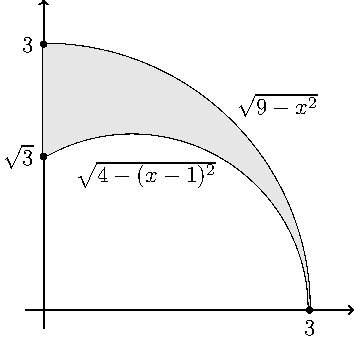
\includegraphics[width=6cm]{./img/CurveTriangle.pdf}
		\caption{Переход к повторному интегралу}
	\end{figure}
\end{solution}

\begin{example} В качестве доказательства пунктов $(2)$ и $(3)$ смотреть пример \ref{example:IFormOnSurfaces}.
	\begin{enumerate}[nolistsep, label=(\arabic*)]
		\item Если поверхность задана в параметрической форме $\vec{r} = \vec{r}(u, v)$ и $V$ --- такая область на плоскости $(u, v)$, что $\vec{r}(V) = U$, то
			\[
				\sigma(U) = \iint\limits_{V}\abs{\vec{r}_u \times \vec{r}_v}\d u\d v.
			\]
		\item Если поверхность задана как график функции $z = f(x, y)$ и область $U$ проектируется на область $V$ на плоскости $(x, y)$, то
			\[
				\sigma(U) = \iint\limits_{V}\sqrt{1 + f_x^2 + f_y^2}\d x\d y.
			\]
		\item Если поверхность задана уравнением $F(x, y, z) = 0$, $F_z \ne 0$ в области $U$, которая проектируется на область $V$ на плоскости $(x, y)$. Тогда
			\[
				\sigma(U) = \iint\limits_{V}\frac{\abs{\grad F}}{\abs{F_z}}\d x\d y.
			\]
	\end{enumerate}
\end{example}

\begin{problem}
	Найти площадь тора
	\[
		\begin{cases}
			x = (R + r\cos\psi)\cos\varphi,\\
			y = (R + r\cos\psi)\sin\varphi,\\
			z = r\sin\psi,
		\end{cases}
	\]
	где $r < R$, $0 \leqslant \varphi, \psi < 2\pi$.
\end{problem}

\begin{figure}[H]
	\centering
	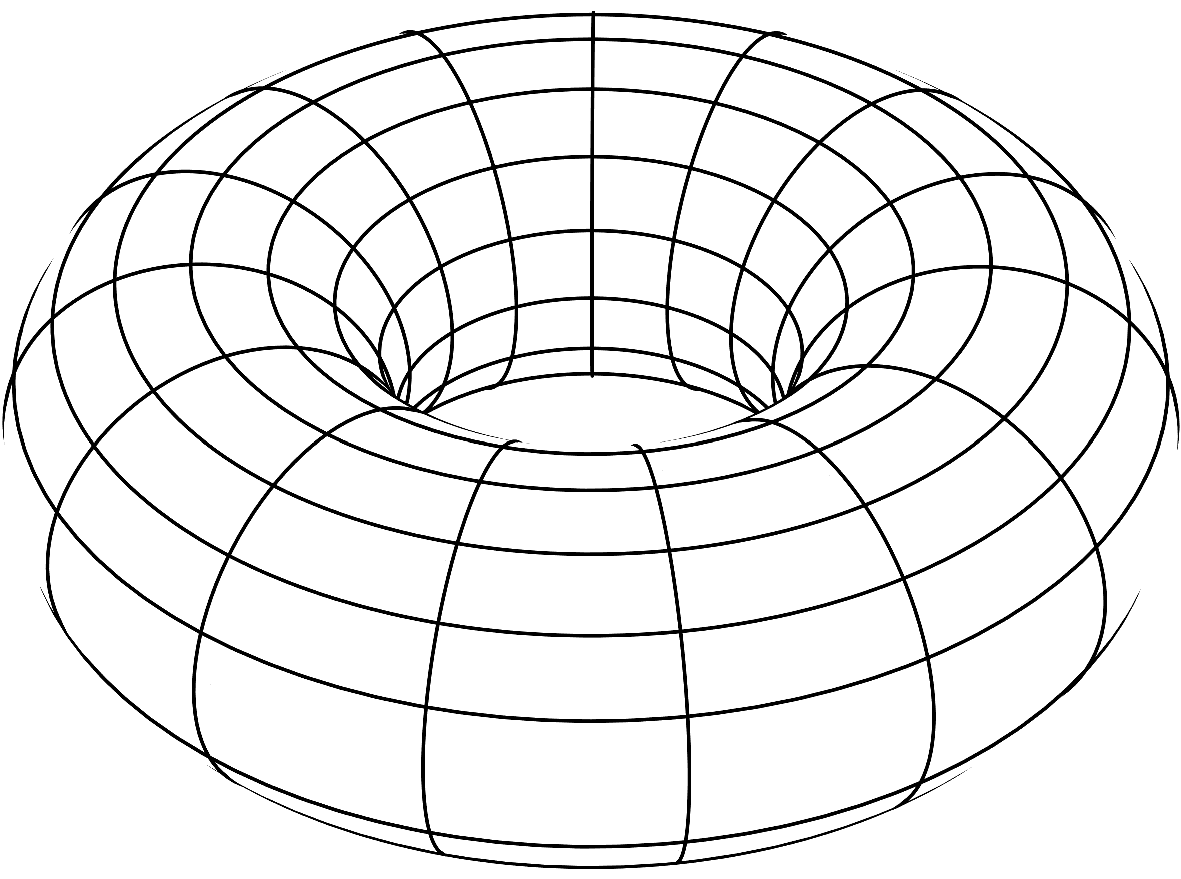
\includegraphics[width=6cm]{./img/Torus.pdf}
	\caption{Тор}
\end{figure}

\begin{solution}
	Находим частные производные радиус-вектора:
	\begin{gather*}
		\vec{r}_\varphi = (R + r\cos\psi)\big({-\sin\varphi}, \cos\varphi, 0\big),\\
		\vec{r}_\psi = r\big({-\cos\varphi\sin\psi}, -\sin\varphi\sin\psi, \cos\psi\big),
	\end{gather*}
	затем риманову метрику на торе:
	\[
		\G =
		\begin{pmatrix}
			(R + r\cos\psi)^2 & 0\\
			0 & r^2
		\end{pmatrix}.
	\]
	Считаем искомую площадь:
	\begin{multline*}
		\sigma = \iint\limits_{\varphi, \psi}\sqrt{\det\G}\d\varphi\d\psi = \int\limits_0^{2\pi}\d\varphi\int\limits_0^{2\pi}(R + r\cos\psi)r\d\psi =\\ = 2\pi r\int\limits_0^{2\pi}(R + r\cos\psi)\d\psi = 2\pi r \cdot 2\pi R = 4\pi^2 Rr.
	\end{multline*}
\end{solution}

Из существования натурального параметра на кривой следует, что каждый участок кривой можно отобразить в прямую с сохранением расстояний между точками. Двумерные поверхности в трехмерном евклидовом пространстве уже обладают внутренней геометрией. В общем случае никакая окрестность точки поверхности не может быть отображена на область в евклидовой плоскости с сохранением расстояний.

\begin{definition}
	Говорят, что поверхности $\M$ и $\mathcal{N}$ \textit{локально изометричны}, если в какой-то окрестности каждой точки первой поверхности существует диффеоморфизм $\vec{\varphi}\colon \M \to \mathcal{N}$, который сохраняет длины всех кривых. Сам дифферморфизм $\vec{\varphi}$ называется при этом \textit{локальной изометрией}.
\end{definition}

\noindent
Гладкое отображение поверхностей
\[
	\vec{f}\colon (u^1, u^2) \mapsto (\widetilde{u}^1(u^1, u^2), \widetilde{u}^2(u^1, u^2)),
\]
записанное в локальных координатах, сохраняет длины всех кривых, если и только если
\begin{equation} \label{eq:Isometry}
	\widetilde{g}_{ij}\big|_{\vec{f}(u^1, u^2)}\d\widetilde{u}^i\d\widetilde{u}^j = g_{kl}\big|_{(u^1, u^2)}\d u^k\d u^l,
\end{equation}
где $g_{kl}\d u^k\d u^l$ и $\widetilde{g}_{ij}\d\widetilde{u}^i\d\widetilde{u}^j$ --- первые квадратичные формы поверхностей. Идейно тут всё понятно --- это условие и означает, что на поверхностях <<одинаково измеряются расстояния>>. Распишем строго: пусть $\vec{\gamma}(t) = (u^1(t), u^2(t))$ --- кривая и $\widetilde{\vec{\gamma}}(t)$ --- её образ, $a \leqslant t \leqslant b$,
\[
	\int\limits_a^b\sqrt{g_{kl}(\vec{\gamma}(t))\,\dot{u}^k\dot{u}^l}\d t = \int\limits_a^b\sqrt{\widetilde{g}_{ij}(\widetilde{\vec{\gamma}}(t))\,\dot{\widetilde{u}}{}^i\dot{\widetilde{u}}{}^j}\d t.
\]

При локальной изометрии это равенство выполняется для любой кривой $\vec{r}(t)$, что равносильно соотношению \eqref{eq:Isometry}.

\begin{problem}
	Доказать, что \textit{геликоид}:
	\[
		\vec{r}(u, v) = (u\sin v, u\cos v, v),
	\]
	где $u, v \in \R$, локально изометричен \textit{катеноиду}:
	\[
		\widetilde{\vec{r}}(u, v) = (\ch u\cos v, \ch u\sin v, u),
	\]
	где $u \in \R$, $0 \leqslant v < 2\pi$.
\end{problem}

\begin{figure}[H]
	\centering
	\begin{minipage}{.4\textwidth}
		\centering
		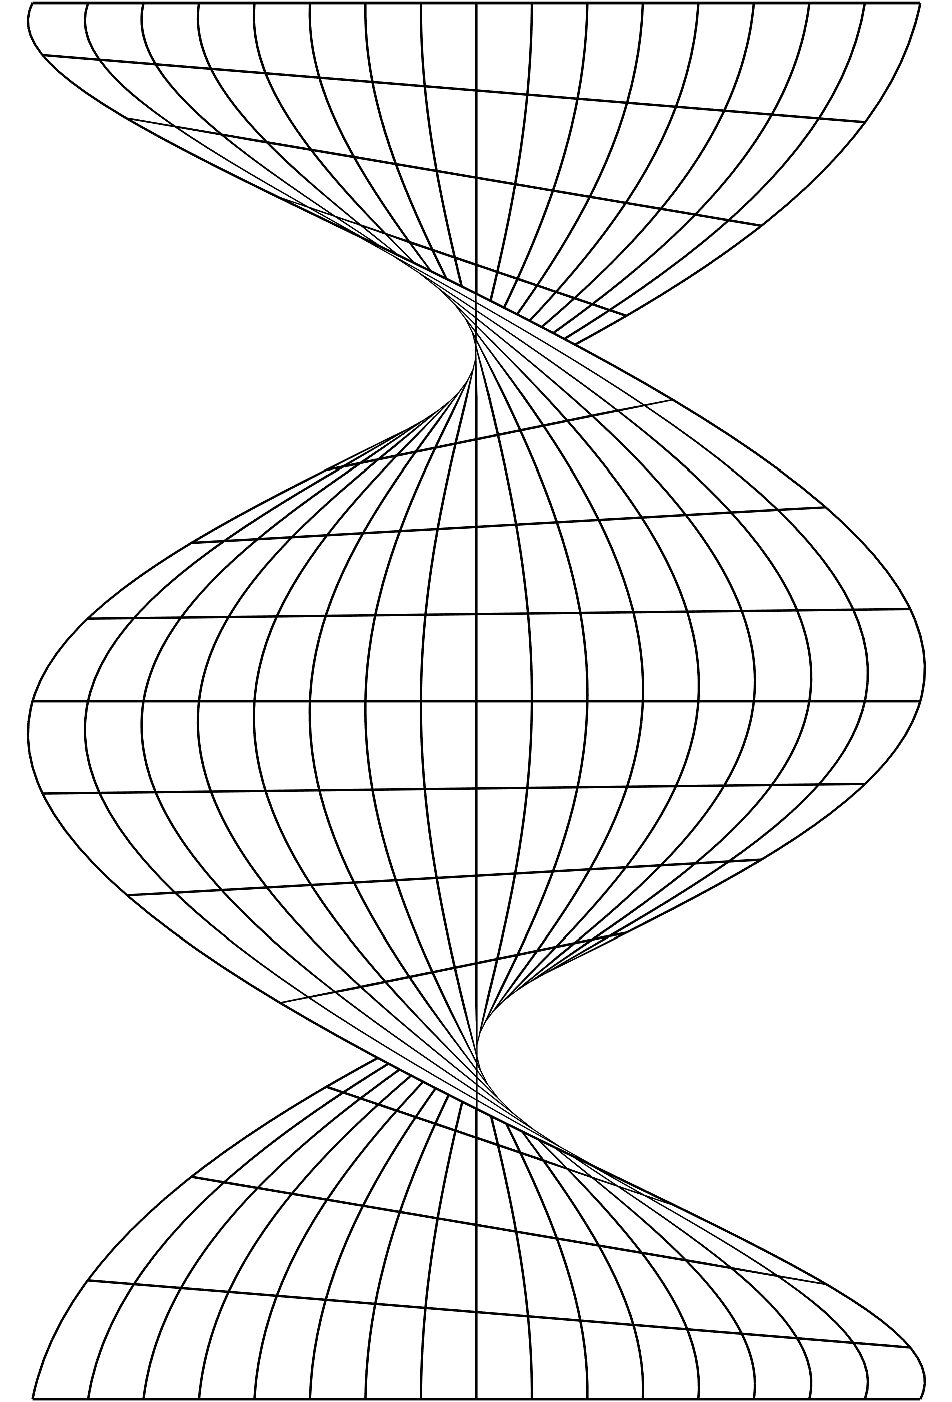
\includegraphics[width=5cm]{./img/Helicoid.pdf}
	\end{minipage}
	\begin{minipage}{.4\textwidth}
		\centering
		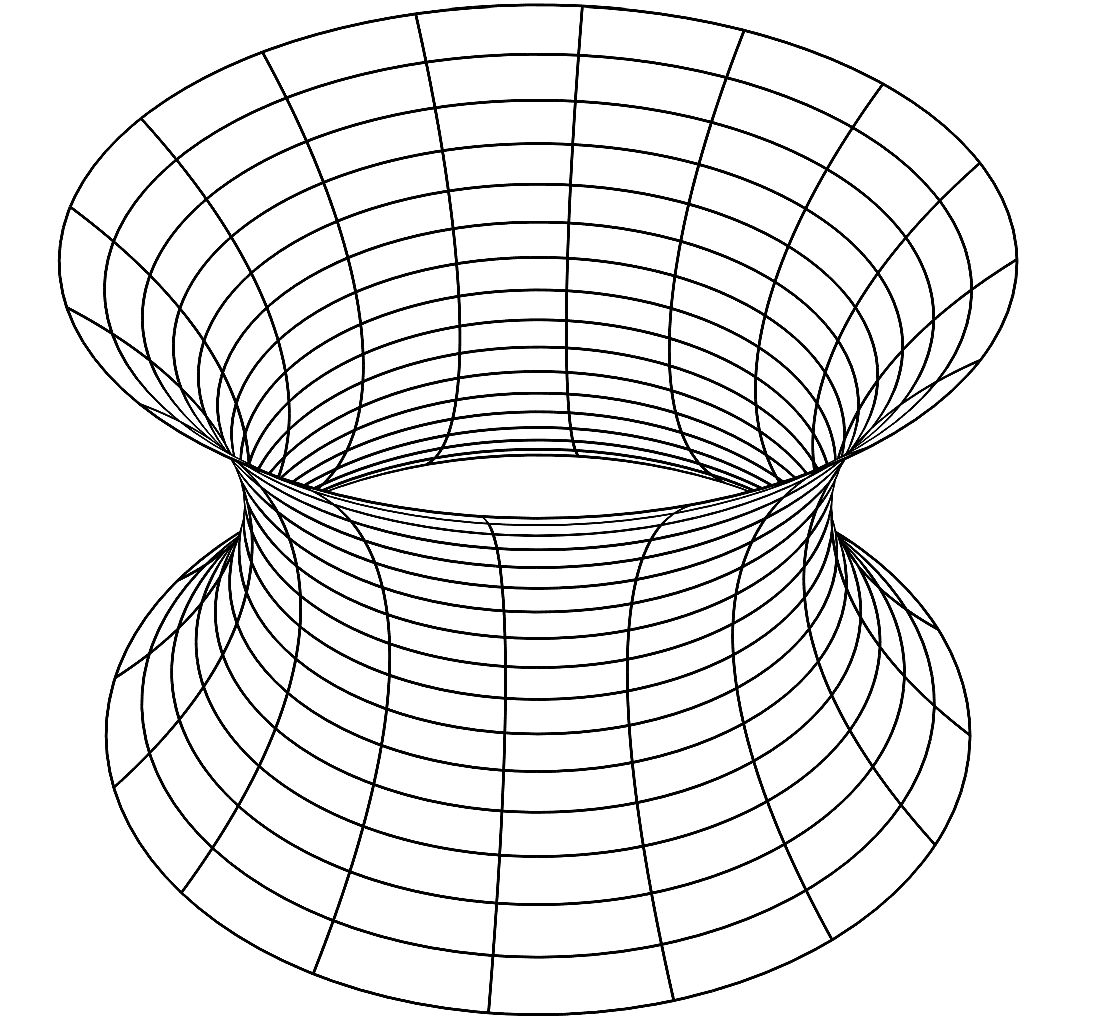
\includegraphics[width=5cm]{./img/Catenoid.pdf}
	\end{minipage}
	\vspace{.3cm}

	\begin{minipage}{.4\textwidth}
		\centering
		Геликоид
	\end{minipage}
	\begin{minipage}{.4\textwidth}
		\centering
		Катеноид
	\end{minipage}
	
	\caption[format=empty]{}
	\label{fig:HelicoidCatenoid}
\end{figure}

\begin{solution}
	Посчитаем первые квадратичные формы на наших поверхностях. Для геликоида:
	\begin{gather} \label{eq:HelicoidI}
		\vec{r}_u = (\sin v, \cos v, 0),\quad \vec{r}_v = (u\cos v, -u\sin v, 1),\nonumber\\
		g_{11} = \langle\vec{r}_u, \vec{r}_u\rangle = {\underbrace{\sin^2v + \cos^2v}_{1}} = 1,\quad g_{12} = \langle\vec{r}_u, \vec{r}_v\rangle = 0,\nonumber\\
		g_{22} = \langle\vec{r}_v, \vec{r}_v\rangle = u^2{\underbrace{(\sin^2v + \cos^2v)}_{1}} + 1 = u^2 + 1,\nonumber\\
		\d s^2 = \d u^2 + (u^2 + 1)\d v^2.
	\end{gather}
	Для катеноида:
	\begin{gather}
		\widetilde{\vec{r}}_{\widetilde{u}} = (\sh \widetilde{u}\cos \widetilde{v}, \sh \widetilde{u}\sin \widetilde{v}, 1),\quad \widetilde{\vec{r}}_{\widetilde{v}} = (-\ch \widetilde{u}\sin \widetilde{v}, \ch \widetilde{u}\cos \widetilde{v}, 0),\nonumber\\
		\widetilde{g}_{11} = \langle\widetilde{\vec{r}}_{\widetilde{u}}, \widetilde{\vec{r}}_{\widetilde{u}}\rangle = \sh^2\widetilde{u}\,{\underbrace{(\cos^2\widetilde{v} + \sin^2\widetilde{v})}_{1}} + 1 = \sh^2\widetilde{u} + 1 = \ch^2\widetilde{u},\nonumber\\
		\widetilde{g}_{12} = \langle\widetilde{\vec{r}}_{\widetilde{u}}, \widetilde{\vec{r}}_{\widetilde{v}}\rangle = 0,\quad
		\widetilde{g}_{22} = \langle\widetilde{\vec{r}}_{\widetilde{v}}, \widetilde{\vec{r}}_{\widetilde{v}}\rangle = \ch^2\widetilde{u}\,{\underbrace{(\sin^2\widetilde{v} + \cos^2\widetilde{v})}_{1}} = \ch^2\widetilde{u},\nonumber\\
		\d\widetilde{s}^2 = \ch^2\widetilde{u}\d\widetilde{u}^2 + \ch^2\widetilde{u}\d\widetilde{v}^2. \label{eq:CatenoidI}
	\end{gather}

	Согласно определению локальной изометрии, нам нужно в окрестности каждой точки предъявить диффеоморфизм, сохраняющий длины кривых. Попробуем найти <<глобальный>> диффеоморфизм такой, что форма \eqref{eq:HelicoidI} перейдёт в \eqref{eq:CatenoidI}. Мы хотим, чтобы было выполнено $\d u = \ch\widetilde{u}\d \widetilde{u}$. Проинтегрировав обе части, получаем $u = \sh\widetilde{u}$. Тогда можем взять $v = \widetilde{v}$, и получим
	\[
		\d u^2 = (\d\sh\widetilde{u})^2 = \ch^2\widetilde{u}^2\d\widetilde{u}^2,\quad(\sh^2\widetilde{u} + 1)\d\widetilde{v}^2 = \ch^2\widetilde{u}\d\widetilde{v}^2.
	\]
\end{solution}

\begin{problem}
	Доказать, что деформация гиперболического параболоида, определяемая следующими формулами, сохраняет площадь:
	\[
		\begin{cases}
			x = u,\\
			y = v,\\
			\ds z = \frac{1}{2}(u^2 - v^2)
		\end{cases}
		\mapsto
		\begin{cases}
			x = u,\\
			y = v,\\
			\ds z = \frac{\cos t}{2}(u^2 - v^2) + uv\sin t.
		\end{cases}
	\]
\end{problem}

\begin{solution}
	Проверим, что при данном преобразовании сохраняется форма площади. Метрика гиперболического параболоида задаётся матрицей
	\[
		\G_0 =
		\begin{pmatrix}
			1 + u^2 & -uv\\
			-uv & 1 + v^2
		\end{pmatrix}.
	\]
	(Эту матрицу легко выписать в уме, ведь поверхность по сути задана крафиком, а для такого задания мы уже выводили формулы в примере \ref{example:IFormOnSurfaces}). Форма площади есть
	\[
		\d\sigma = \sqrt{\G_0}\d u\d v = \sqrt{1 + u^2 + v^2}\d u\d v.
	\]
	Деформация, описанная в условии, даёт метрику
	\[
		\G_t =
		\begin{pmatrix}
			1 + (u\cos t + v\sin t)^2 & (u\cos t + v\sin t)(u\sin t - v\cos t)\\
			(u\cos t + v\sin t)(u\sin t - v\cos t) & 1 + (u\sin t - v\cos t)^2.
		\end{pmatrix}
	\]
	Легко видеть, что форма площади равна
	\[
		\d\sigma_t = \sqrt{\G_t}\d u\d v = \sqrt{1 + u^2 + v^2}\d u\d v.
	\]
	Итак, $\d\sigma = \d\sigma_t$ при любом $t$, так что данная деформация сохраняет площадь.
\end{solution}

% TODO: Написать про конформные отображения + условия Коши-Римана!

\subsection{Кривизна поверхности}

Сначала мы дадим <<дурацкое>> определение, а затем предоставим к нему исчерпывающую мотивацию. Рассмотрим поверхность, заданную параметрически: $\vec{r} = \vec{r}(u, v)$. Зададим к ней нормаль $\vec{n}$ в каждой точке:
\[
	\vec{n} \vcentcolon = \frac{\vec{r}_u \times \vec{r}_v}{\abs{\vec{r}_u \times \vec{r}_v}}.
\]

\begin{definition}
	\textit{Вторую квадратичную форму} определим как выражение
	\[
		L\d u^2 + 2M\d u\d v + N\d v^2,
	\]
	где
	\[
		L \vcentcolon = \langle\vec{r}_{uu}, \vec{n}\rangle,\quad M \vcentcolon = \langle\vec{r}_{uv}, \vec{n}\rangle,\quad N \vcentcolon = \langle\vec{r}_{vv}, \vec{n}\rangle.
	\]
	Полагая $u^1 = u$, $u^2 = v$, будем также записывать её в виде
	\[
		b_{ij}\d u^i\d u^j,
	\]
	где
	\[
		\B = \begin{pmatrix}
			b_{11} & b_{12}\\
			b_{12} & b_{22}
		\end{pmatrix} \vcentcolon =
		\begin{pmatrix}
			L & M\\
			M & N
		\end{pmatrix}.
	\]
\end{definition}

Для второй квадратичной формы, как и для первой, нужно доказать корректность определения --- то есть независимость от системы координат, в которой она записывается. Мы не будем утруждать себя лобовым доказательством тензорного закона, а увидим, что вторая квадратичная форма имеет геометрический смысл, инвариантный относительно выбора системы координат.

Рассмотрим кривую $\vec{\rho} = \vec{\rho}(u(t), v(t))$ на нашей поверхности, параметризованную в локальных координатах в окрестности точки $\vec{r}(u_0, v_0) \ni \Im\vec{\rho}$. Нормаль к поверхности в этой точке обозначим через $\vec{n}$. Тогда имеем (здесь через точку обозначена производная по $t$)
\begin{gather*}
	\ddot{\vec{\rho}} = \vec{\rho}_{uu}\dot{u}^2 + 2\vec{\rho}_{uv}\dot{u}\dot{v} + \vec{\rho}_{vv}\dot{v}^2 + \vec{\rho}_u\ddot{u} + \vec{\rho}_v\ddot{v},\\
	\langle\ddot{\vec{\rho}}, \vec{n}\rangle = L\dot{u}^2 + 2M\dot{u}\dot{v} + M\dot{v}^2,
\end{gather*}
так как $\vec{\rho}_u \perp \vec{n}$ и $\vec{\rho}_v \perp \vec{n}$. Получается, что значение второй квадратичной формы на векторе скорости кривой $\vec{\rho}$ (который, конечно же, является касательным вектором к поверхности) есть длина проекции вектора ускорения этой кривой на нормаль к поверхности.

Теперь имеем полное право называть определённое выше выражение квадратичной формой, обозначим её через $\II$. Попутно мы доказали следующее предложение.

\begin{proposition} \label{proposition:GeomII}
	Если $\vec{\rho} = \vec{\rho}(u(t), v(t))$ --- гладкая кривая на поверхности, то
	\[
		\langle\ddot{\vec{\rho}}, \vec{n}\rangle = \II(\dot{\vec{\rho}}).
	\]
\end{proposition}

\noindent%
Позже мы вернёмся к этому сюжету, но пока вынуждены отступить от него.

\subsection{Главные кривизны и нормальные сечения}

Подытожим наши рассуждения. В касательном пространстве к каждой точке поверхности определены две квадратичные формы --- $\I$ и $\II$, --- при этом форма $\I$ положительно определена. Из курса линейной алгебры известно, что тогда эти квадратичные формы можно привести к главным осям, то есть выбрать базис (в касательном пространстве), в котором матрица формы $\I$ будет единичной, а матрица формы $\II$ --- диагональной.

Кратно напомним, как это делать. Сначала нужно найти собственные значение пары квадратичных форм\footnotemark{}, то есть решить уравнение
\begin{equation} \label{eq:MainAxes}
	\det(\B - \lambda\G) = 0
\end{equation}
относительно $\lambda$, где $\G$ и $\B$ --- матрицы первой и второй квадратичной формы в каком-то базисе касательного пространства. Сразу отметим, что само уравнение \eqref{eq:MainAxes} инвариантно относительно замен координат и определяется самой поверхностью. Поэтому его коэффициенты в развёрнутом и приведённом виде
\[
	\lambda^2 -H\lambda + K = 0
\]
имеет смысл как-то обозначить.

\footnotetext{На самом деле, мы находим собственные значения линейного оператора $g^{ik}b_{kj}$, полученного поднятием индекса у второй квадратичной формы. Полезно держать это в голове.}

\begin{definition}
	Коэффициент $H$ называется \textit{средней кривизной} поверхности в данной точке\footnotemark, а коэффициент $K$ --- \textit{гауссовой кривизной}. Корни $\lambda_1$ и $\lambda_2$ уравнения \eqref{eq:MainAxes} называются \textit{главными кривизнами}. (По теореме Виета имеем $H = \lambda_1 + \lambda_2$, $K = \lambda_1\lambda_2$.)
\end{definition}

\footnotetext{<<Данная точка>> здесь --- это та, в касательном пространстве к которой мы сейчас находимся.}

Обычно среднюю кривизну определяют как среднее арифметическое главных кривизн, но такое определение влечёт лишь к небольшому усложнению формул за счёт возникновения множителя $1 / 2$. Все эти кривизны имеют для нас фундаментальное значение. Их очень глубокий геометрический смысл будет ясен позднее.

Если $\lambda_1 \ne \lambda_2$, то главные направления $\vec{\xi}_1$ и $\vec{\xi}_2$ ортогональны и находятся из уравнений
\[
	(\B - \lambda_iG)\vec{\xi}_i = \vec{0},
\]
где $i = 1, 2$.

А если $\lambda_1 = \lambda_2$, то первая и вторая квадратичные формы пропорциональны, и любые векторы подойдут как главные направления. Такие точки называются \textit{омбилическими}.

Лобовым раскрытием скобок можем получить явные формулы для гауссовой и средней кривизн через коэффициенты первой и второй квадратичных форм:
\[
	K = \frac{g_{11}g_{22} - g_{12}^2}{b_{11}b_{22} - b_{12}^2} = \frac{\det\G}{\det\B},\qquad H = \frac{g_{11}b_{22} + g_{22}b_{11} - 2g_{12}b_{12}}{g_{11}g_{22} - g_{12}^2} = \tr(\G^{-1}\B).
\]

\begin{example} \label{example:KonPlotSurface}
	Пусть поверхность задана как график функции $z = f(x, y)$. Тогда
	\begin{gather*}
		\vec{r}_x = (1, 0, f_x),\quad \vec{r}_{y} = (0, 1, f_y),\quad \vec{r}_x \times \vec{r}_y = (-f_x, -f_y, 1),\\
		\vec{r}_{xx} = (0, 0, f_{xx}),\quad \vec{r}_{xy} = (0, 0, f_{xy}),\quad \vec{r}_{yy} = (0, 0, f_{yy}),\\
		\vec{n} = \frac{\vec{r}_x \times \vec{r}_y}{\abs{\vec{r}_x \times \vec{r}_y}} = \frac{(-f_x, -f_y, 1)}{\sqrt{1 + f_x^2 + f_y^2}},\\
		b_{11} = \frac{f_{xx}}{\sqrt{1 + f_x^2 + f_y^2}},\quad b_{12} = \frac{f_{xy}}{\sqrt{1 + f_x^2 + f_y^2}},\quad b_{22} = \frac{f_{yy}}{\sqrt{1 + f_x^2 + f_y^2}}.
	\end{gather*}
	Отсюда, гауссова кривизна поверхности, заданной в виде графика, равна
	\[
		K = \frac{\det\G}{\det\B} = \frac{(1 + f_x^2)(1 + f_y^2) - f_x^2f_y^2}{(1 + f_x^2 + f_y^2)^2} = \frac{f_{xx}f_{yy} - f_{xy}^2}{(1 + f_x^2 + f_y^2)^2}.
	\]
\end{example}

\begin{problem} \label{problem:PseudosphereHK}
	Найти главные направления, гауссову и среднюю кривизны у псевдосферы
	\[
		x = a\sin u\cos v,\quad y = a\sin u\sin v,\quad z = a\br{\ln\tg\frac{u}{2} + \cos u},
	\]
	где $0 < u < \pi / 2$, $0 \leqslant v < 2\pi$, $a \ne 0$.
\end{problem}

\begin{solution}
	Первую квадратичную форму у псевдосферы мы уже считали в задаче \ref{problem:FindG}, получили
	\[
		\G =
		\begin{pmatrix}
			a^2\ctg^2u & 0\\
			0 & a^2\sin^2u
		\end{pmatrix}.
	\]

	Посчитаем вторую квадратичную форму. Для этого нам нужно считать вторые производные от параметризации $\vec{r}$ нашей поверхности. Первые, опять же, мы уже считали:
	\[
		\vec{r}_u = (a\cos u\cos v, a\cos u\sin v, a\ctg u\cos u),\quad\vec{r}_v = (-a\sin u\sin v, a\sin u\cos v, 0).
	\]
	Считаем вторые:
	\begin{gather*}
		\vec{r}_{uu} = \big({-a\sin u\cos v}, -a\sin u\sin v, -a\cos u(2 + \ctg^2u)\big),\\
		\vec{r}_{uv} = (-a\cos u\sin v, a\cos u\cos v, 0),\\
		\vec{r}_{vv} = (-a\sin u\cos v, -a\sin u\sin v, 0).
	\end{gather*}
	Находим вектор нормали:
	\begin{multline*}
		\vec{r}_u \times \vec{r}_v = \det
		\begin{pmatrix}
			\vec{e}_1 & \vec{e}_2 & \vec{e}_3\\
			a\cos u\cos v & a\cos u\sin v & a\ctg u\cos u\\
			-a\sin u\sin v & a\sin u\cos v & 0
		\end{pmatrix} =\\ = a^2 \br{{-\cos^2u\cos v}, -\cos^2u\sin v, \frac{1}{2}\sin 2u}.
	\end{multline*}
	\begin{multline*}
		\abs{\vec{r}_u \times \vec{r}_v}^2 = a^4{\cos^4u\underbrace{(\cos^2v + \sin^2v)}_{1}} + \frac{1}{4}a^4\sin^22u =\\ = a^4\big(\cos^4u + \cos^2u(1 - \cos^2u)\big) = a^4\cos^2u,
	\end{multline*}
	\begin{gather*}
		\vec{n} = \frac{\vec{r}_u \times \vec{r}_v}{\abs{\vec{r}_u \times \vec{r}_v}} = (-\cos u\cos v, -\cos u\sin v, \sin u).
	\end{gather*}
	Теперь можем найти коэффициенты второй квадратичной формы:
	\begin{multline*}
		b_{11} = \langle\vec{r}_{uu}, \vec{n}\rangle = {a\cos u\sin u\underbrace{(\cos^2 v + \sin ^2 v)}_{1}} - a\sin u\cos u(2 + \ctg^2u) =\\ = {-a\sin u\cos u\underbrace{(1 + \ctg^2 u)}_{1 / \sin^2u}} = -a\ctg u,
	\end{multline*}
	\begin{gather*}
		b_{12} = \langle\vec{r}_{uv}, \vec{n}\rangle = 0,\\
		b_{22} = \langle\vec{r}_{vv}, \vec{n}\rangle = {a\cos u\sin u\underbrace{(\cos^2 v + \sin ^2 v)}_{1}} = \frac{a}{2}\sin 2u.
	\end{gather*}
	Можем выписать матрицу второй квадратичной формы:
	\[
		\B =
		\begin{pmatrix}
			-a\ctg u & 0\\
			0 & \frac{a}{2}\sin 2u
		\end{pmatrix}.
	\]
	Находим главные кривизны:
	\begin{gather*}
		\det(\B - \lambda\G) = 0,\\
		\det
		\begin{pmatrix}
			-\ctg u - a\lambda \ctg^2u & 0\\
			0 & \frac{1}{2}\sin 2u - a\lambda \sin^2u
		\end{pmatrix} = 0,\\
		a^2\cos^2u \cdot \lambda^2 + a\br{{-\frac{\cos^3u}{\sin u}} + \cos u\sin u} \cdot \lambda -\cos^2 u = 0,\ \ \big|\ {:}\,a^2\cos^2u\\
		\lambda^2 - \frac{\ctg u - \tg u}{a}\lambda - \frac{1}{a^2} = 0.
	\end{gather*}

	Отсюда, $\lambda_1 = -a^{-1}\tg u$, $\lambda_2 = a^{-1}\ctg u$ и $H = a^{-1}(\ctg u - \tg u)$, $K \equiv -a^{-2}$. Наконец, можем найти главные направления.
	\begin{gather*}
		(\B - \lambda_1\G)\vec{\xi}_1 = \vec{0},\\
		\begin{pmatrix}
			0 & 0\\
			0 & \tg u
		\end{pmatrix}\vec{\xi}_1 = \vec{0}.
	\end{gather*}
	В качестве решения подойдёт, например, вектор $\vec{\xi}_1 = (1, 0)$. Ищем второй вектор:
	\begin{gather*}
		(\B - \lambda_2\G)\vec{\xi}_2 = \vec{0},\\
		\begin{pmatrix}
			-\frac{\cos u}{\sin^3 u} & 0\\
			0 & 0
		\end{pmatrix}\vec{\xi}_2 = \vec{0}.
	\end{gather*}

	Здесь подойдёт вектор $\vec{\xi}_2 = (0, 1)$. Итак, мы нашли главные направления в базисе $(\vec{r}_u, \vec{r}_v)$ касательного пространства. Можно записать их и в базисе $\R^3$, в котором находится наша поверхность. Для этого пишем $\vec{\xi}_i = \xi_i^1\vec{r}_u + \xi_i^2\vec{r}_v$. В данном случае всё очевидно --- $\vec{\xi}_1 = \vec{r}_u$, $\vec{\xi}_2 = \vec{r}_v$. Нам повезло, и векторы изначального базиса $(\vec{r}_u, \vec{r}_v)$ оказались главными направлениями. Так происходит редко, в общем случае мы найдём подходящие векторы, нормируем их и запишем в трёхмерных координатах.
\end{solution}

С каждой неомбилической точкой гладкой поверхности можно связать ортонормированный базис $(\vec{\xi}_1, \vec{\xi}_2, \vec{n})$ из главных направлений и вектора единичной нормали. Вблизи этой точки можно задать нашу функцию как график $z = f(x, y)$, к такому заданию поверхностей мы уже обращались в примере \ref{example:IFormOnSurfaces}. С одной стороны, первая квадратичная форма имеет вид
\[
	\begin{pmatrix}
		1 + f_x^2 & f_xf_y\\
		f_xf_y & 1 + f_y^2
	\end{pmatrix}.
\]

Но с другой стороны, в базисе из главных направлений матрица первой квадратичной формы в рассматриваемой точке единичная, отсюда находим $f_x = f_y = 0$. В выбранном базисе имеем $\vec{n} = (0, 0, 1)$, поэтому легко находим и коэффициенты второй квадратичной формы:
\[
	\begin{pmatrix}
		f_{xx} & f_{xy}\\
		f_{xy} & f_{yy}
	\end{pmatrix},
\]
при этом в выбранном базисе эта форма диагональна, то есть $f_{xy} = 0$. Таким образом, имеем следующие матрицы квадратичных форм:
\[
	\G =
	\begin{pmatrix}
		1 & 0\\
		0 & 1
	\end{pmatrix},\qquad
	\B =
	\begin{pmatrix}
		f_{xx} & 0\\
		0 & f_{yy}
	\end{pmatrix}.
\]

Сразу видим главные кривизны: $\lambda_1 = f_{xx}$, $\lambda_2 = f_{yy}$. Можно написать разложение функции $z = f(x, y)$ в ряд Тейлора, которое в нашем случае выглядит так:
\begin{equation} \label{eq:TailorII}
	z = \frac{\lambda_1}{2}x^2 + \frac{\lambda_2}{2}y^2 + \o(x^2 + y^2).
\end{equation}

Отбросив $\o(x^2 + y^2)$, мы получим уравнение параболоида, который приближает нашу поверхность вблизи начала координат. Эта соприкасающайся поверхность второго порядка служит аналогом соприкасающейся окружности к кривой. В зависимости от вида этой приближающей поверхности, каждую неомбилическую точку поверхности можно отнести к одному из трёх типов.

\begin{definition}
	\begin{enumerate}[nolistsep, label=(\arabic*)]
		\item Если $\lambda_1$ и $\lambda_2$ оба ненулевые и одного знака ($K > 0$), то такая точка называется \textit{эллиптической} (в этом случае приближающая поверхность --- эллиптический параболоид).
		\item Если $\lambda_1$ и $\lambda_2$ разных знаков ($K < 0$), то такая точка называется \textit{гиперболической} (приближающая поверхность --- гиперболический параболоид).
		\item Если одно из $\lambda_1$ и $\lambda_2$ нулевое ($K = 0$), то такая точка называется \textit{параболической} (приближающая поверхность --- параболический цилиндр).
	\end{enumerate}
\end{definition}

\begin{figure}[H]
	\centering
	\begin{minipage}{.3\textwidth}
		\centering
		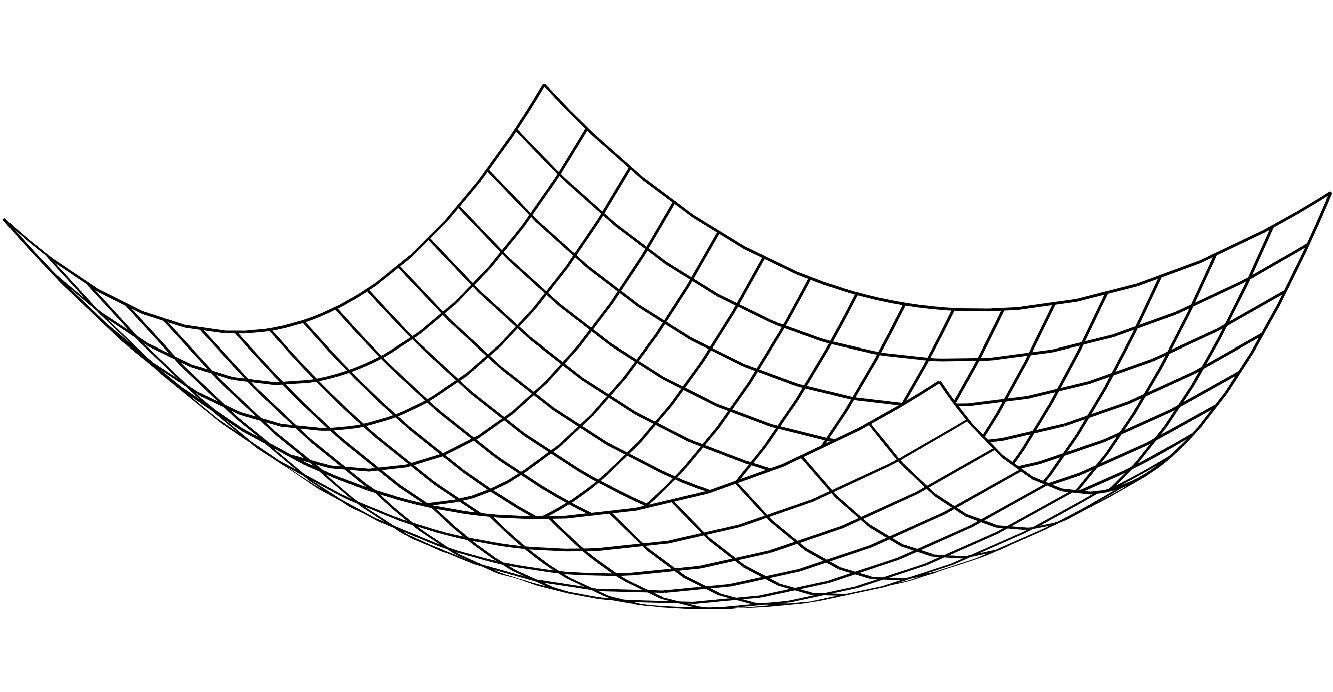
\includegraphics[height=2cm]{./img/Elliptic.pdf}

		$K > 0$
	\end{minipage}
	\begin{minipage}{.3\textwidth}
		\centering
		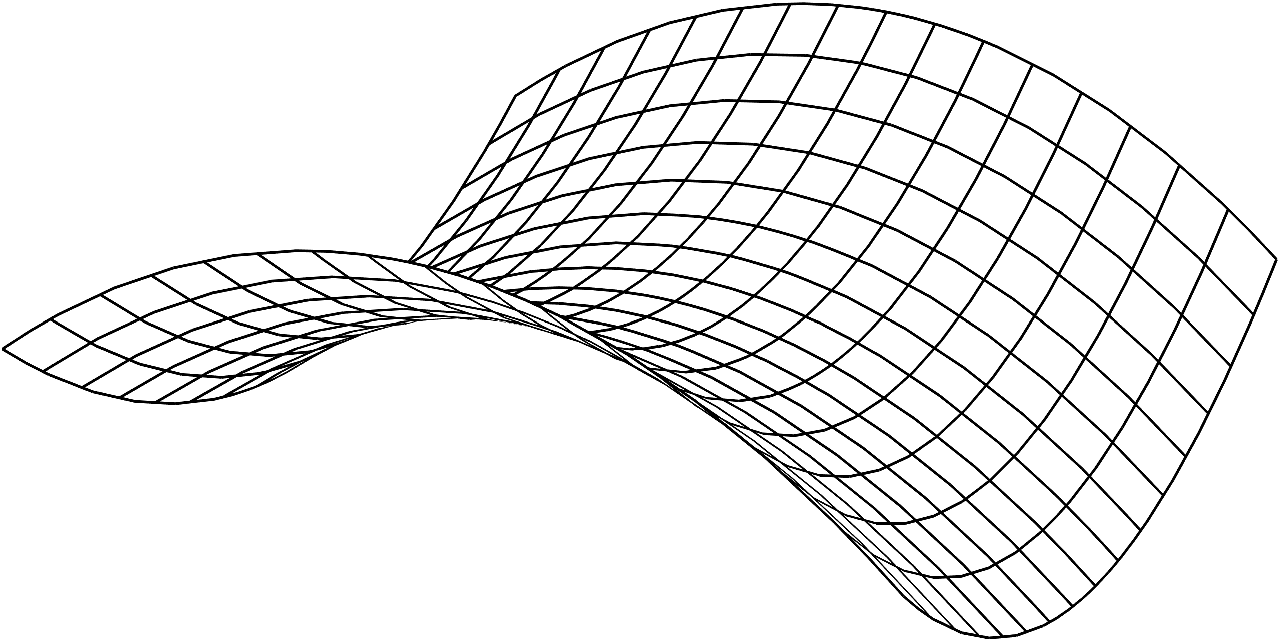
\includegraphics[height=2cm]{./img/Hyperbolic.pdf}

		$K < 0$
	\end{minipage}
	\begin{minipage}{.3\textwidth}
		\centering
		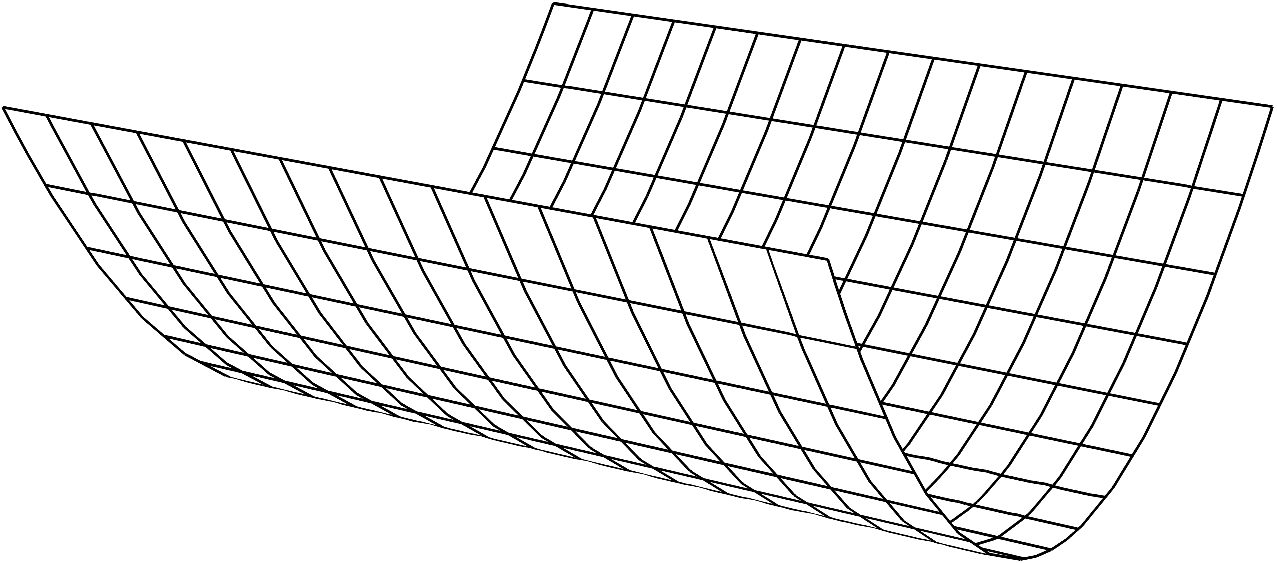
\includegraphics[height=2cm]{./img/Parabolic.pdf}

		$K = 0$
	\end{minipage}
	\caption{Вид соприкасающегося параболоида в зависимости от гауссовой кривизны}
\end{figure}

Далее мы опишем геометрический смысл главных кривизн и второй квадратичной формы, для этого мы будем рассматривать сечения поверхности плоскостями. 

\begin{definition}
	\textit{Нормальным сечением} поверхности $\M$ в некоторой точке $\vec{x} \in \M$ называется кривая в пересечении этой поверхности и плокости, порождённой каким-то касательным вектором $\vec{\xi} \in \T_{\vec{x}}\M$ и нормалью к поверхности в точке $\vec{x}$.
\end{definition}

 Обозначим через $\vec{n}_\rho$ вектор главной нормали кривой $\vec{\rho}$ в рассматриваемой точке, а через $\theta$ --- угол между ним и вектором нормали к поверхности, то есть $\theta = \angle(\vec{n}_\rho, \vec{n})$. Кривизна\footnotemark{} кривой $\vec{\rho}$ определяется из соотношения
\[
	\frac{\d^2\vec{\rho}}{\d s^2} = k\vec{n}_\rho,
\]
где $s$ --- натуральный параметр на кривой. Напишем
\[
	\left\langle\frac{\d^2\vec{\rho}}{\d s^2}, \vec{n}\right\rangle = b_{11}\br{\frac{\d u}{\d s}}^2 + 2b_{12}\frac{\d u}{\d s}\frac{\d v}{\d s} + b_{22}\br{\frac{\d v}{\d s}}^2 = \frac{b_{ij}\d u^i\d u^j}{\d s^2},
\]
причём $\d s^2 = \abs{\dot{\vec{\rho}}}^2\d t^2 = \I(\dot{\vec{\rho}})\d t^2$. Согласно предложению \ref{proposition:GeomII},
\[
	k\underbrace{\langle\vec{n}_\rho, \vec{n}\rangle}_{\cos\theta} = \left\langle\frac{\d^2\vec{\rho}}{\d s^2}, \vec{n}\right\rangle = \frac{b_{ij}\dot{u}^i\dot{u}^j}{\I(\dot{\vec{\rho}})} = \frac{\II(\dot{\vec{\rho}})}{\I(\dot{\vec{\rho}})},
\]
Таким образом, нами доказана следующая теорема.

\footnotetext{В этом разделе кривизны плоских сечений поверхностей будут пониматься в контексте кривизны со знаком, ведь они лежат в плоскости сечения, поэтому на них можно ввести коориентацию.}

\begin{theorem}
	Если кривая лежит на поверхности в $\R^3$, то произведение кривизны кривой на косинус угла между нормалью к поверхности и главной нормалью к кривой равно отношению значений второй и первой квадратичных форм на векторе скорости этой кривой.
\end{theorem}

\begin{corollary}[Теорема Менье] \label{theorem:Meusneir}
	Рассмотрим нормальное сечение поверхности $\M$, порождённое вектором $\vec{\xi} \in \T_{\vec{x}}\M$. Затем наклоним плоскость сечения вокруг вектора $\vec{\xi}$ на угол $\theta$ ($0 \leqslant \theta < \frac{\pi}{2}$). Кривизна в точке $\vec{x}$ получившегося сечения есть
	\[
		\frac{1}{\cos\theta}\frac{\II(\vec{\xi})}{\I(\vec{\xi})}.
	\]
\end{corollary}

\begin{figure}[H]
	\centering
	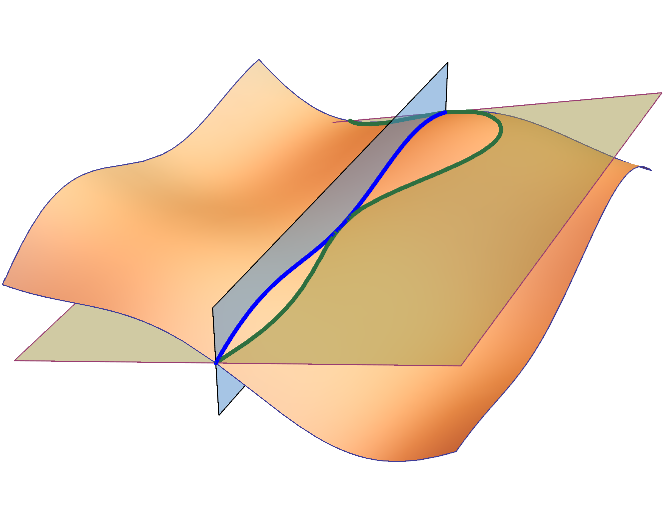
\includegraphics[width=8cm]{./img/ThetaSection.pdf}
	\caption{Нормальное сечение (синим) и сечение\\ наклонённой плоскостью (зелёным)}
\end{figure}

\noindent%
При $\theta = 0$ получаем кривизну нормального сечения:
\begin{equation} \label{eq:NormalCurvature}
	k_n = \frac{\II(\vec{\xi})}{\I(\vec{\xi})}.
\end{equation}
(Вообще, тут должен стоять $\pm$, но мы можем выбрать знак. Важно везде сделать это одинаково.) Кривизна сечения под углом $\theta$ выражается через кривизну нормального сечения:
\[
	k_{\theta} = \frac{k_n}{\cos\theta}.
\]
(Обычно теорему Менье формулируют именно в таком виде.)

Формула \ref{eq:NormalCurvature} даёт основной геометрический смысл второй квадратичной формы --- её значение на единичном касательном векторе есть кривизна нормального сечения, порождённого этим вектором. Итак, пусть имеем касательный вектор $\vec{\xi} = \xi^1\vec{\xi}_1 + \xi^2\vec{\xi}_2$, тогда:
\[
	k_{\vec{\xi}} = \frac{\II(\vec{\xi})}{\I(\vec{\xi})} = \frac{\lambda_1(\xi^1)^2 + \lambda_2(\xi^2)^2}{(\xi^1)^2 + (\xi^2)^2} = \lambda_1\cos^2\varphi + \lambda_2\sin^2\varphi,
\]
где $\varphi = \angle(\vec{\xi}, \vec{\xi}_1)$. Таким образом, нами доказана теорема.

\begin{theorem}[Формула Эйлера] \label{theorem:EulerFormula}
	Кривизна нормального сечения, порождённого касательным вектором $\vec{\xi}$, равна
	\[
		\lambda_1\cos^2\varphi + \lambda_2\sin^2\varphi,
	\]
	где $\lambda_1$ и $\lambda_2$ --- главные кривизны, а $\varphi$ --- угол между $\vec{\xi}$ и главным направлением $\vec{\xi}_1$.
\end{theorem}

Положим для определённости $\lambda_1 \leqslant \lambda_2$. Тогда главные кривизны $\lambda_1$ и $\lambda_2$ --- минимум и максимум, соответственно, кривизн нормальных сечений в рассматриваемой точке. (Функция $\lambda_1\cos^2\varphi + \lambda_2\cos^2\varphi$ определена на окружности, а окружность компактна, поэтому максимум и минимум достигаются.) При этом все значения между $\lambda_1$ и $\lambda_2$ достигаются в силу непрерывности. Отметим, что если $\lambda_1\lambda_2 \leqslant 0$, то существует нормальное сечение с нулевой кривизной, то есть прямая.

\begin{problem} \label{problem:EllipseCurvature}
	Найти кривизну эллипса с полуосями $a$ и $b$ (причём, $a < b$) в его вершинах.
\end{problem}

\begin{solution}
	Рассмотрим цилиндр $x^2 + y^2 = a^2$ и его плоское сечение под углом $\theta$ с плоскостью $z = 0$, где $\cos\theta = \frac{a}{b}$. Нормальное сечение есть окружность радиуса $a$, его кривизна равна $k_n = 1 / a$. Сечение наклонённой плоскостью есть эллипс с полуосями $a$ и $b$, согласно теореме Менье его кривизна в вершине, соответствующей большой полуоси, равна
	\[
		k_b = \frac{k_n}{\cos\theta} = \frac{b}{a^2}.
	\]
	Теперь рассмотрим его вершину, соответствующую меньшей полуоси. В ней нормальные сечения, соответствующие главным направлениям, есть прямая и окружность радиуса $1 / a$. Угол, соответствующий нашему сечению, есть $\theta$. Таким образом, по формуле Эйлера имеем
	\[
		k_a = \frac{1}{a}\cos^2\theta + 0\sin^2\theta = \frac{a}{b^2}.
	\]
\end{solution}

Легко видеть справедливость следующих двух следствий. Отметим, что первое из них может быть полезным для вычисления средней кривизны без подсчёта главных кривизн. Действительно, ведь значение второй квадратичной формы на единичном касательном векторе есть просто кривизна нормального сечения в направлении этого вектора, которую часто можно найти из геометрических соображений с помощью теоремы Менье.

\begin{corollary}
	Для любых ортогональных касательных единичных векторов $\vec{e}_1$, $\vec{e}_2$ выполнено $H = \II(\vec{e}_1) + \II(\vec{e}_2)$.
\end{corollary}

\begin{corollary}
	$\ds H = \frac{1}{\pi}\int\limits_0^{2\pi}k_{\vec{\xi}_1\cos\varphi\,+\,\vec{\xi}_2\sin\varphi}\d\varphi$.
\end{corollary}

Таким образом, средняя кривизна оправдывает своё название не только и даже не столько тем, что является удвоенным средним арифметическим главных кривизн. Она является удвоенным усреднённым значением по всем направлениям нормальной кривизны.

\begin{problem}
	На поверхности $z = 2z^2 + 9y^2$ найти среднюю кривизну в начале координат.
\end{problem}

\begin{solution}
	Данная поверхность является цилиндром над эллипсом
	\[
		\frac{(z - 1 / 4)^2}{1 / 16} + \frac{y^2}{1 / 72} = 1
	\]
	в плоскости $x = 0$. Нормальные сечения вдоль главных направлений в начале координат есть прямая и этот эллипс, так что средняя кривизна равна
	\[
		H = 0 + \frac{1 / 4}{1 / 72} = 18.
	\]
\end{solution}

\begin{problem}
	На поверхности $x^2 + y^2 - 2z^2 = 0$ найти среднюю кривизну в точке $(1, 1, 1)$.
\end{problem}

\begin{solution}
	Данная нам поверхность есть цилиндр. Нормальные сечения вдоль главных направлений в точке $(1, 1, 1)$ есть (образующая цилиндра) и некоторый эллипс. Можно геометрически искать полуоси этого эллипса, но мы поступим в духе решения задачи \ref{problem:EllipseCurvature}.

	Сечение конуса плоскостью $z = 1$ есть окружность $x^2 + y^2 = 2$, её кривизна равна $1 / \sqrt{2}$, а вектор её главной нормали в рассматриваемой точке направлена по вектору $\widetilde{\vec{n}} = \br{-1, -1, 0}$. Нормаль поверхности в данной точке имеет направление $\vec{n} = -\frac{1}{2}(\grad F)|_{(1, 1, 1)} = (-1, -1, 2)$. Косинус угла между плоскостями, содержащими эти сечения, равен
	\[
		\cos\theta = \frac{\langle\widetilde{\vec{n}}, \vec{n}\rangle}{\langle\widetilde{\vec{n}}, \widetilde{\vec{n}}\rangle\langle\vec{n}, \vec{n}\rangle} = \frac{2}{\sqrt{2} \sqrt{6}} = \frac{1}{\sqrt{3}}.
	\]
	По теореме Менье,
	\[
		k_{\theta} = \frac{1 / \sqrt{2}}{\cos\theta} = \frac{1}{\sqrt{6}}.
	\]
	Итак, средняя кривизна в рассматриваемой точке равна
	\[
		H = 0 + \frac{1}{\sqrt{6}} = \frac{1}{\sqrt{6}}.
	\]
\end{solution}

\subsection{Минимальные поверхности}

Этот раздел носит характер дополнительного, в нём мы рассмотрим один важный класс поверхностей. Для понимания происходящего следует сначала прочитать про деривационные формулы Гаусса "---Вайнгартена.

\begin{definition}
	Гладкая поверхность $\M$ называется \textit{минимальной}, если для любой её внутренней точки $\vec{x}$ найдётся такая окрестность $U$, что любая другая гладкая поверхность $\M^\prime$, совпадающая с $\M$ вне $U$ и имеющая тот же край $\partial\M^\prime = \partial\M$, имеет площадь не меньшую, чем $\M$.
\end{definition}

\begin{theorem}
	Поверхность минимальна тогда и только тогда, когда её средняя кривизна всюду равна нулю.
\end{theorem}

\begin{proof}
	Мы докажем только необходимость условия $H = 0$ для того, чтобы поверхность была минимальна.

	Пусть $\M$ --- минимальная поверхность, $\vec{x}$ --- её внутренняя точка, $\mathcal{N} \subset \M$ --- окрестность точки $\vec{x}$ на поверхности $\M$ такая, что площадь области $\mathcal{N}$ не меньше площади любой другой области с тем же краем.

	Выберем регулярную параметризацию $\vec{r}(u, v)$ на $\mathcal{N}$ и возьмём произвольную гладкую функцию $\varphi\colon \mathcal{N} \to \R$, обращающуюся в нуль вместе со своими производными на крае $\partial\mathcal{N}$, но такую, что $\varphi(\vec{x}) \ne 0$. Рассмотрим следующее семейство параметризованных поверхностей:
	\[
		\vec{r}_t(u, v) = \vec{r}(u, v) + t\varphi(u, v)\vec{n}(u, v),
	\]
	где $\vec{n}$, как обычно, --- вектор нормали. При каждом фиксированном $t$ из достаточно малой окрестности нуля эта формула задаёт регулярную параметризацию некоторой поверхности $\mathcal{N}_t$ с тем же краем, что и $\mathcal{N}$. Так что по построению $\sigma(\mathcal{N}_t) \geqslant \sigma(\mathcal{N})$. Напомним формулу для площади на поверхности:
	\[
		\sigma(\mathcal{N}) = \iint\limits_{\mathcal{N}}\sqrt{\det\G}\d u\d v,
	\]
	где $\G$ --- риманова метрика на поверхности $\mathcal{N}$. Для регулярной параметризации подынтегральное выражение гладко зависит от первых производных радиус-вектора $\vec{r}$ по $u$ и $v$, поэтому $\sigma(\mathcal{N}_t)$ --- гладкая функция от $t$. Будем понимать $g(t)$ определитель матрицы первой квадратичной формы поверхности $\mathcal{N}_t$. Далее хотим найти производную $\ds\frac{\partial}{\partial t}\sqrt{g}$.
	\[
		g_{ij}(t) = \langle\vec{r}_i + t(\varphi_i\vec{n} + \varphi\vec{n}_i) + \o(t), \vec{r}_j + t(\varphi_j\vec{n} + \varphi\vec{n}_j) + \o(t)\rangle = \langle\vec{r}_i + t\varphi\vec{n}_i, \vec{r}_j + t\varphi\vec{n}_j\rangle + \o(t)
	\]
	при $t \to 0$, поскольку $\vec{n} \perp \vec{r}_k$, $k = 1, 2$. Таким образом, $g(t)$ с точностью до $\o(t)$ есть матрица Грама векторов $\vec{r}_1 + t\varphi\vec{n}_1$, $\vec{r}_2 + t\varphi\vec{n}_2$, и выражается через них матрицей
	\[
		E + t\varphi C,
	\]
	где $C = -\G^{-1}\B$ --- матрица оператора Вайнгартена. (Это сразу следует из деривационных формул Вайнгартена.) Далее, вместо того, чтобы непосредственно вычислять $\sqrt{g(t)}$, вспомним, что эта величина равна площади параллелограмма, натянутого на соответствующую пару векторов, а отношение площадей равно абсолютной величине определителя соответствующей матрицы перехода, откуда
	\[
		\frac{\sqrt{g(t)}}{\sqrt{g(0)}} = \abs{\det(E + t\varphi C)} + \o(t) = 1 + t\varphi\tr C + \o(t) = 1 + t\varphi H + \o(t)
	\]
	как следствие теоремы \ref{theorem:Weingarten}. Отсюда получаем $\ds\frac{\partial}{\partial t}\sqrt{g}^\prime = \sqrt{\det \G}\varphi H$. Таким образом,
	\[
		\sigma(\mathcal{N}_t) = \sigma(\mathcal{N}) + t\iint\limits_{\mathcal{N}}\sqrt{\det \G}\varphi H\d u\d v + \o(t).
	\]
	Поскольку площадь поверхности $\mathcal{N}_t$ достигает минимума при $t = 0$ мы должны иметь
	\[
		0 = \left.\frac{d\sigma(\mathcal{N}_t)}{dt}\right|_{t = 0} = \iint\limits_{\mathcal{N}}\sqrt{\det \G}\varphi H\d u\d v
	\]
	при любом выборе функции $\varphi$. Покажем, что неравенство $H \ne 0$ ведёт к противоречию с этим условием. Возьмём новую функцию $\widetilde{\varphi} = \varphi^2H$. Получим
	\[
		\iint\limits_{\mathcal{N}}\sqrt{\det \G}\widetilde{\varphi}H\d u\d v = \iint\limits_{\mathcal{N}}\sqrt{\det\G}\varphi^2H^2\d u\d v > 0,
	\]
	так как подынтегральная функция неотрицательна, причём в точке $\vec{x}$ она положительна.
\end{proof}

Физический смысл минимальных поверхностей следующий. Если между двумя кривыми (или внутри одной замкнутой кривой) в пространстве натянуть мыльную плёнку, то она, стремясь всюду локально уменьшить свою площадь, примет форму минимальной поверхности. Самые простые примеры минимальных поверхностей --- плоскость, геликоид и катеноид (на геликоид и катеноид можно посмотреть на рисунке \ref{fig:HelicoidCatenoid}). В этом легко убедиться, посчитав их среднюю кривизну.

\begin{figure}[H]
	\centering
	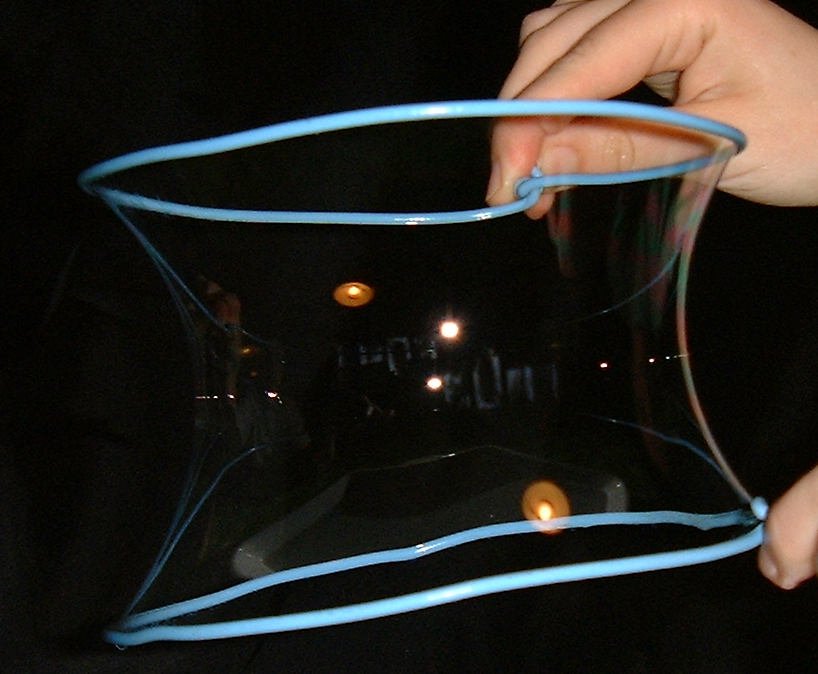
\includegraphics[width=6cm]{./img/Membrane.png}
	\caption{Мыльная плёнка принимает\\ форму катеноида}
\end{figure}

\subsection{Векторные поля на поверхностях}

\begin{definition}
	\textit{Векторным полем} на поверхности $\M$ называется отображение, которое каждой точке $\vec{x} \in \M$ ставит в соответствие вектор $\vec{v}(\vec{x})$ из касательной плоскости $\T_{\vec{x}}\M$. Векторное поле $\vec{v}$ называется \textit{гладким}, если в локальной параметризации коэффициенты $V^1$, $V^2$ разложения $\vec{v} = V^i\vec{r}_i$ вектора $\vec{v}$ по базису $\vec{r}_1$, $\vec{r}_2$ являются гладкими функциями.
\end{definition}

Отметим, что понятие гладкости векторного поля не зависит от выбора локальных координат, это сразу вытекает из теоремы о дифференцировании сложной функции.

С каждой локальной системой координат связаны два базисных векторных поля, определённых в соответствующей области на поверхности --- это $\vec{r}_1$ и $\vec{r}_2$. Их координаты по отношению к этой локальной системе постоянны: $(1, 0)$ и $(0, 1)$ соответственно. Зададим следующий вопрос: когда данная пара векторных полей $\vec{v}$, $\vec{w}$ может быть парой базисных векторных полей для некоторой локальной системы координат?

Разумеется, для начала нужно потребовать, чтобы $\vec{v}$ и $\vec{w}$ были линейно независимы в каждой точке. Однако этого, вообще говоря, недостаточно.

\begin{lemma} \label{lemma:WeakBasis}
	Пусть $\vec{e}_1$, $\vec{e}_2$ --- два единичных линейно независимых векторных поля на поверхности $\M$. Тогда в окрестности каждой точки $\vec{x}_0$ на поверхности $\M$ можно выбрать локальные координаты $(u^1, u^2)$ таким образом, чтобы $\vec{x}_0 = \vec{r}(0, 0)$, $\vec{r}_1 = \vec{e}_1$ при $u^2 = 0$ и $\vec{r}_2 = \vec{e}_2$ всюду в некоторой окрестности точки $\vec{x}_0$.
\end{lemma}

Иными словами, любая линейно независимая пара векторных полей задаёт базис на некоторой достаточно малой простой дуге в заданной окрестности, а большего в общем случае сказать не получается.

\begin{proof}
	Пусть $(u^1, u^2)$ --- произвольная система локальных координат в окрестности точки $\vec{x}_0$, причём $\vec{x}_0 = \vec{r}(u_0^1, u_0^2)$. Обозначим координаты векторов $\vec{e}_1$ и $\vec{e}_2$ по отношению к этой системе через $(E_1^1, E_1^2)$ и $(E_2^1, E_2^2)$ соответственно:
	\[
		\vec{e}_i = E^j_i\vec{r}_j.
	\]
	Решим уравнения
	\[
		\frac{d}{ds}\varphi^i(s) = E^i_1(\varphi^1(s), \varphi^2(s))
	\]
	с начальными условиями $\varphi^i(0) = u^i_0$ для $s$ из малой окрестности нуля. Геометрически это означает, что мы провели кривую $\gamma$ на поверхности $\M$ через точку $\vec{x}_0$ так, чтобы её вектором скорости в каждой точке $\vec{x}$ был вектор $\vec{e}_1(\vec{x})$. Параметр $s$ является натуральным на этой кривой (потому что поля единичные).

	Теперь для каждого фиксированного $s$, для которого определены функции $\varphi^1$ и $\varphi^2$, решим уравнения
	\[
		\frac{d}{dt}\psi^i = E^i_2(\psi^1, \psi^2)
	\]
	с начальными условиями $\psi^i|_{t = 0} = \varphi^i(s)$. Таким образом, $\psi^1$, $\psi^2$ --- функции двух аргументов, $s$ и $t$: $\psi^i = \psi^i(s, t)$. По теореме о гладкой зависимости решения обыкновенного дифференциального уравнения от начальных условий, $\psi^i(s, t)$ --- гладкие функции. По построению,
	\[
		\left.
		\begin{pmatrix}
			\begin{aligned}
				\frac{\partial\psi^1}{\partial s} \ \ \frac{\partial\psi^1}{\partial t}\\
				\frac{\partial\psi^2}{\partial s} \ \ \frac{\partial\psi^2}{\partial t}\\
			\end{aligned}
		\end{pmatrix}
		\right|_{(s, t) = (0, 0)} =
		\left.
		\begin{pmatrix}
			E_1^1 & E_2^1\\
			E_1^2 & E_2^2
		\end{pmatrix}
		\right|_{(u^1, u^2) = (u^1_0, u^2_0)}.
	\]

	Эта матрица невырожденна (потому что поля линейно независимы), поэтому локально можно сделать замену координат $u^1 = \psi^1(s, t)$, $u^2 = \psi^2(s, t)$. По построению будем иметь
	\begin{gather*}
		\frac{\partial}{\partial s}\vec{r}(\psi^1(s, t), \psi^2(s, t)) = (\vec{r}_iE_1^i)(\psi^1(s, t), \psi^2(s, t)) = \vec{e}_1(\psi^1(s, t), \psi^2(s, t))\ \text{при $t = 0$},\\
		\frac{\partial}{\partial t}\vec{r}(\psi^1(s, t), \psi^2(s, t)) = (\vec{r}_iE_2^i)(\psi^1(s, t), \psi^2(s, t)) = \vec{e}_2(\psi^1(s, t), \psi^2(s, t))\ \text{при всех $s$, $t$}.
	\end{gather*}
\end{proof}

Пусть гладкие векторные поля $\vec{v}$ и $\vec{w}$ линейно независимы в некоторой точке $\vec{x}_0$. Тогда они линейно независимы и в некоторой окрестности $U$ точки $\vec{x}_0$. Пусть $u^1$, $u^2$ --- некоторая локальная система координат в этой окрестности. Мы хотим выяснить, существует ли другая система координат $\widetilde{u}^1$, $\widetilde{u}^2$, для которой всюду в $U$ будет выполнено
\begin{equation} \label{eq:BasisVectorField}
	\frac{\partial}{\partial\widetilde{u}^1}\vec{r} = \vec{v},\quad \frac{\partial}{\partial\widetilde{u}^2}\vec{r} = \vec{w}.
\end{equation}
Найти такую систему координат $\widetilde{u}^1$, $\widetilde{u}^2$ означает найти функции перехода от неё к $u^1$, $u^2$ (или наоборот, что эквивалентно). Равенства \eqref{eq:BasisVectorField} равносильны следующим:
\[
	\frac{\partial u^i}{\partial \widetilde{u}^1}\vec{r}_i = V^i\vec{r}_i,\quad
	\frac{\partial u^i}{\partial \widetilde{u}^2}\vec{r}_i = W^i\vec{r}_i,
\]
то есть следующей системе из двух дифференциальных уравнений:
\[
	\begin{cases}
		\begin{aligned}
			& \frac{\partial u^i}{\partial\widetilde{u}^1} = V^i(u^1, u^2),\\
			& \frac{\partial u^i}{\partial\widetilde{u}^2} = W^i(u^1, u^2).
		\end{aligned}
	\end{cases}
\]
Выписываем для неё условие совместности \eqref{eq:Darboux}:
\[
	\frac{\partial V^i}{\partial u^j}W^j = \frac{\partial W^i}{\partial u^j}V^j.
\]

\begin{definition}
	Для двух векторных полей $\vec{v}$, $\vec{w}$ их \textit{коммутатором} называется векторное поле
	\[
		[\vec{v}, \vec{w}] = \br{V^j\frac{\partial W^i}{\partial u^j} - W^j\frac{\partial V^i}{\partial u^j}}\vec{r}_i.
	\]
	Если $[\vec{v}, \vec{w}] \equiv \vec{0}$, то говорят, что поля $\vec{v}$ и $\vec{w}$ \textit{коммутируют}.
\end{definition}

\begin{proposition}
	Определение коммутатора векторных полей корректно, то есть не зависит от выбора системы координат.
\end{proposition}

\begin{proof}
	Рассмотрим $\vec{v}$ и $\vec{w}$ как отображения $\M \to \R^3$. По определению дифференциала, имеем для этих отображений:
	\[
		d\vec{v}(\vec{w}) = \frac{\partial(V^i\vec{r}_i)}{\partial u^j}W^j = \br{\frac{\partial V^i}{\partial u^j}\vec{r}_i + V^i\vec{r}_{ij}}W^j.
	\]
	Аналогично,
	\[
		d\vec{w}(\vec{v}) = \br{\frac{\partial W^i}{\partial u^j}\vec{r}_i + W^i\vec{r}_{ij}}V^j.
	\]
	Отметим, что второе слагаемое в обоих случаях одно и то же. Отсюда,
	\[
		d\vec{w}(\vec{v}) - d\vec{v}(\vec{w}) = \br{V^j\frac{\partial W^i}{\partial u^j} - W^j\frac{\partial V^i}{\partial u^j}}\vec{r}_i = [\vec{v}, \vec{w}].
	\]

	Таким образом, мы выразили коммутатор $[\vec{v}, \vec{w}]$ через инвариантные величины $d\vec{w}(\vec{v})$ и $d\vec{v}(\vec{w})$. Отметим, что каждая из этих двух величин не задаёт, вообще говоря, касательного поля к поверхности.
\end{proof}

Используя введённое понятие коммутатора векторных полей, приведённое выше рассуждение резюмируется следующим образом.

\begin{theorem}
	Два векторных поля $\vec{v}$ и $\vec{w}$ являются базисными векторными полями для некоторой локальной системы координат тогда и только тогда, когда они линейно независимы и коммутируют.
\end{theorem}

\begin{definition}
	\textit{Производной функции $f\colon \M \to \R$ по направлению поля $\vec{v}$} называется новая функция $L_{\vec{v}}f\colon \M \to \R$, определяемая формулой $(L_{\vec{v}}f)(\vec{x}) \vcentcolon = L_{\vec{v}(\vec{x})}f$. Функция $L_{\vec{v}}f$ называется также \textit{производной Ли} функции $f$.
\end{definition}

Можно показать что оператор $L_{\vec{v}}L_{\vec{w}} - L_{\vec{w}}L_{\vec{v}}$ --- не второго порядка, как это кажется на первый взгляд, а первого, причём $L_{\vec{v}}L_{\vec{w}} - L_{\vec{w}}L_{\vec{v}} = L_{[\vec{v}, \vec{w}]}$. Так, например, определяется коммутатор векторных полей в книге \cite{A24}. (Из явной формулы для коммутатора, выведенной нами выше, сразу следует $[\vec{v}, \vec{w}]^k = L_{\vec{v}}W^k - L_{\vec{w}}V^k$.)

\begin{proposition}
	Коммутатор $[\dot, \dot]$ обладает следующими свойствами:
	\begin{enumerate}[nolistsep, label=(\arabic*)]
		\item $[\vec{v}, \vec{u} + \lambda\vec{w}] = [\vec{v}, \vec{u}] + \lambda[\vec{v}, \vec{w}]$, $\lambda \in \R$ (\textit{линейность});
		\item $[\vec{v}, \vec{w}] + [\vec{w}, \vec{v}] = \vec{0}$ (\textit{кососимметричность});
		\item $[[\vec{v}, \vec{u}], \vec{w}] + [[\vec{w}, \vec{v}], \vec{u}] + [[\vec{u}, \vec{w}], \vec{v}] = \vec{0}$.
	\end{enumerate}
\end{proposition}

\begin{proof}
	Явная проверка по выведенной выше формуле.
\end{proof}

\begin{definition}
	Линейное пространство с бинарной операцией, обладающей свойствами $(1)$ "---$(3)$, называется \textit{алгеброй Ли}.
\end{definition}

Таким образом, векторные поля с операцией коммутирования образуют алгебру Ли. Известными примерами алгебр Ли служат также пространство $\R^3$ с операцией векторного произведения и пространство линейных матриц $n \times n$ с коммутатором $[A, B] = AB - BA$.

\subsection{Про обозначения для частных производных}

Фраза, упомянутая в эпиграфе, была сказана Александром Александровичем на одном из семинаров в контексте неудачного выбора обозначений для частных производных. Аналогичное замечание я обнаружил в книге \cite{A24}, так что привожу его ниже.

При работе с частными производными нужно твёрдо понимать, что в самом их обозначении кроется опасность: частная производная функции $f$ по $x$ зависит не только от того, какая функция в рассматриваемой области принята за координату $x$, но в ещё большей мере от того, как выбраны прочие координаты. Например, на плоскости с координатами $(x, y)$ частная производная $\partial f / \partial x$ функции $y$ равна нулю, но частная производная $\partial f / \partial x$ по той же функции точки плоскости по той же переменной $x$ в системе координат $(x, z)$, где $z = x + y$, равна $-1$. Следовало бы писать $\partial f / \partial x|_{y = \const}$, $\partial f / \partial x|_{z = \const}$.


\section{Основные уравнения в теории поверхностей}

\subsection{Деривационные формулы}

На протяжении всего этого раздела следует держать в голове, что мы пишем уравнения для двумерных систем криволинейных на поверхностях (которые нам интересно изучать), но можем их написать для любой размерности. По этой причине мы всё время будем использовать тензорную запись.

Мы хотим написать для поверхностей что-то похожее на формулы Френе, то есть наша цель --- научиться дифференцировать векторы
\[
	\vec{r}_1 \vcentcolon = \frac{\partial\vec{r}}{\partial x^1}\quad\text{и}\quad
	\vec{r}_2 \vcentcolon = \frac{\partial\vec{r}}{\partial x^2},
\]
для этого нам будет удобно обозначить
\[
	\vec{r}_{ij} \vcentcolon = \frac{\partial^2\vec{r}}{\partial x^i\partial x^j}.
\]

Векторы $(\vec{r}_1, \vec{r}_2, \vec{n})$ образуют базис в каждой точке поверхности, поэтому каждый вектор $\vec{r}_{ij}$ в нём как-то записывается. Заметим, что коэффициент при $\vec{n}$ мы уже знаем --- это соответствующий элемент матрицы второй квадратичной формы $b_{ij}$. Действительно, ведь по определению $b_{ij} = \langle\vec{r}_{ij}, \vec{n}\rangle$.

\begin{definition}
	Коэффициенты $\Gamma_{ij}^k = \Gamma_{ji}^k$ в разложении
	\begin{equation} \label{eq:DerivativeGauss}
		\vec{r}_{ij} = \Gamma_{ij}^k\vec{r}_k + b_{ij}\vec{n}
	\end{equation}
	называются \textit{символами Кристоффеля}.
\end{definition}

\begin{lemma}[Тождества Кристоффеля]
	Символы Кристоффеля однозначно определяются метрикой на поверхности. Более точно, верна следующая формула:
	\begin{equation} \label{eq:ChristoffelIdentity}
		\Gamma_{ij}^k = \frac{g^{kl}}{2}\br{\frac{\partial g_{il}}{\partial x^j} + \frac{\partial g_{jl}}{\partial x^i} - \frac{\partial g_{ij}}{\partial x^l}},
	\end{equation}
	где $g^{kl}$ обозначают элементы матрицы $\G^{-1}$.
\end{lemma}

\begin{proof}
	Напишем
	\[
		\langle\vec{r}_{ij}, \vec{r}_l\rangle = \Gamma_{ij}^k\langle\vec{r}_k, \vec{r}_l\rangle = \Gamma_{ij}^kg_{kl}
	\]
	и
	\[\begin{tikzcd}
		{\ds\frac{\partial g_{il}}{\partial x^j}} & {\ds\frac{\partial}{\partial x^j}\langle\vec{r}_i, \vec{r}_l\rangle} & {\langle\vec{r}_{ij}, \vec{r}_l\rangle + \langle\vec{r}_i, \vec{r}_{jl}\rangle.}
		\arrow[equals, from=1-1, to=1-2]
		\arrow[equals, from=1-2, to=1-3]
	\end{tikzcd}\]
	Последнюю формулу напишем три раза, сдвигая координаты:
	\begin{gather*}
		\frac{\partial g_{il}}{\partial x^j} = \langle\vec{r}_{ij}, \vec{r}_l\rangle \phantom{{} + \langle\vec{r}_j, \vec{r}_{il}\rangle} + \langle\vec{r}_i, \vec{r}_{jl}\rangle,\\
		\frac{\partial g_{jl}}{\partial x^i} = \langle\vec{r}_{ij}, \vec{r}_l\rangle + \langle\vec{r}_j, \vec{r}_{il}\rangle \phantom{{} + \langle\vec{r}_i, \vec{r}_{jl}\rangle},\\
		\frac{\partial g_{ij}}{\partial x^l} = \phantom{\langle\vec{r}_{ij}, \vec{r}_l\rangle + {}} \langle\vec{r}_{il}, \vec{r}_j\rangle + \langle\vec{r}_i, \vec{r}_{jl}\rangle.
	\end{gather*}
	Сложим первые две строки из них и вычтем третью, получим
	\begin{gather*}
		\langle\vec{r}_{ij}, \vec{r}_l\rangle = \frac{1}{2}\br{\frac{\partial g_{il}}{\partial x^j} + \frac{\partial g_{jl}}{\partial x^i} - \frac{\partial g_{ij}}{\partial x^l}}.
	\end{gather*}
	Вспоминаем формулу, которую выписывали в начале этого доказательства, получаем
	\[
		g_{lk}\Gamma_{ij}^k = \frac{1}{2}\br{\frac{\partial g_{il}}{\partial x^j} + \frac{\partial g_{jl}}{\partial x^i} - \frac{\partial g_{ij}}{\partial x^l}}.
	\]
	Домножаем обе части на $g^{ml}$ и суммируем по $m$. Слева получим $g^{ml}g_{lk}\Gamma^k_{ij} = \delta^m_k\Gamma^k_{ij} = \Gamma^m_{ij}$:
	\[
		\Gamma_{ij}^m = \frac{g^{ml}}{2}\br{\frac{\partial g_{il}}{\partial x^j} + \frac{\partial g_{jl}}{\partial x^i} - \frac{\partial g_{ij}}{\partial x^l}}.
	\]
	Заменяем $m$ на $k$ и получаем ровно ту формулу, которую мы хотели доказать.
\end{proof}

Следует отметить, что символы Кристоффеля не задают никакого тензора в касательном пространстве к поверхности.

\begin{problem}
	Доказать, что при переходе к другим локальным координатам $(\widetilde{u}^1, \widetilde{u}^2)$ символы Кристоффеля преобразуются по следующему закону:
	\[
		\widetilde{\Gamma}_{ij}^k = \Gamma_{pq}^r\frac{\partial \widetilde{u}^k}{\partial \widetilde{u}^r}\frac{\partial u^p}{\partial \widetilde{u}^i}\frac{\partial u^q}{\partial \widetilde{u}^j} + \frac{\partial\widetilde{u}^k}{\partial u^p}\frac{\partial^2u^p}{\partial \widetilde{u}^i\partial \widetilde{u}^j}.
	\]
\end{problem}

\noindent
Формулы \eqref{eq:DerivativeGauss} с подстановкой \eqref{eq:ChristoffelIdentity} называются \textit{деривационными формулами Гаусса}.

Теперь хотим дифференцировать вектор $\vec{n}$. Обозначим
\[
	\vec{n}_1 \vcentcolon = \frac{\partial \vec{n}}{\partial x^1}\quad\text{и}\quad\vec{n}_2 \vcentcolon = \frac{\partial \vec{n}}{\partial x^2}.
\]

Поскольку вектор $\vec{n}$ имеет постоянную длину, оба этих вектора ортогональны $\vec{n}$, а значит, выражаются через базисные векторы $\vec{r}_1$, $\vec{r}_2$ касательного пространства в соответствующей точке. Пока напишем формально:
\begin{equation} \label{eq:DerivativeWeingarten}
	\vec{n}_i = c^j_i\vec{r}_j,
\end{equation}
позже мы придадим коэффициентам $c^j_i$ какой-то смысл.

\begin{lemma}
	Имеет место равенство
	\begin{equation} \label{eq:WeingartenIdentity}
		c^j_i = -g^{jk}b_{ki},
	\end{equation}
	где $g^{jk}$ обозначают элементы матрицы $\G^{-1}$.
\end{lemma}

\begin{proof}
	Векторы $\vec{n}$ и $\vec{r}_k$ ортогональны (по построению), поэтому
	\[
		\langle\vec{n}_i, \vec{r}_k\rangle = -\langle\vec{n}, \vec{r}_{ik}\rangle = -b_{ik}.
	\]
	Подставляя выражение для $n_i$, получаем
	\[
		c^j_i\langle\vec{r}_j, \vec{r}_k\rangle = c^j_ig_{jk} = -b_{ik}.
	\]
	Переписываем в матричном виде (с учётом $b_{ik} = b_{ki}$):
	\[
		GC = -B,\,\text{где }C = (c^j_i).
	\]
	Из него можно выразить матрицу $C$ как $C = -\G^{-1}\B$, или, в обозначениях Эйнштейна,
	\[
		c^j_i = -g^{jk}b_{ki}.
	\]
\end{proof}

\noindent
Уравнения \eqref{eq:DerivativeWeingarten} с подстановкой \eqref{eq:WeingartenIdentity} называются \textit{деривационными формулами Вайнгартена}.

Теперь обсудим смысл коэффициентов $c^j_i$. Разумеется, они зависят от параметризации. Но матрица $C$ преобразуется как матрица линейного оператора в касательном пространстве к поверхности, так как $C = -\G^{-1}\B$.

\begin{definition}
	\textit{Сферическим отображением} гладкой поверхности $\M$ называется отображение $\nu\colon \M \to S^2$, которое каждой точке $\vec{x}$ поверхности ставит в соответствие единичный вектор нормали $\vec{n}$ к соответствующей касательной плоскости $\T_{\vec{x}}\M$.
\end{definition}

\begin{proposition}
	Для любой точки $\vec{x}$ поверхности $\M$ касательные пространства $\T_{\vec{x}}\M$ и $\T_{\nu(\vec{x})}S^2$ совпадают.
\end{proposition}

\begin{proof}
	Вектор $\vec{\xi}$ лежит в касательном пространстве $\T_{\vec{x}}\M$ тогда и только тогда, когда $\vec{\xi} \perp \vec{n}$. При этом же условии он лежит в касательном пространстве $\T_{\nu(\vec{x})}S^2$.
\end{proof}

Последнее предложение означает, что дифференциал $d\nu|_{\vec{x}}$ сферического отображения можно понимать как линейный оператор на касательном пространстве.

\begin{theorem}
	Оператор $d\nu|_{\vec{x}}$ самосопряжён относительно скалярного произведения, заданного в $\T_{\vec{x}}\M$ первой квадратичной формой. Векторы главных направлений $\vec{\xi}_1$ и $\vec{\xi}_2$ являются для него собственными, а соответствующие им собственные значения суть главные кривизны, взятые с обратным знаком: $-\lambda_1$, $-\lambda_2$. Кроме того, имеют место равенства
	\[
		\det\br{d\nu|_{\vec{x}}} = \frac{\det\B}{\det\G} = K.
	\]
\end{theorem}

\noindent
Эта теорема доказывается прямой проверкой сразу из определений.


\section{Внутренняя геометрия поверхностей}

\subsection{Ковариантное дифференцирование, геодезические линии}

Мы хотим построить анализ на поверхности, который будет опираться только на её внутреннюю геометрию. В частности, мы хотим научиться дифференцировать векторные поля. Пусть на поверхности задано векторное поле $\vec{v}(t)$, гладко зависящее от времени. Обычное дифференцирование $\frac{d\vec{v}}{dt}$ нам не подойдёт, потому что такие векторы не обязательно касательные, так что на них нельзя смотреть с точки зрения внутренней геометрии поверхности. Нам нужно как-то модифицировать это определение.

Для правильного подхода нам стоит ответить на вопрос: какой разумный смысл можно придать словам <<идти прямо>> на поверхности? Хороший подход следующий --- положим на поверхность бусинку (которая не будет с неё слетать) и приведём её в движение без воздействия каких-либо внешних сил. Логично сказать, что тогда бусинка будет <<двигаться прямо>> по поверхности, при этом на неё действует лишь сила нормальной реакции, всюду перпендикулярная поверхности. Так, мы естественно пришли к следующему определению.

\begin{definition}
	\textit{Ковариантной производной} векторного поля $\vec{v}(t)$ по направлению (постоянного) касательного поля $\vec{w}$ называется векторное поле
	\[
		\big(\nabla_{\vec{w}}\vec{v}\big)(\vec{x}) \vcentcolon = \proj_{\vec{w}(\vec{x})}\frac{d\vec{v}}{dt}.
	\]
	\textit{Частными ковариантными производными} назовём ковариантные производные вдоль базисных векторных полей $\vec{r}_i$:
	\[
		\big(\nabla_i\vec{v}\big)(\vec{x}) = \proj_{\vec{r}_i(\vec{x})}\frac{d\vec{v}}{dt}.
	\]
\end{definition}

\noindent
Отметим, что проекция --- линейная операция, а потому выполнено
\[
	\nabla_{\vec{w}}\vec{v} = W^i\nabla_i\vec{v},
\]
так что ковариантная производная вдоль векторного поля однозначно определяется частными ковариантными производными, так что кажется уместным вывести общие формулы для частных ковариантных производных. Сначала найдём обычные частные производные векторного поля $\vec{r}$ по направлениям векторов $\vec{r}_i$:
\begin{equation} \label{eq:PartialVectorField}
	\partial_i\vec{v} = \frac{\partial V^k}{\partial u^i}\vec{r}_k + V^j\vec{r}_{ij} \stackrel{\eqref{eq:DerivativeGauss}}{=\joinrel=} \frac{\partial V^k}{\partial u^i}\vec{r}_k + V^j(\Gamma_{ij}^k\vec{r}_k + b_{ij}\vec{n}).
\end{equation}

Мы знаем, что $\big(\nabla_i\vec{v}\big)(\vec{x}) = \proj_{\T_{\vec{x}}\M}\partial_i\vec{v}$. Спроектировать на касательное пространство частные производные \eqref{eq:PartialVectorField} --- значит убрать у них слагаемые с $\vec{n}$. Получаем:
\[
	\nabla_i\vec{v} = \br{\frac{\partial V^k}{\partial u^i} + \Gamma_{ij}^kV^j}\vec{r}_k.
\]
Часто эту формулу записывают так:
\begin{equation} \label{eq:CovariantVectorField}
	\big(\nabla_i\vec{v}\big)^k = \frac{\partial V^k}{\partial u^i} + \Gamma_{ij}^kV^j
\end{equation}

Выбор коэффициентов $\Gamma_{ij}^k$ так, чтобы выражение \eqref{eq:CovariantVectorField} не зависело от выбора системы координат, называется \textit{связностью} (на многообразии). Определяя $\Gamma_{ij}^k$ как символы Кристоффеля, то есть по тождествам \eqref{eq:ChristoffelIdentity}, мы получаем \textit{симметричную риманову связность}. В этом курсе мы будем сталкиваться только с ней.

Итак, общая формула ковариантной производной имеет вид
\begin{equation} \label{eq:CovariantFormula}
	\big(\nabla_{\vec{w}}\vec{v}\big)^k = \big(W^i\nabla_i\vec{v}\big)^k = W^i\frac{\partial V^k}{\partial u^i} + \Gamma_{ij}^kW^iV^j.
\end{equation}

Мы поняли, что <<движением прямо>> вдоль некоторого векторного поля $\vec{w}$ мы хотим называть такое движение, что наша ковариантная производная вдоль этого векторного поля всюду равна нулю. Получаем систему уравнений $\big(\nabla_{\vec{w}}\vec{v}\big)^k = 0$ или, если расписать по формулам \eqref{eq:CovariantFormula},
\[
	W^i\frac{\partial V^k}{\partial u^i} + \Gamma_{ij}^kW^iV^j = 0.
\]

Видим, что это система дифференциальных уравнений первого порядка на $\vec{v}$. Из теоремы о существовании и единственности мы знаем, что она имеет единственное решение при любых начальных условиях. А начальные условия здесь --- это касательный вектор в момент времени $t = 0$: $\vec{v}(0) = \vec{\xi}$. Таким образом, мы определили операцию \textit{параллельного переноса} вектора $\vec{\xi}$ вдоль векторного поля $\vec{w}$. Однако нас, как правило, будет интересовать конкретный частный случай, когда векторное поле, вдоль которого мы будем осуществлять параллельный перенос образовано векторами скорости регулярной кривой на поверхности.

Векторы скорости произвольной регулярной кривой $\vec{\gamma}(t) = (u^1(t), u^2(t))$ на поверхности задают на этой кривой гладкое векторное поле, так что мы можем ковариантно дифференцировать вдоль кривой:
\[
	\nabla_{\dot{\vec{\gamma}}}\vec{v} = \dot{\gamma}^i\nabla_i\vec{v}.
\]
Подставим сюда формулы \eqref{eq:CovariantFormula}:
\[
	\big(\nabla_{\dot{\vec{\gamma}}}\vec{v}\big)^k = \big(\dot{\gamma}^i\nabla_i\vec{v}\big)^k = \dot{\gamma}^i\frac{\partial V^k}{\partial u^i} + \dot{\gamma}^i\Gamma_{ij}^kV^j = \frac{dV^k}{dt} + \dot{\gamma}^i\Gamma_{ij}^kV^j.
\]

\begin{definition}
	\textit{Параллельным переносом} вектора $\vec{\xi}$ вдоль кривой $\vec{\gamma}(t)$ называется векторное поле $\vec{v}(t)$, для которого $\vec{v}(0) = \vec{\xi}$ и $\nabla_{\dot{\vec{\gamma}}}\vec{\xi} \equiv \vec{0}$:
	\begin{equation} \label{eq:ParallelTranslation}
		\frac{dV^k}{dt} + \Gamma_{ij}^k\dot{\gamma}^iV^j = 0.
	\end{equation}
	Уравнения \eqref{eq:ParallelTranslation} при этом называются \textit{уравнениями параллельного переноса}.
\end{definition}

\begin{problem}
	На какой угол повернётся касательный вектор к сфере
	\begin{gather*}
		x = r\cos\varphi\cos\theta,\quad y = r\cos\varphi\sin\theta,\quad z = r\sin\varphi,\\
		-\pi / 2 \leqslant \varphi \leqslant \pi / 2,\quad 0 \leqslant \theta < 2\pi,\quad r \ne 0,
	\end{gather*}
	после параллельного переноса вдоль параллели $\theta = \theta_0$ на угол $\alpha$?
\end{problem}

\begin{solution}
	Появится здесь чуть позже.
\end{solution}

\begin{definition}
	Кривая $\vec{\gamma}(t)$ называется \textit{геодезической}, если $\nabla_{\dot{\vec{\gamma}}}\dot{\vec{\gamma}} \equiv \vec{0}$:
	\begin{equation} \label{eq:Geodesic}
		\ddot{\gamma}^k + \Gamma_{ij}^k\dot{\gamma}^i\dot\gamma^j = 0.
	\end{equation}
	Уравнения \eqref{eq:Geodesic} называт \textit{уравнениями геодезической}.
\end{definition}

Геодезические --- это как раз те кривые, которые будет проходить муравей, если его посадить на поверхность и попросить <<идти прямо>>. Отметим, что уравнения \eqref{eq:Geodesic} --- это дифференциальные уравнения уже \underline{второго} порядка, а потому начальными условиями для него служать начальная точка $\vec{\gamma}(0)$ и начальный вектор скорости $\dot{\vec{\gamma}}(0)$ --- куда посадить муравья и в какую сторону попросить его пойти.




\section{Дополнения}

\subsection{Модели плоскости Лобачевского}

Ближе к концу предыдущего раздела мы классифицировали поверхности с постоянной гауссовой кривизной. Заметим, что для $K \geqslant 0$ мы можем предъявить поверхность без края, гауссова кривизна которой всюду равна $K$. Для $K > 0$ это сфера радиуса $1 / \sqrt{K}$, а для $K = 0$ --- плоскость (<<сфера бесконечного радиуса>>).

Гильберт доказал, что гладкие поверхности постоянной отрицательной гауссовой кривизны в евклидовом пространстве $\R^3$ не могут быть полными, что в контексте настоящего курса означает, что любая такая поверхность обязательно имеет край. (Со схемой доказательства теоремы Гильберта можно ознакомиться в \S 4{.}4 книги \cite{NT14}.) Однако существует способ построить не имеющий края аналог сферы с постоянной отрицательной кривизной, если отказаться от евклидовости пространства $\R^3$.

Рассмотрим псевдоевклидово пространство $\R^{2, 1}$, скалярное произведение $\langle\cdot, \cdot\rangle$ в котором задано матрицей
\begin{equation*}
	\G =
	\begin{pmatrix}
		1 & 0 & 0\\
		0 & 1 & 0\\
		0 & 0 & -1
	\end{pmatrix}.
\end{equation*}

\noindent
В этом пространстве рассмотрим <<сферу мнимого радиуса>>
\[
	\mathbb{L} = \{(x, y, z) \in \R^{2, 1} : x^2 + y^2 - z^2 = -1,\,z > 0\}.
\]

С точки зрения евклидовой геометрии в $\R^3$ наша <<псевдосфера>> $\mathbb{L}$ --- это связная компонента двуполостного гиперболоида. Мы снабдим её метрикой, ограничив (так же, как мы это делали в евклидовом пространстве $\R^3$) метрику объемлющего пространства. Поверхность $\mathbb{L}$, снабжённую указанной метрикой, будем называть \textit{плоскостью Лобачевского}. Множество её асимптотических направлений, которые имеют вид $(\cos\varphi : \sin\varphi : 1)$, называется её \textit{абсолютом}. Чтобы написать метрику на поверхности $\mathbb{L}$, нужно ввести на ней параметризацию, предлагается сделать это с помощью \textit{стереографической проекции} на плоскость $z = 0$. Сначала посмотрим, как это работает в обычном евклидовом случае.

Пусть у нас есть единичная сфера в $\R^3$. Рассмотрим её проекцию из южного полюса на плоскость $z = 0$. Напишем уравнение прямой, проходящей через южный полюс $(0, 0, -1)$ и точку $(x_0, y_0, z_0)$ на сфере:
\[
	\ell\colon
	\begin{cases}
		x = x_0t,\\
		y = y_0t,\\
		z = -1 + (z_0 + 1)t.
	\end{cases}
\]

Она пересекает плоскость $z = 0$ при значении параметра $t = 1 / (z_0 + 1)$, так что точка $(x_0, y_0, z_0)$ сферы проецируется в точку $(u_0, v_0) = \ds\br{\frac{x_0}{z_0 + 1}, \frac{y_0}{z_0 + 1}}$. Это отображение задаёт биекцию сферы без южного полюса на плоскость $z = 0$, поэтому $u$ и $v$ можно взять за криволинейные координаты на сфере (без одной точки). Параметризация сферы без южного полюса в этих координатах имеет вид
\[
	x = \frac{2u}{1 + u^2 + v^2},\quad y = \frac{2v}{1 + u^2 + v^2},\quad z = \frac{1 - u^2 - v^2}{1 + u^2 + v^2}.
\]
(Просто записали обратное отображение к стереографической проекции.) Первая квадратичная форма в этих координатах такова:
\[
	\I = \frac{4(du^2 + dv^2)}{(1 + u^2 + v^2)^2}.
\]

Эта метрика обладает важным свойством --- она \textit{конформно евклидова}, то есть отличается от метрики евклидовой плоскости $du^2 + dv^2$ умножением на функцию. Это означает, что при стереографической проекции сохраняются углы между кривыми.

Итак, перейдём к псевдоевклидовому случаю. Выполнив стереографическую проекцию верхней компоненты $\mathbb{L}$ двуполостного гиперболоида $x^2 + y^2 - z^2 = -1$ из вершины нижней компоненты $(0, 0, -1)$, получим формулы
\[
	x = \frac{2u}{1 - u^2 - v^2},\quad y = \frac{2v}{1 - u^2 - v^2},\quad z = \frac{1 + u^2 + v^2}{1 - u^2 - v^2}.
\]
При этом вся плоскость Лобачевского параметризуется внутренностью единичного круга. В таких координатах (их иногда называют \textit{координатами Пуанкаре}), как и в случае стереографической проекции сферы, метрика записывается конформно-евклидовым образом:
\begin{equation} \label{eq:PoincareMetrics}
	\I = \frac{4(du^2 + dv^2)}{(1 - u^2 - v^2)^2}.
\end{equation}

Отметим, что полученная метрика поверхности $\mathbb{L}$ положительно определена. (Так как мы находимся в псевдоевклидовом пространстве $\R^{2, 1}$, в котором метрика не является положительно определённой, это может вызвать удивление.)

По выписанной метрике мы можем определить на $\mathbb{L}$ гауссову кривизну (через теорему Гаусса), ковариантное дифференцирование, параллельный перенос, геодезические линии, коориентацию, геодезическую кривизну и прочие понятия теории поверхностей. Можно убедиться, что гауссова кривизна плоскости Лобачевского всюду постоянна и равна $K \equiv -1$.

Внутренность единичного круга с метрикой \eqref{eq:PoincareMetrics} называется \textit{моделью Пуанкаре в круге} плоскости Лобачевского. Граница этой области, единичная окружность $u^2 + v^2 = 1$, отождествляется с точками абсолюта: $(u, v) \mapsto (u : v : 1)$.

Теперь мы хотим увидеть группу движений плоскости Лобачевского. Для этого нам будет удобно ввести комплексный параметр $z = u + iv$, в котором метрика перепишется как
\begin{equation} \label{eq:zMetrics}
	\I = \frac{4\,dzd\conj{z}}{(1 - |z|^2)^2}.
\end{equation}

Над $\C P^1$ действуют замечательные \textit{дробно-линейные преобразования} (их ещё называют \textit{преобразованиями Мёбиуса}), это преобразования вида
\[
	z \mapsto \frac{az + b}{cz + d},
\]
где $a,\,b,\,c,\,d \in \C$ и
$\det\begin{pmatrix}
	a & b\\
	c & d
\end{pmatrix} = 1$. Выполним простую проверку, демонстрирующую, что композиция дробно-линейных преобразований есть также дробно-линейное преобразование. Пусть имеем два преобразования:
\[
	z \mapsto \frac{a_1z + b_1}{c_1z + d_1},\quad
	z \mapsto \frac{a_2z + b_2}{c_2z + d_2}.
\]
Их композиция записывается как
\[
	z \mapsto \frac{a_1\br{\dfrac{a_2z + b_2}{c_2z + d_2}} + b_1}{c_1\br{\dfrac{a_2z + b_2}{c_2z + d_2}} + d_1} = \frac{(a_1a_2 + b_1c_2)z + (a_1b_2 + b_1d_2)}{(c_1a_2 + d_1c_2)z + (c_1b_2 + d_1d_2)}.
\]
Заметим, что коэффициенты композиции двух преобразований есть элементы произведения матриц, соответствующих этим двум преобразованиям:
\[
	\begin{pmatrix}
		a_1 & b_1\\
		c_1 & d_1
	\end{pmatrix} \cdot
	\begin{pmatrix}
		a_2 & b_2\\
		c_2 & d_2
	\end{pmatrix} =
	\begin{pmatrix}
		a_1a_2 + b_1c_2 & a_1b_2 + b_1d_2\\
		c_1a_2 + d_1c_2 & c_1b_2 + d_1d_2
	\end{pmatrix}.
\]

Легко видеть, что то же самое происходит с обратным преобразованием (его коэффициенты есть элементы обратной матрицы) и тождественным преобразованием. Таким образом, мы построили изоморфизм между группой дробно-линейных преобразований над $\C P^1$ и группой $\mathrm{PSL}(2, \C) = \mathrm{SL}(2, \C) / \{\pm 1\}$. Фактор по $\pm 1$ берётся для того, чтобы отождествить матрицы, отличающиеся сменой знака (ведь соответствующие дробно-линейные преобразования одинаковые). Приставка $\mathrm{P}$ при этом означает <<projective>>.

\begin{proposition}
	Дробно-линейное преобразование переводит прямые и окружности в прямые и окружности.
\end{proposition}

\begin{proof}
	Появится здесь позже.
\end{proof}

\noindent
Дробно-линейное преобразование
\[
	z \mapsto w = \frac{az + b}{cz + d},\quad ad - bc = 1,
\]
задаёт движение плоскости Лобачевского в модели Пуанкаре, если
\[
	\frac{dwd\conj{w}}{(1 - |w|^2)^2} = \frac{dzd\conj{z}}{(1 - |z|^2)^2}
\]
и оно переводит круг $|z| < 1$ в круг $|w| < 1$. Распишем последнее уравнение подробнее:
\[
	\frac{dwd\conj{w}}{(1 - |w|^2)^2} = \frac{dzd\conj{z}}{(|cz + d|^2 - |az + b|^2)^2} = \frac{dzd\conj{z}}{((|c|^2 - |a|^2)z\conj{z} + (c\conj{d} - a\conj{b})z + (\conj{c}d - \conj{a}b)\conj{z} + (|d|^2 - |b|^2))^2},
\]
и поэтому наше условие выполняется при
\[
	|a|^2 - |c|^2 = |d|^2 - |b|^2 = \pm 1,\quad a\conj{b} - c\conj{d} = 0.
\]
Условие $|w| < 1$ влечёт равенства
\[
	|a|^2 - |c|^2 = 1,\quad |d|^2 - |b|^2 = 1.
\]
Значит, матрица
$\begin{pmatrix}
	a & b\\
	c & d
\end{pmatrix} \in \mathrm{SL}(2, \C)$, задающая дробно-линейное преобразование, являющееся движением плоскости Лобачевского, принадлежит группе псевдоунитарных матриц $\mathrm{PSU}(1, 1)$. Напомним, что \textit{псевдоунитарными} называют линейные операторы $\A$, сохраняющие псевдоевклидово скалярное произведение
\[
	\langle\vec{x}, \vec{y}\rangle = \sum_{i = 1}^px_i\conj{y_i} - \sum_{i = p + 1}^{p + q}x_i\conj{y_i}.
\]
При этом пишут $\A \in \mathrm{U}(p, q)$. Можно доказать, что это все сохраняющие ориентацию движения плоскости Лобачевского.

Изучим геодезические в модели Пуанкаре в круге плоскости Лобачевского. Нетрудно проверить, что диаметр единичного круга является геодезической. (Написать уравнения геодезических и подставить в него этот диаметр.) Движения, как мы знаем, переводят геодезические в геодезические. Все движения на плоскости Лобачевского суть дробно-линейные преобразования, которые переводят прямые и окружности в прямые и окружности и сохраняют углы между кривыми. Поэтому такими движениями можно перевести наш диаметр в любой другой диаметр или в любую дугу окружности, перпендикулярной абсолюту. Но для каждой точки и для каждого направления найдётся кривая такого вида, проходящая через эту точку с таким направлением, поэтому других геодезических нет. (Этот же трюк мы уже применяли для нахождения геодезических на сфере.)

%\newcounter{problem}[section]
%\renewenvironment{problem}[1][]{\refstepcounter{problem}
%	\par\smallskip\noindent
%	\ifthenelse{\equal{#1}{}}
%	{{\bfseries Задача \theproblem.}}{{\bfseries Задача \theproblem\;{\mdseries(#1)}.}}
%}{\par\smallskip}
%
%\subsection{Разбор контрольной работы О.\, И. Мохова}
%
%Олег Иванович проводит в своей группе одну контрольную работу в конце семестра. Варианты этой работы давно известны, найти их нетрудно. Здесь представлен разбор одного из этих вариантов.
%
%\subsection{Разбор контрольной работы А.\,А. Гайфуллина}
%
%Александр Александрович проводил для нас две контрольные. Почти все задачи из первой контрольной работы разобраны по ходу текста, её материал включал в себя теорию кривых и криволинейные координаты. Разбор второй контрольной представлен здесь.



\end{document}

